\documentclass[a4paper,12pt,twoside,BCOR=10mm]{scrbook}

% IMPORTANT TODO :: go through all TODOs and especially all IMPORTANT TODOs!
%
% for citation commands, see:
% http://merkel.zoneo.net/Latex/natbib.php
%
% Here are the ones that we use; first the two main ones:
% \citep{jon90}               --> (Jones et al., 1990)
% \citep[see][]{jon90}        --> (see Jones et al., 1990)
%
% But we also have for a specific part (chapter, page, ...) that is cited:
% \citep[chap. 2]{jon90}      --> (Jones et al., 1990, chap. 2)
% \citep[see][chap. 2]{jon90} --> (see Jones et al., 1990, chap. 2)
% see \citet[chap. 2]{jon90}  --> see Jones et al. (1990, chap. 2)
%
% And if we want to cite several at once:
% \citep{jon90,jam91}         --> (Jones et al., 1990; James et al. 1991)
%
% Finally, for in-text citations, we have:
% \citet{jon90}               --> Jones et al. (1990)
%
%
%
% TODO :: search for every occurrence of "\color{red}" or of "(imagine some text here)" and figure that stuff out =)
%
% TODO :: das ganze Dokument durchsuchen und "Burrows-Wheeler", "Burrows---Wheeler", "Burrows - Wheeler"
%         durch "Burrows--Wheeler" ersetzen sowie "preprocess" durch "pre-process" ersetzen (oder andersrum,
%         aber jedenfalls nicht andauernd hin und her springen ^^), "bit-vector" durch "bit vector" ersetzen
%         und schließlich auch noch "\cite{" durch "\citep{" sowie "Javascript" durch "JavaScript" (CamelCase, yay! ^^)
%
% TODO :: decide whether to use SNPs or snips, and then stick with one ;) (just now I used "snips", but seriously, check that!)
%         also decide whether to use automatons or automata - don't use both!
%         also indices vs. indexes!
%
% TODO :: replace " - " with "---" (but case-to-case, nicht einfach so blanko!)
%
% TODO :: search for ?? in the PDF document, as that is what missing links will come out as, and link them up proper!
%
% TODO :: scroll through the whole document and see if texts stick out to the right
%         (e.g. long function names that are not properly broken up automagically)
%
% TODO :: alles nochmal auf verb tenses überprüfen, also:
% "Use present tense to express general truths or facts or conclusions supported by research results that are unlikely to change.
% In other words, something that is believed to be always true."
% http://cgi.stanford.edu/~dept-ctl/tomprof/posting.php?ID=1009
%
% TODO :: auch nochmal die algorithm captions durchgehen (am besten im Inhaltsverzeichnis),
% und schauen, ob jeweils das Gerundium mit -ing genutzt wurde, oder nie - beides wäre okay
% - oder ob mal so mal so - was verwerflich wäre!
%
% TODO :: nochmal durchschauen, ob wir die folgenden Regeln alle so richtig eingehalten haben:
%
% alle Texte sollen schwarz sein (mit Ausnahme von Bildern, in denen auch Farben erlaubt sind)
% fett bitte nur spärlich verwenden
% unterstrichene Texte bitte gar nicht verwenden
% ausdrücklich sollen Hyperlinks vermieden werden, die unterstrichen oder in Farbe dargestellt werden!
% man sollte sparsam mit footnotes (also Fußnoten) umgehen
%   wenn man sie einsetzt, dann sollten sie nummeriert sein und möglichst direkt auf der Seite der ersten Erwähnung aufgeführt werden
% man sollte nicht tiefer als subsubsections gehen, also: chapters ok, sections ok, subsections ok, subsubsections ok, mehr nicht =) 
%
%
% zum Druck:
% 
% alles soll in A4 ausgedruckt werden
% natürlich soll beidseitig gedruckt werden, und Kapitel sollen immer auf der rechten Seite starten
% die Druckerei erwartet oft eine PDF-Datei
% (die meist mit höchstmöglichen qualitativen Einstellungen exportiert werden muss und alle Bilder embedded hat)
% Achtung! Farbdrucke sind nicht gerade billig, hier aber echt notwendig. ;)
%
%
% und noch ein paar Dinge:
%
% Title page, spine, and back page
% 
% Logos of sponsors or whoever should not be used; not on the front, the back, or anywhere else either ;)
% Instead, all thanks should go into a chapter "Acknowledgements" or in the preamble. (And even then as text, not logo!)
% There should be no picture on the front.
% 
% On the backside can be the name of the printing press (at most 10 pt Verdana in regular white letters),
% þá miðjað hægri-vinstri á blaðsíðu og miðjað upp-niður innan litaborðans. 
% 
% The colored area should go around the spine and onto the back of the book, and go 7,7 cm up from the bottom of the page.
% 
% The colored area should be orange, the color of the Natural Sciences at UI.
% In particular, the color is: CMYK:  0 : 75 : 100 : 0; Pantone: 158 C; RGB: 236 : 78 : 34.
% 
% On the spine of the book you should have the name of the author, the short title (no more than 50 characters)
% and the year of publication in one line in Verdana.
% (The year should be in white letters on the colorful background, while the name of the author and the title should be
% black on white.)
% 
% Here are two examples / instructions on how to do things right:
% 
% Friðrík H. Jónsson og Sigurður J. Grétarsson (2007). \textit{Gagnfræðikver fyrir háskólanema}, Háskólaútgáfan, Reykjavík.
% Ingibjörg Axelsdóttir og Þórunn Blöndal (2006).  \textit{Handbók um ritun og frágang},  Mál og menning, Reykjavík.
 
% Packages
% not explicitly in use here, but installed anyway (and used by pdflatex): cm-super for nicer font
\usepackage{ucs}
\usepackage[utf8x]{inputenc}
\usepackage[icelandic, english]{babel}
\usepackage{t1enc}
\usepackage{graphicx}
\usepackage[intoc]{nomencl}
\usepackage{enumerate,color}
\usepackage[hyphens]{url}
\usepackage[pdfborder={0 0 0}]{hyperref}
\usepackage{appendix}
\usepackage{eso-pic}
\usepackage{amsmath}
\usepackage{amssymb}

% we added this one to get numbered definitions and theorems and proofs and so on... not sure if we should even have them,
% as this is compsci, not maths (and in fact it kind of is bioinformatics, so it is even further removed from nice maths ^^),
% but f it - proofs and definitions are a language we speak, and we MAKE IT SO! =)
\usepackage{amsthm}
% this here should be theoremstyle plain for the theorem, but then the theorem is written in italics, and I really want to
% avoid that as I honestly think it is difficult to read...
% \theoremstyle{definition}
% \newtheorem{moyatheorem}{Theorem}[chapter]
% \theoremstyle{definition}
% \newtheorem{moyadef}{Definition}[chapter]

\usepackage[nottoc,numbib]{tocbibind}
\usepackage[sort&compress,authoryear]{natbib}
%\usepackage[sort&compress,square,numbers]{natbib}
\bibliographystyle{abbrvnat}
\setcitestyle{authoryear,open={(},close={)}}

\usepackage[sf,normalsize]{subfigure}
\usepackage[format=plain,labelformat=simple,labelsep=colon]{caption}
\usepackage{placeins}
\usepackage{tabularx}
\usepackage{filecontents}

% the following added for using colored cells in tables
\usepackage{colortbl}
% \definecolor{purple_fx}{rgb}{0.66,0,0.66}
% \definecolor{purple_bg}{rgb}{1.0,1.0,0.66}
% \definecolor{red_fx}{rgb}{0.8,0,0}
% \definecolor{red_bg}{rgb}{1.0,0.8,1.0}
\definecolor{purple_fx}{rgb}{1.0,1.0,1.0}
\definecolor{purple_bg}{rgb}{0.66,0,0.66}
\definecolor{red_fx}{rgb}{1.0,1.0,1.0}
\definecolor{red_bg}{rgb}{0.8,0,0}
\definecolor{green_fx}{rgb}{1.0,1.0,1.0}
\definecolor{green_bg}{rgb}{0,0.75,0}
\definecolor{blue_fx}{rgb}{1.0,1.0,1.0}
\definecolor{blue_bg}{rgb}{0,0.5,1.0}
\definecolor{yellow_fx}{rgb}{0,0,0}
\definecolor{yellow_bg}{rgb}{1.0,0.75,0.125}

% following line added based on Pall's email
\usepackage[a4paper,left=3cm,right=2cm,top=2.5cm,bottom=2.0cm, includefoot]{geometry}

% following line added for algorithm environments and to print a list of algorithms;
% see https://en.wikibooks.org/wiki/LaTeX/Algorithms
\usepackage[chapter]{algorithm}
\usepackage{algpseudocode}

% make table of contents clickable (in electronic devices, of course... not on paper ^^)
\usepackage{hyperref}

% listing with linebreaks for tests in the appendix
\usepackage{listings}
\lstset{breaklines=true, columns=fullflexible}

% gives us textquotesingle for non-curly apostrophes
\usepackage{textcomp}

% BTW, for example reference types, see https://www.sharelatex.com/learn/Bibliography_management_with_natbib

\begin{filecontents*}{thesisreferences.bib}
%
% ===================================================================================================================
%                                                     REFERENCES
% ===================================================================================================================
%
% TODO :: alle ungenutzten Referenzen noch irgendwo unterbringen
%
% genutzt
@article{Siren2014,
    author =       "Jouni Sirén and Niko Välimäki and Veli Mäkinen",
    title =        "Indexing Graphs for Path Queries with Applications in Genome Research",
    journal =      "IEEE/ACM Transactions on Computational Biology and Bioinformatics",
    volume =       "11",
    number =       "2",
    pages =        "375--388",
    year =         "2014",
    DOI =          "10.1109/TCBB.2013.2297101"
}
%
% genutzt
@book{bioinfoalgorithms,
    author    = "Phillip Compeau and Pavel Pevzner",
    title     = "Bioinformatics Algorithms",
    year      = "2014",
    publisher = "Active Learning Publishers",
    address   = "La Jolla, CA, USA",
	ISBN      = "978-0-9903746-0-2"
}
%
% genutzt
@online{specFASTG,
    author =       "David Jaffe and Iain MacCallum and Daniel Rokhsar and Michael Schatz",
    title =        "The {FASTG} Format Specification",
    version =      "1.00",
    year =         "2012",
	URL =          "http://fastg.sourceforge.net/FASTG_Spec_v1.00.pdf",
	note =         "Accessed: 4th of April 2015"
}
%
% genutzt
@online{specGFA1,
    author =       "Heng Li",
	title =        "A proposal of the {Grapical Fragment Assembly} format",
    year =         "2014",
    URL =          "http://lh3.github.io/2014/07/19/a-proposal-of-the-grapical-fragment-assembly-format/",
	note =         "Accessed: 4th of April 2015"
}
%
% genutzt
@online{specGFA2,
    author =       "Heng Li",
	title =        "First update on {GFA}",
    year =         "2014",
    URL =          "http://lh3.github.io/2014/07/23/first-update-on-gfa/",
	note =         "Accessed: 4th of April 2015"
}
%
% genutzt
@online{specGFA3,
    author =       "Heng Li",
	title =        "On the graphical representation of sequences",
    year =         "2014",
    URL =          "http://lh3.github.io/2014/07/25/on-the-graphical-representation-of-sequences/",
	note =         "Accessed: 5th of April 2015"
}
%
% genutzt
@online{knightGFA1,
    author =       "James Knight",
	title =        "Graphs, Alignments, Variants and Annotations, pt. 1",
    year =         "2014",
    URL =          "http://knightlab.commons.yale.edu/gava-pt-1/",
	note =         "Accessed: 6th of April 2015"
}
%
% NICHT GENUTZT
@online{knightGFA2,
    author =       "James Knight",
	title =        "Graphs, Alignments, Variants and Annotations, pt. 2",
    year =         "2014",
    URL =          "http://knightlab.commons.yale.edu/gava-pt-2/",
	note =         "Accessed: 6th of April 2015"
}
%
% genutzt
@online{specSAM,
    author =       "{The SAM/BAM Format Specification Working Group}",
    title =        "Sequence Alignment/Map Format Specification",
    version =      "ec1fec2",
    year =         "2015",
	URL =          "http://samtools.github.io/hts-specs/SAMv1.pdf",
	note =         "Accessed: 23rd of April 2015"
}
%
% genutzt
% SAM2009 is reference [4] from the grant proposal.
@article{SAM2009,
    author =       "Heng Li and Bob Handsaker and Alec Wysoker and Tim Fennell and Jue Ruan and Nils Homer and Gabor Marth and Goncalo Abecasis and Richard Durbin and 1000 Genome Project Data Processing Subgroup",
    title =        "The Sequence Alignment/Map format and {SAMtools}",
    journal =      "Bioinformatics",
    volume =       "25",
    number =       "16",
    pages =        "2078--2079",
    year =         "2009",
    DOI =          "10.1093/bioinformatics/btp352"
}
%
% UNGENUTZT
% in this paper, BWA is explained
@article{Li2009,
    author =       "Heng Li and Richard Durbin",
    title =        "Fast and accurate short read alignment with {Burrows--Wheeler transform}",
    journal =      "Bioinformatics",
    volume =       "25",
    number =       "14",
    pages =        "1754--1760",
    year =         "2009",
    DOI =          "10.1093/bioinformatics/btp324"
}
%
% genutzt
% in this paper, BWA-MEM is explained
@article{Li2013,
    author =       "Heng Li",
    title =        "Aligning sequence reads, clone sequences and assembly contigs with {BWA-MEM}",
    year =         "2013",
    note =         "arXiv:1303.3997 [q-bio.GN]"
}
%
% genutzt
% Burrows1994 is reference [5] from Siren2014.
% It is the paper in which the BWT was introduced; not having anything to do with bioinformatics, mind you,
% but as a compression algorithm!
@online{Burrows1994,
    author =       "Michael Burrows and David J. Wheeler",
	title =        "A block-sorting lossless data compression algorithm. \textit{Digital Equipment Corporation.} Tech. Rep. 124",
    year =         "1994",
    URL =          "http://www.hpl.hp.com/techreports/Compaq-DEC/SRC-RR-124.html",
	note =         "Accessed: 7th of April 2015"
}
%
% genutzt
% Schneeberger2009 is reference [12] from Siren2014.
% Gives the much-needed basis for the hash-based approach.
% In general, it is very full of awesome ideas and approaches, both in its intro and outro and everywhere in between. =D
@article{Schneeberger2009,
    author =       "Korbinian Schneeberger and Jörg Hagmann and Stephan Ossowski and Norman Warthmann and Sandra Gesing and Oliver Kohlbacher and Detlef Weigel",
    title =        "Simultaneous alignment of short reads against multiple genomes",
    journal =      "Genome Biology",
    volume =       "10",
    number =       "9",
    pages =        "R98",
    year =         "2009",
    DOI =          "10.1186/gb-2009-10-9-r98"
}
%
% genutzt
% Puglisi2007 is reference [21] from Siren2014.
@article{Puglisi2007,
    author =       "Simon Puglisi and W. F. Smyth and Andrew H. Turpin",
    title =        "A Taxonomy of Suffix Array Construction Algorithms",
    journal =      "ACM Computing Surveys",
    volume =       "39",
    number =       "2",
    pages =        "Article 4",
    year =         "2007",
    DOI =          "10.1145/1242471.1242472"
}
%
% genutzt
% Albers2010 is reference [13] from Siren2014.
@article{Albers2010,
    author =       "Cornelis A. Albers and Gerton Lunter and Daniel G. MacArthur and Gilean McVean and Willem H. Ouwehand and Richard Durbin",
    title =        "Dindel: Accurate indel calls from short-read data",
    journal =      "Genome Research",
    volume =       "21",
    pages =        "961--973",
    year =         "2011",
    DOI =          "10.1101/gr.112326.110"
}
%
% genutzt
% Huang2013 is reference [14] from Siren2014.
@article{Huang2013,
    author =       "Lin Huang and Victoria Popic and Serafim Batzoglou",
    title =        "Short read alignment with populations of genomes",
    journal =      "Bioinformatics",
    volume =       "29",
    number =       "13",
    pages =        "i361--i370",
    year =         "2013",
    DOI =          "10.1093/bioinformatics/btt215"
}
%
% genutzt
@article{Lee2002,
    author =       "Christopher Lee and Catherine Grasso and Mark F. Sharlow",
    title =        "Multiple sequence alignment using partial order graphs",
    journal =      "Bioinformatics",
    volume =       "18",
    number =       "3",
    pages =        "452--464",
    year =         "2002",
    DOI =          "10.1093/bioinformatics/18.3.452"
}
%
% genutzt
@article{Holt2014,
    author =       "James Holt and Leonard McMillan",
    title =        "Constructing {Burrows--Wheeler} Transforms of Large String Collections via Merging",
    journal =      "BCB '14, Proceedings of the 5th ACM Conference on Bioinformatics, Computational Biology, and Health Informatics",
    pages =        "464--471",
    year =         "2014",
    DOI =          "10.1145/2649387.2649431"
}
%
% genutzt
% Myers 2005 seems to be mostly about DNA string graphs (yay!) used when building up a NEW unknown reference 
% from reads only, not for aligning reads to an already existing reference...
% But still, it looks like it can be helpful and citeable! =)
@article{Myers2005,
    author =       "Eugene W. Myers",
    title =        "The fragment assembly string graph",
    journal =      "Bioinformatics",
    volume =       "21",
    number =       "Suppl. 2",
    pages =        "ii79--ii85",
    year =         "2005",
    DOI =          "10.1093/bioinformatics/bti1114"
}
%
% genutzt
@online{Li2014,
    author =       "Heng Li",
	title =        "Experimenting {FM-index} for multiple human samples",
    year =         "2014",
    URL =          "http://files.figshare.com/1614096/HengLi_20140717.pdf",
	note =         "Accessed: 6th of April 2015"
}
%
% genutzt
% Makinen2010 is reference [11] from Siren2014.
@article{Makinen2010,
    author =       "Veli Mäkinen and Gonzalo Navarro and Jouni Sirén and Niko Välimäki",
    title =        "Storage and Retrieval of Highly Repetitive Sequence Collections",
    journal =      "Journal of Computational Biology",
    volume =       "17",
    number =       "3",
    pages =        "281--308",
    year =         "2010",
    DOI =          "10.1089/cmb.2009.0169"
}
%
% genutzt
% Navarro2007 is reference [6] from Siren2014.
@article{Navarro2007,
    author =       "Gonzalo Navarro and Veli Mäkinen",
    title =        "Compressed full-text indexes",
    journal =      "ACM Computing Surveys",
    volume =       "39",
    number =       "1",
    pages =        "Article 2",
    year =         "2007",
    DOI =          "10.1145/1216370.1216372"
}
%
% genutzt
% Ferragina2009 is reference [10] from Siren2014.
@article{Ferragina2009,
    author =       "Paolo Ferragina and Fabrizo Luccio and Giovanni Manzini and S. Muthukrishnan",
    title =        "Compressing and indexing labeled trees, with applications",
    journal =      "Journal of the ACM",
    volume =       "57",
    number =       "1",
    pages =        "Article 4",
    year =         "2009",
    DOI =          "10.1145/1613676.1613680"
}
%
% genutzt
% Langmead2009 is reference [2] from the grant proposal.
@article{Langmead2009,
    author =       "Ben Langmead and Cole Trapnell and Mihai Pop and Steven L. Salzberg",
    title =        "Ultrafast and memory-efficient alignment of short {DNA} sequences to the human genome",
    journal =      "Genome Biology",
    volume =       "10",
    number =       "3",
    pages =        "R25",
    year =         "2009",
    DOI =          "10.1186/gb-2009-10-3-r25"
}
%
% UNGENUTZT
% McKenna2010 is reference [3] from the grant proposal.
@article{McKenna2010,
    author =       "Aaron McKenna and Matthew Hanna and Eric Banks and Andrey Sivachenko and Kristian Cibulskis and Andrew Kernytsky and Kiran Garimella and David Altshuler and Stacey Gabriel and Mark Daly and Mark A. DePristo",
    title =        "The {Genome Analysis Toolkit}: A MapReduce framework for analyzing next-generation {DNA} sequencing data",
    journal =      "Genome Research",
    volume =       "20",
    number =       "9",
    pages =        "1297--1303",
    year =         "2010",
    DOI =          "10.1101/gr.107524.110"
}
%
% UNGENUTZT
% Garrison2012 is reference [5] from the grant proposal.
@article{Garrison2012,
    author =       "Erik Garrison and Gabor Marth",
    title =        "Haplotype-based variant detection from short-read sequencing",
    year =         "2012",
    note =         "arXiv:1207.3907 [q-bio.GN]"
}
%
% genutzt
% I randomly stumbled over this on twitter... because, oink, why not! =)
% (It may as well apply to our scripts, but not so much to the Delphi MCC because Delphi is not very Linux-y...)
@online{MANIFESTO,
	author =       "Pjotr Prins",
	title =        "Small tools MANIFESTO for Bioinformatics",
	month =        "Feb.",
	year =         "2014",
	URL =          "https://github.com/pjotrp/bioinformatics/blob/master/README.md",
	note =         "Accessed: 27th of July 2015. doi: 10.5281/zenodo.11321"
}
%
% genutzt
@online{RedditSwitchTo38,
	author =       "Gregory M. Cooper",
	title =        "Switch from hg19/build37 to hg20/build38?",
	year =         "2015",
	URL =          "http://www.reddit.com/r/genome/comments/3b3s3t/switch_from_hg19build37_to_hg20build38/",
	note =         "Accessed: 27th of July 2015"
}
%
% genutzt
@article{Taivalsaari2008,
    author =       "Antero Taivalsaari and Tommi Mikkonen and Dan Ingalls and Krzysztof Palacz",
    title =        "Web browser as an application platform: the lively Kernel experience",
    year =         "2008",
    note =         "Technical Report, SMLI TR-2008-175, Sun Microsystems"
}
%
% genutzt
@article{ASCII,
    author =       "Fred W. Smith",
    title =        "Revised {U.S.A.} standard code for information interchange",
	month =        "November",
    year =         "1967",
    journal =      "Western Union Technical Review"
}
%
% genutzt
@article{Siren2009,
    author =       "Jouni Sirén",
    title =        "Compressed Suffix Arrays for Massive Data",
    journal =      "String Processing and Information Retrieval, 16th International Symposium,
               {SPIRE} 2009, Saariselkä, Finland, August 25-27, 2009 Proceedings",
    pages =        "63--74",
    year =         "2009",
    DOI =          "10.1007/978-3-642-03784-9_7"
}
%
% genutzt
% quote this for primary index in BWT (instead of dollar sign)
@article{Nelson1996,
    author =       "Mark Nelson",
    title =        "Data Compression with the {Burrows--Wheeler} Transform",
    journal =      "Dr. Dobb's Journal",
	month =        "September",
    year =         "1996"
}
%
% genutzt
@online{Childs2007,
    author =       "Kevin Childs",
	title =        "Bioinformatics Data Formats",
    year =         "2007",
    URL =          "http://rice.plantbiology.msu.edu/training/Childs_Data_Formats.pdf",
	note =         "Accessed: 6th of January 2016"
}
%
% genutzt
@online{specGFAnew,
    author =       "{The GFA Format Specification Working Group}",
	title =        "Graphical Fragment Assembly (GFA) Format Specification ",
    year =         "2015",
    URL =          "https://github.com/pmelsted/GFA-spec",
	note =         "Accessed: 6th of January 2016"
}
\end{filecontents*}

% Configurations
\graphicspath{{figs/}}
\AtBeginDocument{\renewcommand{\bibname}{References}}

\setlength{\parskip}{\baselineskip}
\setlength{\parindent}{0cm}
\raggedbottom
% \setkomafont{subsection}{\normalfont\sffamily}

% Eins og templatið á að vera
% \setkomafont{captionlabel}{\itshape}
% \setkomafont{caption}{\itshape}

% Mun fallegri lausn
\setkomafont{captionlabel}{\itshape}
\setkomafont{caption}{\itshape}
\setkomafont{section}{\FloatBarrier\Large}
\setcapwidth[l]{\textwidth}
\setcapindent{1em}


% Times new roman
%\usepackage[T1]{fontenc}
%\usepackage{mathptmx}

%%%%%%%%%%% MODIFY THESE LINES ONLY %%%%%%%%%%%%%%%%%%%%%%%%%%%%%%%%%%%%%%%%%%%%%%%%%%%%%%%%%
\def\thesisyear{2016}       					% Year thesis submitted
\def\thesismonth{January}						% Month thesis submitted
\def\thesisauthor{Tom Willy Schiller}			% Thesis authoreiningaraðferðinni
\def\thesistitle{Reference Graph Construction and Merging for Human DNA}	% TODO :: Check if title of thesis still has something
%                                                                                     to do with what we actually ended up doing
\def\thesistitlelineone{Reference Graph Construction}	% Front page title of thesis (line one)
\def\thesistitlelinetwo{and Merging for Human DNA}	% Front page title of thesis (line two)
\def\thesisshorttitle{Reference Graphs for Human DNA} 	% Short title of thesis (50 characters including spaces)
\def\thesiscredits{60} 							% Credits awarded for the project
\def\thesissubject{Computer Science}			% Thesis subject
\def\thesiskind{M.Sc.}							% Masters of PhD thesis
\def\thesiskindformal{Magister Scientiarum}		% Masters of PhD thesis
\def\thesisnroftutors{1}						% Number of tutors
\def\thesisschool{School of Engineering and {Natural Sciences}}		% School
\def\thesisfaculty{Industrial Engineering, Mechanical Engineering and Computer Science}	% Faculty
\def\thesisfacultybroken{Industrial Engineering,\\Mechanical Engineering and Computer Science} % I added this -
%                                                                                                Faculty but broken at a nice place
\def\thesisaddress{VR-II, Hjarðarhaga 2-6}		% TODO :: Office address: Tæknigarður, Dunhagi 5 or VR-II, Hjarðarhaga 2-6
%                                                         depending on who to trust... (both from hi.is)
\def\thesispostalcode{107 Reykjavík}			% Office address
\def\thesistelephone{+354 525 4000}					% Office telephone
\def\thesispublisher{XX}						% (Publisher, not in use)
\def\thesistutors{Páll Melsted \\ (imagine some text here)}					% TODO :: Fill in advisors
\def\thesisrepresentative{(imagine some text here)}				% TODO :: Fill in representative
\def\thesiscommittee{XXNN4 \\ XXNN5}			% (Committee name, not in use)
\def\thesiskeywords{genome sequencing, pan-genome indexing, read alignment, Burrows-Wheeler transform, graph indexing}		% TODO :: Read over keywords and make sure they actually correspond to what we are doing here
\def\thesisdedication{“And above all, watch with glittering eyes the whole world around you,\\
because the greatest secrets are always hidden in the most unlikely places.\\
Those who don't believe in magic will never find it.”\\
–- Roald Dahl}
\def\thesisPrinting{Háskólaprent, Fálkagata 2, 107 Reykjavík}

% Function to add footer to frontpage
\newcommand\BackgroundPic{
\put(0,0){
\parbox[b][\paperheight]{\paperwidth}{
\vfill
\centering
\hspace*{-0.42cm}

\includegraphics[width=\paperwidth,height=\paperheight,
keepaspectratio]{evo_hi_footer.png}
}}
\setlength{\unitlength}{\paperwidth}
\hspace*{-0.3cm}
\begin{picture}(0,0)(0.002,-0.15)
\hspace*{-0.01cm}
\put(0,0){\color{white}\parbox{1\paperwidth}{\centering\bfseries\sffamily \Large Faculty of \thesisfacultybroken \\
University of Iceland\\
\thesisyear}}
\end{picture}
}

\def\pipe{\texttt{|}}

\begin{document}

\begin{titlepage}
\thispagestyle{empty}
% \AddToShipoutPicture*{\BackgroundPic}
%
\begin{center}
\vspace*{1cm}
\hspace*{-1cm}
%\hspace*{0.6cm}

\includegraphics[width=43.6mm]{evo_ui_logo.png}\\
\vspace*{3.0cm}
\hspace*{-1.05cm}
%\hspace*{0.58cm} % TODO this is the hacked-together title on the title page -
%                       so check if the current title is actually still the same
\huge \sffamily \bfseries \thesistitlelineone \\
\hspace*{-1.25cm}
%\hspace*{0.58cm}
\huge \sffamily \bfseries \thesistitlelinetwo

\vspace*{5.5cm}
\hspace*{-1.35cm}
%\hspace*{0.25cm}
\normalfont \Large \sffamily \thesisauthor
\AddToShipoutPicture*{\BackgroundPic}
\vfill

\end{center}

\newpage 
\thispagestyle{empty} \mbox{}
\newpage
\vspace*{1.35cm}
\thispagestyle{empty}
\begin{center}

\Large \textbf{\sffamily{\MakeUppercase{\thesistitlelineone}}} \\
\Large \textbf{\sffamily{\MakeUppercase{\thesistitlelinetwo}}} \\

\vspace*{1.7cm}
\sffamily{\thesisauthor} \\
\vspace*{1.8cm}
\normalsize \thesiscredits~ECTS thesis submitted in partial fulfillment of a \\
\textit{\thesiskindformal} degree in \thesissubject

\vspace*{1.0cm}
\large
Advisors \\ \thesistutors \\ \vspace*{1.04cm}

Faculty Representative \\
\thesisrepresentative

\vspace*{0.4cm}
\phantom{M.Sc. committee} ~\\
% TODO :: if you want the thesis committee, then replace this by \thesiscommittee with \
% (oh, and the ~\\ in the previous line then should also be a \\ without tilde)
\phantom{thesiscommittee }

\vfill
Faculty of \thesisfacultybroken \\
\thesisschool \\
University of Iceland \\
Reykjavik, \thesismonth~\thesisyear
\newpage
\end{center}
 \newpage
 \thispagestyle{empty}
 \mbox{} \vfill
 % \setcounter{page}{0} \renewcommand{\baselinestretch}{1.5}\normalsize
 \sffamily{\thesistitle} \\
 \sffamily{\thesisshorttitle} \\ % TODO :: maybe take the shorttitle out here if I have shorttitle == longtitle
 \thesiscredits ~ECTS thesis submitted in partial fulfillment of a \thesiskind~degree in \thesissubject
\\ \\
Copyright \textcopyright~\thesisyear~ \thesisauthor \\
All rights reserved \\


Faculty of \thesisfaculty \\
\thesisschool \\
University of Iceland \\
\thesisaddress \\
\thesispostalcode \\
Iceland

Telephone: \thesistelephone \\ \\
\vspace*{\lineskip}

Bibliographic information: \\
\thesisauthor, \thesisyear, \thesistitle, \thesiskind~thesis, Faculty of \thesisfaculty, University of Iceland. \\

Printing: \thesisPrinting \\
Reykjavik, Iceland, \thesismonth~\thesisyear \\
\newpage
\thispagestyle{empty} \mbox{}
\vfill
\begin{center}\textit{\thesisdedication}\end{center} \vspace*{5cm}
\vfill 

\thispagestyle{empty}
\cleardoublepage
\end{titlepage}


% \dedication{\textit{Dedication} \small \\ Tileinkun má sleppa og skal þá fjarlægja blaðsíðuna. \\
% Tileinkun skal birtast á oddatölu blaðsíðu (hægri síðu).}
\pagenumbering{roman}

\setcounter{page}{5}
\section*{\huge Abstract}

% TODO :: Útdráttur á ensku sem er að hámarki 250 orð (currently, I have 161 words).
%         NICHT VERGESSEN! Englische und Isländische Abstracts müssen immer den gleichen Inhalt haben!

The focus of this thesis lies on the computational challenges faced when reading out human DNA. 
In particular, reads of the DNA are commonly aligned with the help of a reference string. 
In this thesis, the opportunities and difficulties of using a graph reference are explored instead. \\
Several approaches for using graph references have already been proposed, 
but none of them are used widely in the field. 
In this thesis the existing approaches are therefore compared and 
new algorithms are developed which are intended to help spread 
the usage of graph references further. 
These algorithms are then collected into the Graph Merging Library GML, 
which can be used to visualize their behaviour to further the understanding 
of these methods. 
In addition to being used for the alignment of reads to reference graphs, 
genomic graphs can also arise in other situations. 
The newly implemented algorithms are general enough to also be of use in these scenarios. \\
Overall, this thesis constitutes a step in the direction of adopting 
the more complicated but also more powerful graphs rather than the sequential string data 
within the field of DNA analysis.

\vspace*{1cm}
\section*{\huge Útdráttur}

% TODO :: Hér kemur útdráttur á íslensku sem er að hámarki 250 orð.
%         Reynið að koma útdráttum á eina blaðsíðu en ef tvær blaðsíður 
%         eru nauðsynlegar á seinni blaðsíða útdráttar að hefjast á oddatölusíðu (hægri síðu).
%         NICHT VERGESSEN! Englische und Isländische Abstracts müssen immer den gleichen Inhalt haben!

(imagine some text here)

\newpage

% \chapter*{Preface}
%
% TODO :: check this makes sense for us
%
% At HÍ, the preface can be left out completely.
% In general, a preface describes the student's role in the work as presented.
% A preface could consist of just one or two sentences.
% Each write-up is tightly focussed on expressing who did what.
%
% For more information, see:
% D:\evo-devo\documents\templates\thesis_sample_prefaces.pdf
%
%
% This thesis is original, unpublished, independent work by the author, \thesisauthor.

\setcounter{tocdepth}{1}
\tableofcontents
\listoffigures
\listoftables
\listofalgorithms
\addtocontents{loa}{\vskip 15pt}
\addcontentsline{toc}{chapter}{List of Algorithms}
% TODO :: check if the previous line still works (it adds the "List of Algorithms" as entry to the main tableofcontents, 
% but it does it AFTER that page, so basically as long as the list of algorithms fills less than one whole page everything is peachy,
% but if we end up with several hundred algorithms and our text flows onto the next page,
% then the page displayed in the main table of contents will probably be wrong

\chapter*{Glossary}
\markboth{GLOSSARY}{}
\addcontentsline{toc}{chapter}{Glossary}

% ====================================================================================================================================
%                                                                                                                             GLOSSARY
% ====================================================================================================================================

% TODO :: hier nochmal drüber schauen und sehen, ob wir noch irgendwelche Erklärungen verbessern können,
%         oder noch irgendwelche Begriffe hinzufügen sollten

% TODO :: check if this format as invisible table is actually really okay with everyone...
%         I mean, it looks rad, but maybe it is not official enough?

% TODO :: measure once more if the final table width is exactly the width of text on the page,
%         I don't want this table here to have drastically different margins
%         (to do this just add a lot of continuous text before the table and see if with the
%         current right paragraph width it ends at the exact same margin on the right side)

% TODO :: Check if all the stuff here is arranged alphabetically.
%         I want it to be alphabetically, so I will start it alphabetically,
%         and it would look really weird to have it nearly-but-not-quite-alphabetically.
%         so yeah, just look over it one more time. ;)

% Í þessum kafla mega koma fram listar yfir skammstafanir og/eða breytuheiti. 
% Gefið kaflanum nafn við hæfi, t.d. Skammstafanir eða Breytuheiti. Þessum kafla má sleppa ef hans er ekki þörf. \\
% The section could be titled: Abbreviations, Glossary, Variable Names, etc.

\begin{tabular}{r p{12cm}}

% TODO :: maybe also add the following:
% edits
% FASTA / FASTQ / GFA / Bubble / GML / FFX; for each of these, send the reader to the Implementation chapter, Data Formats section
% de novo assembly :: assembly without a reference https://en.wikipedia.org/wiki/De_novo_transcriptome_assembly
% lf-mapping :: last-to-front-mapping or last-to-first-mapping (meaning that the relative positions in the BWT column and in the first column conincide)
% lf and psi as navigation functions

\begin{tabular}[t]{@{}r@{}}\textbf{absolute}\\\textbf{indexing:}\end{tabular}
%\textbf{absolute indexing:}
 & Method of indexing in flat XBW tables. 
Its value does not depend on a choice between the FC or BWT row. 
See page \pageref{def:absolute_indexing}.
\\ \\

\textbf{bps:} &
The pairwise occurring essential building blocks of DNA are referred to as \textit{basepairs.}
% TODO :: actually use this abbreviation somewhere in the text... I think the text that used it has been taken out lol ^^ roflderhatlolgesagt
\\ \\

\textbf{bubble:} &
Simple encoding of short alternative paths in a genomic graph, such as 
A[C,G]T, which refers to both ACT and AGT.
\\ \\

\textbf{BWT:} &
The \textit{Burrows--Wheeler Transform} is a string compression technique \citep{Burrows1994} 
which is used during the read alignment. For a good introduction to the usage of the BWT 
in bioinformatics, see \citet[chapter 7]{bioinfoalgorithms}.
\\ \\

\textbf{BWT-indexing:} & Method of indexing in flat XBW tables. 
Its value is based on an index in the BWT row. 
See page \pageref{def:bwt_indexing}.
\\ \\

\textbf{end node:} & If a graph has a node with label “\$” 
having no outgoing edges, then we call this the \textit{end node} $ v_e $ of the graph. 
See page \pageref{def:end_node}.
\\ \\

\textbf{FC-indexing:} & Method of indexing in flat XBW tables. 
Its value is based on an index in the FC row. 
See page \pageref{def:fc_indexing}.
\\ \\

\textbf{flat table:} & A \textit{flat XBW table} is a data structure consisting of a BWT string, 
two bit vectors and some additional information. This structure completely represents a graph 
and can be used to store the graph in a file or to perform work on it, such as navigating between 
nodes and finding texts within the graph. 
See page \pageref{def:flat_table}.
\\ \\

\textbf{indel:} & 
\textit{Insertions} and \textit{deletions} are referred to as \textit{indels}. While 
edit operations merely locally change a character within a string, an insertion or 
deletion affects the index of all the following characters, which is why indels 
usually require more effort to be accurately taken into account.
\\ \\

\end{tabular}

\begin{tabular}{r p{12cm}}

$k$\textbf{-mer:} &
A nucleotide sequence of length $ k $.
\\ \\

\textbf{node table:} & An \textit{XBW node table} is a data structure consisting of a BWT row, 
a prefix row and one or two bit vector rows. Hereby the cells within each column do not need to have the same lengths. 
This structure completely represents a graph 
and can be used to store the graph in a file or to perform work on it, such as navigating between 
nodes and finding texts within the graph. 
See page \pageref{def:node_table}.
\\ \\

\textbf{pipeline:} & 
The \textit{analysis pipeline} refers to any set of programs 
that are used sequentially to reconstruct the full genetic information 
of the individual whose DNA was read out based on a vast amount of short reads and a 
known reference, or to create a list of differences between the individual's DNA 
and the reference.
\\ \\

\textbf{rank:} & The \textit{rank} operation counts how often a given character occurs 
in a sequence before a certain index. See page \pageref{def:rank}.
\\ \\

\textbf{read:} & 
An individual's DNA is often not read out as one continuous string, 
but as large amount of short pieces of DNA. 
These short pieces are referred to as individual \textit{reads.}
\\ \\

\begin{tabular}[t]{@{}r@{}}\textbf{run-length}\\\textbf{encoding:}\end{tabular}
% \textbf{run-length\\encoding:}
 &
A simple method for encoding sequential data by replacing any runs of several 
identical elements with an integer counting the amount of identical elements and 
just one of the elements.
\\ \\

\textbf{select:} & The \textit{select} operation returns the index in a sequence 
at which a given character occurred a certain amount of times. See page \pageref{def:select}.
\\ \\

\textbf{self-index:} & 
A \textit{self-index} is a data structure that 
stores sequential data in a compressed form, enables the retrieval of any part of that data without needing 
to access the original data at all, 
and allows efficient pattern searches to be able to quickly perform typical work on the contained data.
\\ \\

\textbf{snip:} &
A \textit{single nucleotide polymorphisms} is a change of a single nucleotide. 
Snips are rather straightforward to work with, as the location of the surrounding data is not affected.
\\ \\

\textbf{start node:} & If a graph has a node with label “$\#$” 
having no incoming edges, then we call this the \textit{start node} $ v_s $ of the graph. 
See page \pageref{def:start_node}.
\\ \\

\textbf{variant calling:} & 
The process of finding all nucleotide differences 
between an individual's DNA and a reference. The differences or \textit{variants} are usually reported as positions 
within the reference, and are often given together with confidence estimates.
% TODO :: find a reference for this! (we got it from VariantCallingLecture.pdf in D:, but that is not a good enough source)
\\ \\

\end{tabular}

\chapter*{Acknowledgments}
\addcontentsline{toc}{chapter}{Acknowledgments}

% ====================================================================================================================================
%                                                                                                                      ACKNOWLEDGMENTS
% ====================================================================================================================================

% TODO :: das hier könnte man auch nochmal überarbeiten
%
% Í þessum kafla koma fram þakkir til þeirra sem hafa styrkt rannsóknina með fjárframlögum, aðstöðu eða vinnu. 
% T.d. styrktarsjóðir, fyrirtæki, leiðbeinendur, og aðrir aðilar sem hafa á einhvern hátt aðstoðað við gerð verkefnisins, 
% þ.m.t. vinir og fjölskylda ef við á. Þakkir byrja á oddatölusíðu (hægri síðu).
%
%
% Examples:
%
% Many thanks to all that assisted me throughout the completion of this work, 
% including my supervisor and own professors at the University of Iceland. 
% Without their time, encouragement and support, such a project would not have been possible.
% 
% I would like to thank Ragnar Sigurðsson and Jan Valdman for their guidance and
% support and Fjóla Jónsdottir for insightful comments. I also would like to thank
% Simon Klüpfel for fruitful discussions. Finally I would like to thank my family and
% friends, especially Ragnheiður Einarsdóttir, for their support and patience.
% Thank you.

I would like to thank my tutor, Páll Melsted, for his guidance, support and advice. 
I also would like to thank Mareva Nardelli, Kristinn Ólafsson, Rosemary Milton and Karl Helgason 
for inspiring me to continue working even when facing difficult problems. 
Finally I would like to thank my family for their ongoing support and curiosity.

Thank you all.

\chapter{Introduction}
\pagenumbering{arabic}
\setcounter{page}{1}

% ====================================================================================================================================
%                                                                                                                         INTRODUCTION
% ====================================================================================================================================

The aim of this thesis is to help improve current approaches from the field of human genome sequencing, 
in which the genome of an individual human being is read out using a combination of 
powerful machines and increasingly complex software algorithms. 
After the sequencing is complete, a list of the variations between an individual's genetic information 
and a reference genome can be produced in a process known as variant calling. 
The list can then be analysed to find previously unknown links between genetic variants and 
diseases throughout large population groups, but it can also be used within clinical tools, allowing the 
diagnosis of uncommon diseases. \\
Many technological advances in recent years have already made it possible to sequence the whole genome 
of an individual for under 1000 USD, 
% TODO :: citation needed
but ideally that price should be reduced even more to simplify further research and to make such diagnosis 
tools available for more people. At the same time, the quality of these methods should also still be improved, 
as the process most commonly used inherently generates many errors.
% TODO :: citation needed

\section{The Role of the Reference}

The process that currently is most often used 
% TODO :: citation needed
is based on a machine sequencing several strands of the 
individual's DNA in many short pieces, called reads. 
A pipeline of several software tools then aligns these reads to a reference genome, 
with the aim of either generating the full individual DNA or a list of variations 
from the reference that has been used. \\
The reference that the software pipeline uses is often a genomic sequence string. 
It represents the average DNA of individuals whose DNA has previously been read out, 
as the DNA of one individual should be similar to the DNA of others.
% TODO :: add picture: reference string generated from several references (that is, the picture contains lots of references,
% that are then mushed into one... leaving out some details.

It is necessary to use such a reference genome, as 
building up the individual DNA just from the reads themselves without a reference is a highly complex problem 
which cannot be solved unambiguously due to many repetitive regions within the DNA. 
Even reconstructing a very short DNA string just from the reads without a reference can lead to drastically wrong 
results, as can be seen in figure~\ref{fig:evo_intro_assembly_wo_reference}. 
\begin{figure}[!htb]
\centering
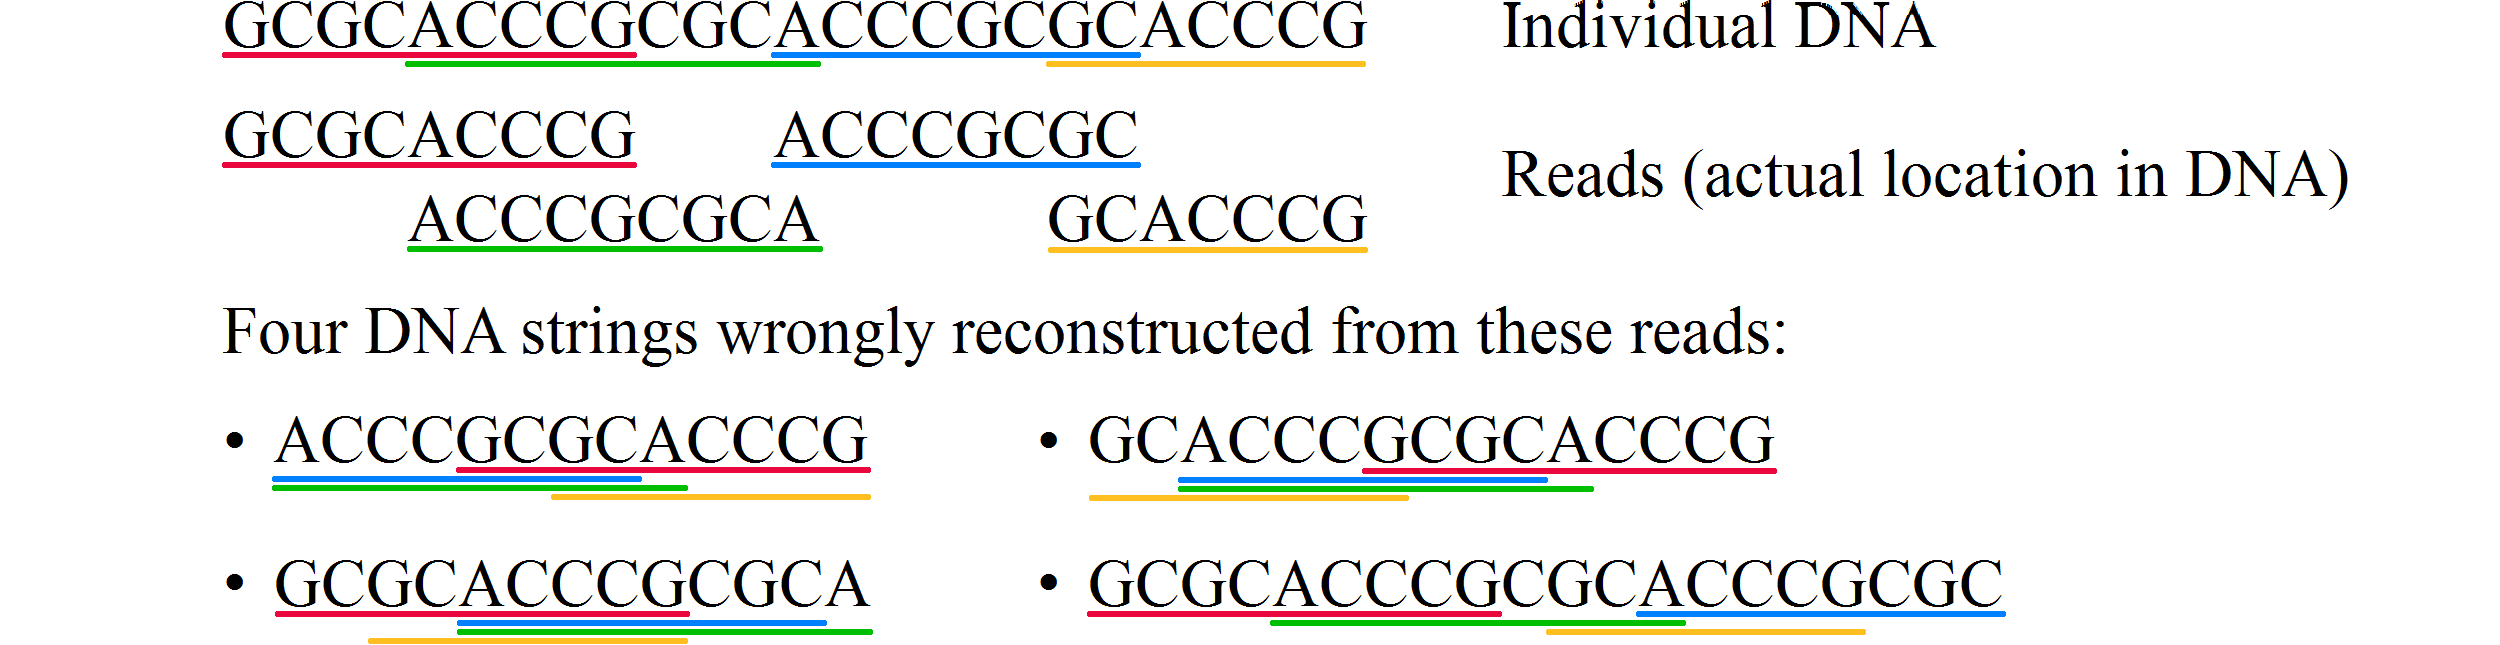
\includegraphics[width=\textwidth]{evo_intro_assembly_wo_reference.png}
\caption[Assembling an individual's DNA from small reads without a reference]{Problems with assembling an individual's DNA from small reads without a reference. Four possible reconstructions of the individual's DNA are shown, which all correspond to the observed reads, but are different from the actual DNA of the individual.} \label{fig:evo_intro_assembly_wo_reference}
\end{figure}
One purpose of the reference is therefore to guide the construction of the individual DNA in a meaningful way.
% TODO :: add picture and some text, saying: E.g. if we have the reads BLA then we could assemble them like BLA BLA,
% but with a reference we get BLAAABBEL...

Another purpose of using a genomic reference becomes clear 
in the case of diagnosing a disease in a patient. 
It is usually not very helpful to build the patient's full individual DNA, as the plain DNA string without 
annotations would not give us any information. 
% TODO :: citation needed
Instead, we are interested only in the variations from the norm, 
as these might be known to be associated with a specific disease. 
By aligning the reads to the reference, the software pipeline can keep track 
of the encountered differences and in the end give out a list of differences between the individual and the reference. 
An example for the process leading to such a list of differences 
can be seen in figure~\ref{fig:evo_intro_general_variation_calling_process}. 
\begin{figure}[!htb]
\centering
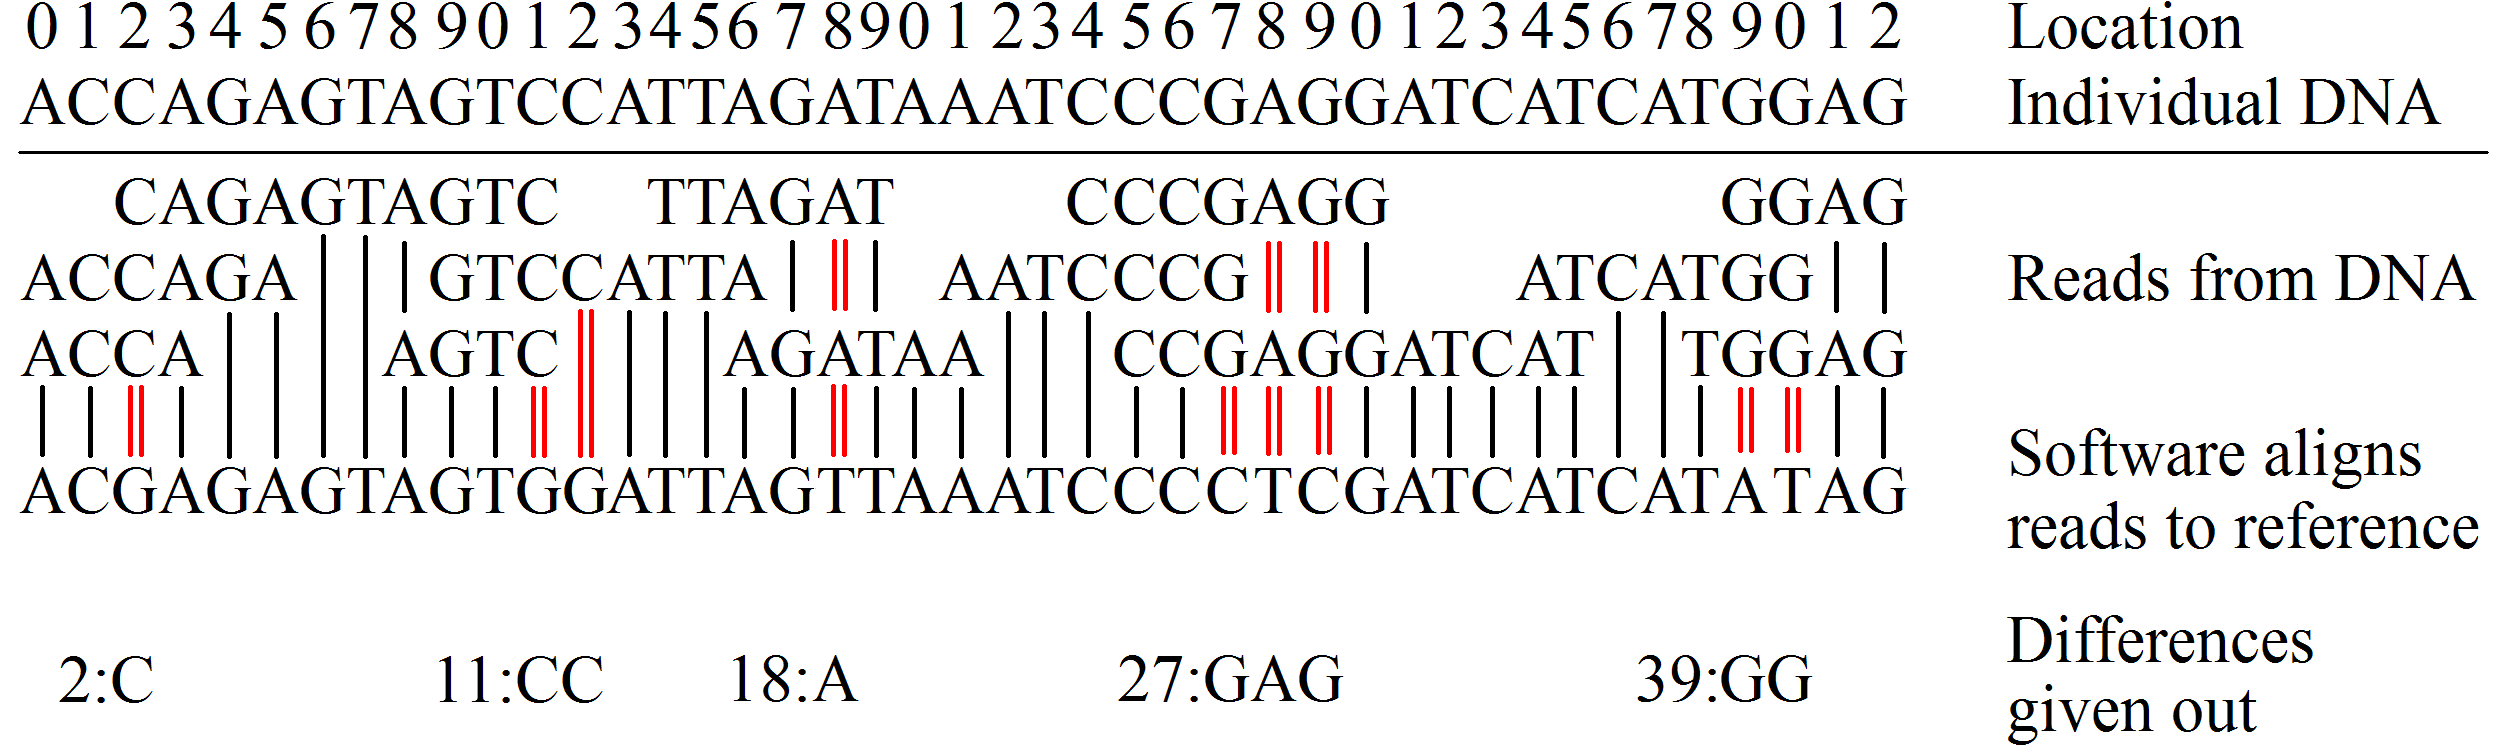
\includegraphics[width=\textwidth]{evo_intro_general_variation_calling_process.png}
\caption[General variation calling process]{General process for generating a list of variations between the individual DNA and the reference.} \label{fig:evo_intro_general_variation_calling_process}
\end{figure}
The alternative would be to construct the entire individual genome, and upon being done with this enormous task to 
compare the genome with a reference to find all the differences. This comparison however would be a sizeable 
and difficult alignment problem in its own right, so that it is more sensible to align the reads directly to the reference 
and give out the differences that were found in that way.

The reference therefore serves both as a blueprint while aligning the reads, 
as well as an anchor point to which variations within the individual string can be marked.

\section{The Reference Graph}

Traditionally, the reference is a compressed genomic string. 
In its simplest form it can be thought of as a plain text containing only the letters 
A, C, G and T. \\
It is rather straightforward to use such a reference string. 
Each location within the string can clearly be identified by its position---that is, 
its distance from the start. \\
Also, there are very simple file formats available to work with 
such references. One of these is the FASTA format, which includes the genomic 
strings together with lines for free text comments and with line breaks which 
make it easier to display the file in even low level text editors.
% TODO :: citation or link needed for FASTA (also, is it called FATA

The simplicity of reference strings however also has disadvantages. 
Most importantly, when aligning reads to a reference string, we can only align 
the reads to the average human genome, instead of aligning them to all known 
variations of the human genome at once. 
Not taking the known variations into account can lead to worse alignment results 
than would be possible otherwise, as the average genomic string may simply not 
include the particular mutations that have occurred for both the individual 
whose DNA is supposed to be read out as well as for another individual whose 
variations from the reference are known.

This is not just a theoretical consideration. 
Researchers now have access to annotated population variations, which augment the reference sequence string. 
These annotated variations can be found in databases of common variations, such as the publicly available  
dbSNP\footnote{\,\,\,\url{http://www.ncbi.nlm.nih.gov/SNP/}} 
and SNPedia\footnote{\,\,\,\url{http://www.snpedia.com/}}. 
Even the latest release of the Human Reference Genome, 
which is designated GRCh38
\footnote{\,\,\,\url{http://www.ncbi.nlm.nih.gov/projects/genome/assembly/grc/human/}}, 
contains alternative haplotypes for some complex regions, 
which are essentially known variations of the rigid reference string. \\
Considering that many alternative references are available and a lot of short variations are known, 
it becomes clear that the human genome should be thought of as a collection of individual genomes 
rather than a single rigid reference genome.

Algorithmically, this corresponds to viewing the reference as a graph rather than a linear genome. 
On this graph, each variation can be represented as a branch which points to the available alternatives. 
Thereby each personal genome is represented by a path through this variation graph, 
as can be seen in figure~\ref{fig:evo_intro_three_ref_seq_align}. \\
% TODO :: in the following picture, also add a graph interpretation underneath what I am seeing
%         (I want to see nodes and edges!)
\begin{figure}[!htb]
\centering
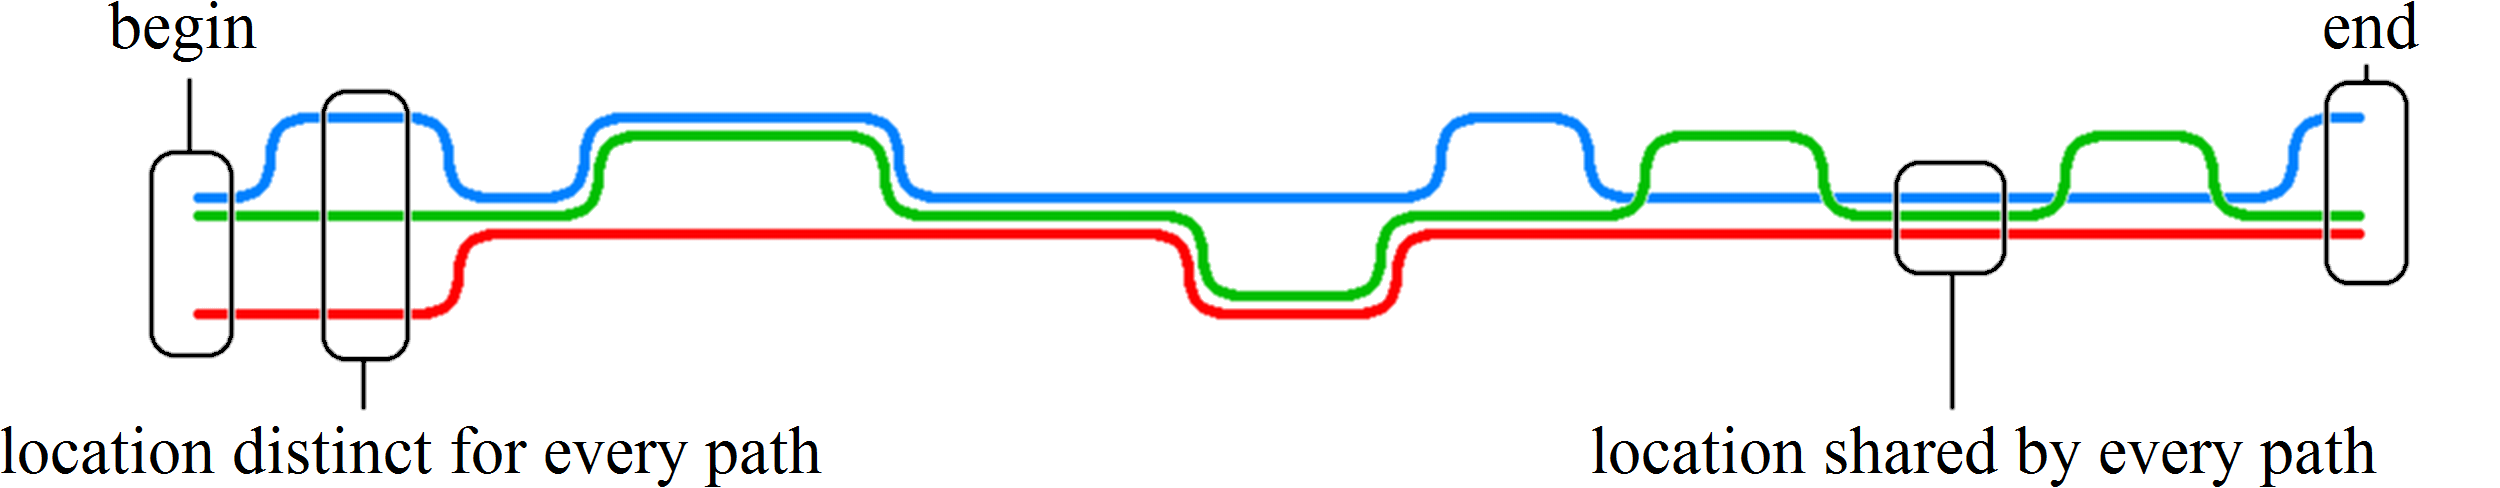
\includegraphics[width=\textwidth]{evo_intro_three_ref_seq_align.png}
\caption[Schematic visualization of three paths through a variation graph]{Schematic visualization of three paths through a variation graph, each representing an individual's genome.} \label{fig:evo_intro_three_ref_seq_align}
\end{figure}
This approach simplifies the identification of common variants, as a variant caller can 
ideally just note which path has been taken through the reference graph instead of having to 
explicitly state which differences have been found in which positions. \\
Using a reference graph also makes it possible to pick up combinations of variants 
which would currently be lost in the alignment step. 
Especially the calling of indels, which are usually harder to find and identify than edits, 
can benefit from having local access to several alternative references which contain 
already known variants \citep{Albers2010}.

Another advantage of using a reference graph presents itself when the continuous use of 
references over time is considered. 
When a new version of the human reference genome is published, 
it can take several years for research projects to adapt it, 
as existing pre-processed, aligned and annotated files all have to be updated \citep{RedditSwitchTo38}. \\
If instead a reference graph was underlying all alignments, it would be conceivable 
to update parts of that reference graph without changing the overall indexing of the entire structure, 
making it possible to seamlessly work with different versions of the entire structure. 
A possible way for a graph implementation to support this behaviour is by using a designated main 
reference that is unlikely to change often as the main indexing authority and by adding on top of it 
variations based on other references which can be changed out without changing the overall index.

Unfortunately, to fully implement a reference graph rather than a linear reference 
it is necessary to make drastic changes to all of the existing tools in the analysis pipeline. 
Such changes include the handling of new file formats which are capable of containing graph data, 
as well as changing the internal algorithmic logic of these tools to work on graphs.

\section{Thesis Motivation}

The focus of this thesis is therefore on the creation of an overview of the existing 
approaches that can be used for the implementation of genomic graphs, 
as well as on the exploration of new ways of working with genomic graphs, 
such as merging compressed graphs implicitly or explicitly. \\
The goal hereby is not mainly to create a new read alignment tool that uses 
a reference graph, but rather to create and implement new algorithms that can 
be used in conjunction with such graphs in the future.

Both the newly created algorithms as well as already established ones 
for the conversion of graphs between different internal formats 
will be implemented in such a way that their inner workings 
are directly observable. This simplifies the future usage of these algorithms 
within the scope of various parts of the analysis pipeline.

\chapter{Background}
% was ANDERE Menschen bisher so getan haben
%
% ====================================================================================================================================
%                                                                                                                           BACKGROUND
% ====================================================================================================================================

Nowadays there are many approaches for aligning short reads to a reference string, 
and even some work into the alignment of reads to a reference graph has already been 
undertaken. 
We will first focus on the BWT for strings, which is the basis for the more advanced 
XBW approaches for genomic graphs considered later on.

\section{Burrows--Wheeler Transform for Strings}

The core problem of read alignment to a reference string is simply that a 
lot of data needs to be worked on, as both the reference itself is very big 
and the amount of reads is enormous. \\
This actually leads to two distinct problems, the first being that the 
memory requirements for storing any of the required data are huge, 
and the second being that the time that is spend aligning reads for 
even just a single individual is very long.

To counteract the first problem, the data that is worked on is usually compressed, 
which means mostly that the string reference is being compressed in a certain way. 
Compressing the reads is not as helpful as compressing the reference, 
due to the fact that we can re-use the same compressed reference for aligning the 
reads of another individual later on, without having to execute the lengthy 
process of compressing the reference twice, while the reads will be different 
each time and therefore compressing them would mean that they have to be compressed again the next time around. \\
A method that has been applied very often to enable such a compression is the utilization of the 
Burrows--Wheeler Transform \citep{Burrows1994}, which 
is a reversible reordering of a 
repetitive text with few runs into a text of the same length that contains more runs 
and can therefore be easily compressed by run-length encoding or other encoding schemes. 
A simple example of this behaviour of achieving more easily compressable strings through the application of the BWT 
can be seen in table~\ref{table:evo_background_bwt_run_enc}. 
\begin{table}[htb]
\centering
\caption[Run-length encoding comparison between a repetitive string and its BWT]{Run-length encoding comparison between a highly repetitive string and its BWT. In this example, the run-length encoding of the string itself does not reduce the size, while the run-length encoding of the BWT reduces the size by 29\%.}
   \begin{tabularx}{\textwidth}{ | X | X | }
   \hline
   AGCAGCAGCCTTCTTAGCCTT & \textbf{Original string} \\
   AGCAGCAG\,2C\,2TC\,2\,TAG\,2C\,2T & \textbf{Original string run-length encoded} \\
   \hline
   TCTCGGGGCTCAAAATTTCCC & \textbf{BWT} \\
   TCTC\,4\,GCTC\,4A\,3\,T\,3C & \textbf{BWT run-length encoded} \\
   \hline
   \end{tabularx}
\label{table:evo_background_bwt_run_enc}
\end{table}
As the transformed text contains all the information necessary to recreate the 
original text, it is not necessary to store the original text at all.

A simple algorithm to generate the BWT of a string uses 
the concept of \textit{cyclic rotations}. 
The $ n $th cyclic rotation of a string is a reordering of the string in which its first $ n $ characters 
are taken away from the beginning of the string and are instead inserted at its end. \\
To generate the BWT of a string $ s = c_1 c_2 ... c_k $ of characters $ c_i $, 
we can generate all the cyclic rotations from $ n = 0 $ up to $ n = k - 1 $, and 
put the resulting strings on a list. 
We then sort this list alphabetically, and write out the resulting list of strings 
in such a fashion as to have each of the strings on its own row, exactly underneath each other. 
This creates a matrix of characters, of which we take the last column. 
Read from the top to the bottom, this last column is the BWT of string $ s $. 
This algorithm is also illustrated in figure~\ref{fig:evo_fig_bwt_with_cyclic_rotations}.

\begin{figure}[!htb]
\centering
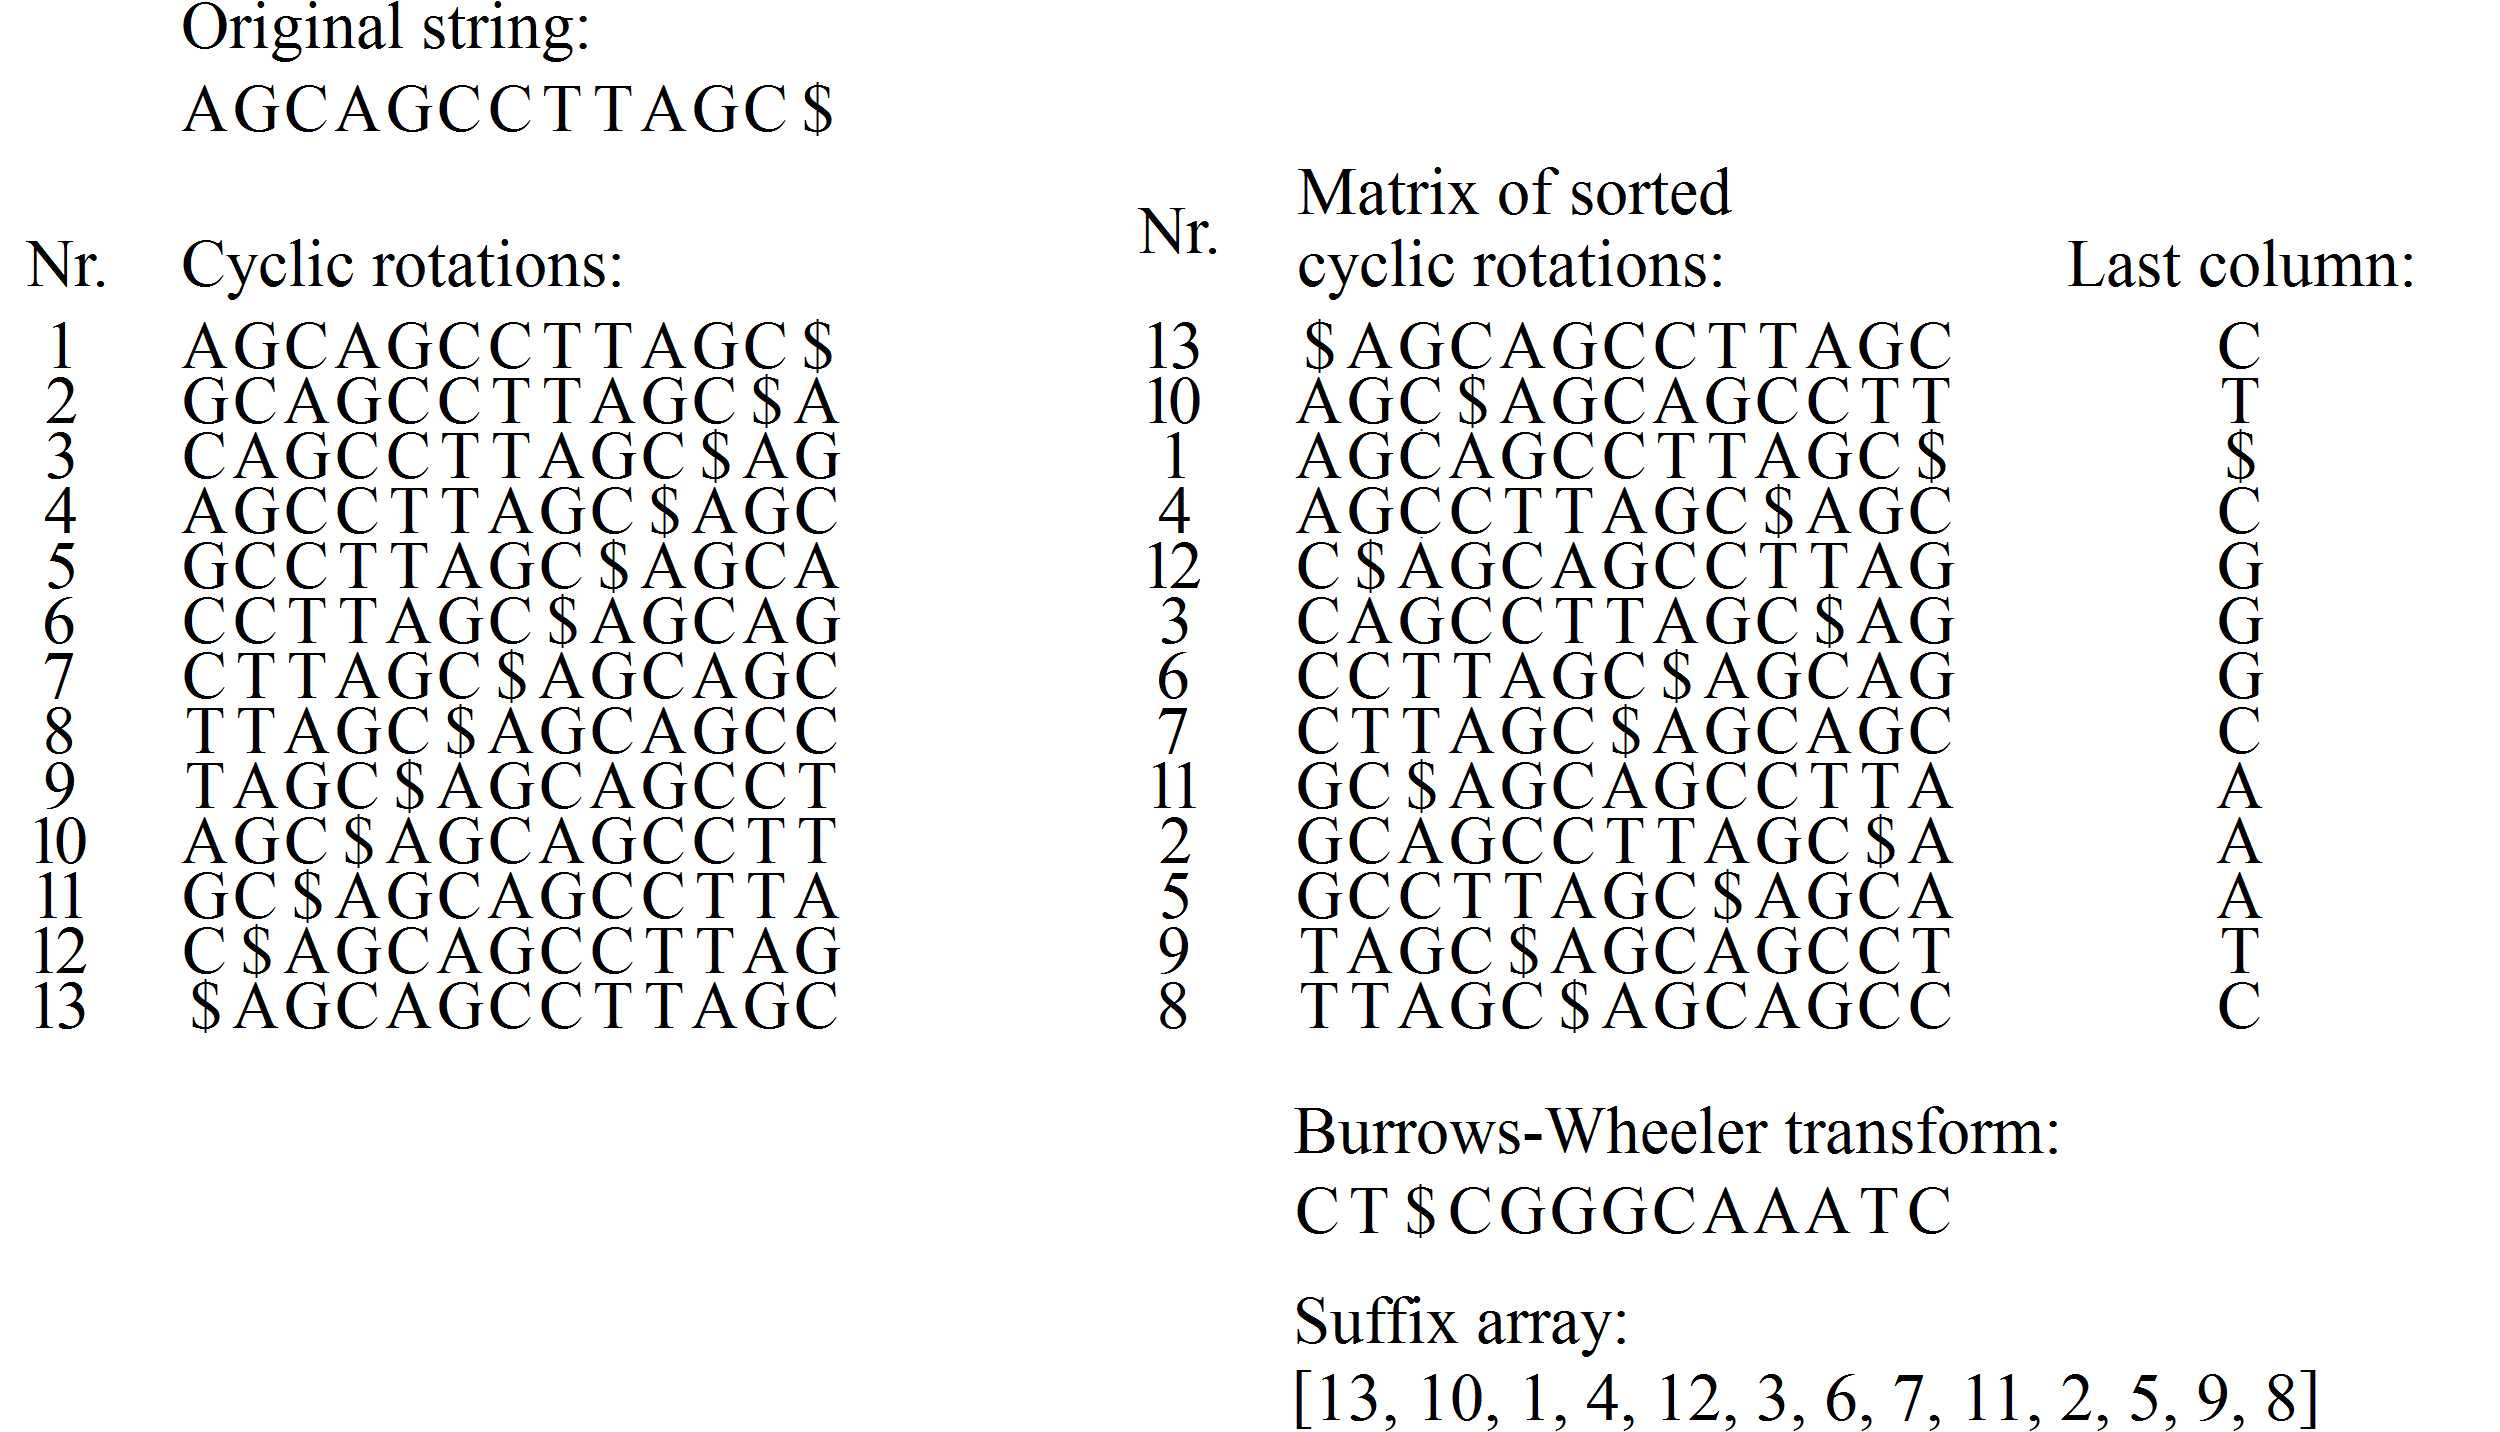
\includegraphics[width=\textwidth]{evo_fig_bwt_with_cyclic_rotations.png}
\caption[Generating the BWT of a string]{Generating the BWT of the string $ s = \textup{AGCAGCCTTAGC\$} $. After generating a list of cyclic rotations, the list is sorted, and the last column of the matrix formed by this sorted list reveals the BWT of $ s $ to be \textup{CT\$CGGGCAAATC}.} \label{fig:evo_fig_bwt_with_cyclic_rotations}
\end{figure}

It is customary to append a certain character to the end of the string before generating its BWT, 
with that character being different from all other characters in the string. 
A usual choice for this character is the dollar sign “\$”. \\
The reason for appending such a character is the requirement of being able to reconstruct the original string 
from the BWT, which allows us to discard the original string after encoding it using the BWT 
and compressing it with run-length encoding. 
Without a dedicated character telling us where the end of the string is located, 
the matrix of alphabetically sorted cyclic rotations could be reconstructed from the BWT, 
but it would be impossible to decide which one of the rows in that matrix represented the original 
string, as cyclic rotations based on each row would alphabetically sorted to the exact same matrix. 
Instead of adding a distinctly different character to the end of the string, 
it is therefore also possible, although not customary, to simply store an integer with the BWT containing 
the number of the row within the matrix which contains the original string \citep{Nelson1996}.

As mentioned before, it is crucial that the BWT is a reversible reordering of a string, 
such that the original string can be obtained from the BWT. 
A simple algorithm for recreating the original string given its BWT starts by reconstructing the alphabetically sorted 
matrix of cyclic rotations as empty $ n {\times} n $ matrix, where $ n $ is the length of the BWT. 
The last column of the matrix is then filled with the BWT, spelled out vertically. 
All the rows in the matrix are then sorted alphabetically. 
Now, the second-to-last column of the matrix is filled with the BWT, 
and again all the rows in the matrix are sorted alphabetically. \\
This inserting of the BWT in the right-most empty column and subsequent alphabetical sorting of all rows 
is continued until the matrix has been filled entirely. 
The original string now consists of the first $ n - 1 $ characters in the row in the matrix which 
ends with the special character, 
usually the dollar sign.

% TODO :: add figure to the BWT reverting?

As noted before, the given algorithm for the creation of the BWT is rather simple, 
and more efficient algorithms exist which do not require building up the entire matrix of cyclic rotations. 
Likewise, the algorithm for regaining the original string from the BWT is not customarily 
used in its form here in practice. \\
Actually, many current alignment tools such as BWA-MEM \citep{Li2013} and Bowtie \citep{Langmead2009} which use 
the BWT to compress the reference actually 
work on the reference in this compressed form directly, without having 
to recreate the original text in its entirety in memory.

As memory has gotten cheaper over time and machines have become more 
well-equipped, memory consumption nowadays is not as much of a concern 
as it once was, when just fitting the reference into memory 
took a lot of ingenuity. \\
% TODO :: citation needed
However, the memory utilization of alignment tools is still important, 
as further reductions in the overall amount of memory necessary would 
mean that the alignment could be done using smaller and therefore cheaper 
machines, which would open up more real-world applications for sequence analysis 
for which its price currently is still too high.
Also, a focus on how the available memory is used could lead to new alignment 
tools that make more efficient use of the special memory that is more readily available 
for the processor, such as using the L1, L2 and L3 cache rather than sending a lot of 
requests to the slower general RAM. \\
Therefore, research into methods reducing the memory requirements of alignment tools 
is still ongoing.
% TODO :: citation needed? maybe?

\section{The Role of Graphs in Read Alignment}

Initial use of graphs in read alignment was restricted to representing 
the outcome of the alignment phase, in particular the fully assembled DNA \citep{Myers2005}.

Short reads usually do not make it possible to fully infer the actual structure of the genome that is read out, 
as different possible structures could have lead to the same reads, especially when considering that 
there are many errors within the reads that need to be accounted for. \\
Therefore, often the reads are aligned to a reference and the best fitting position is simply 
assumed to be the real origin of the read. However, as the decision to choose one position over 
another can be quite arbitrary, graphs can be used as read alignment output which indicate how the reads 
are linked together. The true individual DNA that was read out is then one possible path through the graph, 
while other possible paths through the graph exist that are merely artefacts of the sequencing process. \\
As such a graph can be quite difficult to work with, not many alignment tools are producing these 
structures. Instead, the default is usually to just choose the best fitting position and 
create a read out DNA string. This string will most likely also contain some sequencing artefacts, 
but will be vastly easier to work with in later steps.

Graphs are currently also starting to be used as a way to reduce the size of several read out human 
genomes \citep{Li2014}. \\
The idea stems from the fact that companies or institutions that read out the DNA of several individuals 
and want to store them can run in problems with the immense file size when storing or transmitting the reads and their 
aligned locations. Instead, the original read data could be discarded and only the alignment result could be saved and shared---that 
however would mean that the original data cannot later on be re-interpreted by better algorithms, and can in general 
not be used any more. \\
Using a graph in this case can allow several agreeing reads to be combined into long sequences of unambiguous data, 
while the locations at which uncertainties exist could still be encoded with all the possible alternatives as 
different paths through the graph. Therefore, all complicated read data behaviour is contained in the resulting 
graph, but the size is still vastly reduced when compared to using all reference strings of the population.

\section{Formal Graph Definition}
\label{sec:graph_definition}
%
% ~~~~~~~~~~~~~~~~~~~~~~~~~~~~~~~~~~~~~~~~~~~~~~~~~~~~~~~~~~~~~~~~~~~~~~~~~~~~~~~~~~~~~~~~~~~~~~~~~~~~~~~~~~~~~~~~~~~~~~~~~~~~~~~~~~~~
%                                                                                                  BACKGROUND: Formal Graph Definition
% ~~~~~~~~~~~~~~~~~~~~~~~~~~~~~~~~~~~~~~~~~~~~~~~~~~~~~~~~~~~~~~~~~~~~~~~~~~~~~~~~~~~~~~~~~~~~~~~~~~~~~~~~~~~~~~~~~~~~~~~~~~~~~~~~~~~~
We define a \textit{graph} $ G = (V, E) $ as a collection of a set 
of \textit{nodes} $ V = \{ v_1, ..., v_{|V|} \} $ and a set of edges $ E {\: \subseteq \:} V^2 $. 
Each one of these edges is a set $ (u, v) {\: \in \:} E $ with $ u {\: \in \:} V $ and $ v {\: \in \:} V $, 
which we call an edge from node $ u $ to node $ v $. 
As the graphs we are working with are considered to be \textit{directed}, 
we assume edge $ (u, v) {\: \in \:} E $ to 
be distinct from edge $ (v, u) {\: \in \:} E $. 
An example of such a graph can be seen in figure~\ref{fig:evo_fig_graph_example}. \\
% GACGT|,2,T,4;,3,,5 vs. ACCTG|,1,,5;,1,,3 without start and end nodes
\begin{figure}[!htb]
\centering
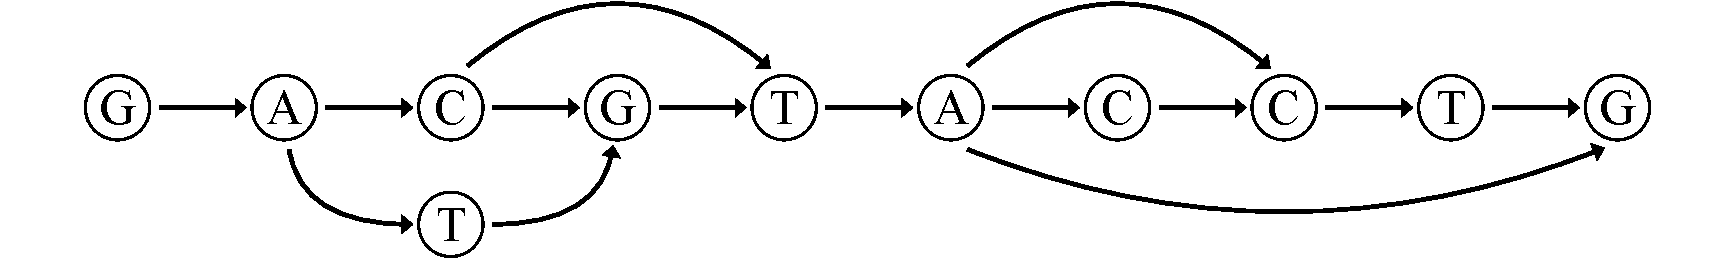
\includegraphics[width=\textwidth]{evo_fig_graph_example.pdf}
\caption[Example graph]{Example graph with 11 nodes and 14 edges.} \label{fig:evo_fig_graph_example}
\end{figure}
For every node $ v {\: \in \:} V $ we define the amount of incoming edges of 
node $ v $, or the \textit{indegree} $ \textrm{in} ( v ) $, as the number of 
distinct edges $ (u, v) {\: \in \:} E $ for any $ u {\: \in \:} V $. 
Similarly, for every node $ v {\: \in \:} V $ we also define the amount of outgoing edges of 
node $ v $, or the \textit{outdegree} $ \textrm{out} ( v ) $, as the number of 
distinct edges $ (v, u) {\: \in \:} E $ for any $ u {\: \in \:} V $. \\
The graphs considered here are \textit{labelled}, which means that a label $ l( v ) $ is attached 
to every node $ v {\: \in \:} V $. 
Every label $ l( v ) $ represents a character 
from the alphabet $ \Sigma $, which is a set of characters. 
In principle, a label could also consist of several characters, 
but we limit each label to exactly one character as we wish to 
represent several characters as nodes with separate labels sequentially connected by edges. 
We refer to such a structure of sequentially connected 
nodes $ u_1, u_2, ..., u_n $ as \textit{path} $ P = u_1 u_2 ... u_n $.

\section{Burrows--Wheeler Transform for Graphs}

Graphs have not only been used to indicate the results of the read alignment. 
The alignment of short reads to a reference graph rather than to a linear reference has 
also been proposed several times.

A necessary prerequisite for aligning reads to a reference graph is 
being able to actually create such a graph in the first place. \\
One of these ways is to take several similar genomic strings and create a graph based 
on them, such that each of the input strings is a path through the resulting graph. 
\citet{Lee2002} proposed a method to create such a graph from input strings, 
independent of the order in which these strings 
are added to the emerging graph.

Storing several very similar references at the same time in a way that not only minimizes 
the storage space, but also enables efficient pattern searches directly on the 
stored data was proposed by \citet{Makinen2010}. \\
The aim of these techniques is to 
minimize both the overhead in storage space and the needed time to perform typical work 
on the references, such as aligning reads to them.

This group of authors continued working with scenarios in which 
several references are merged into a graph, with reads being directly 
aligned to the graph rather than to each reference on its own \citep{Siren2014}. \\
The alignment of reads against the data structure incorporating several references 
is done in a way that is inspired by the Burrows--Wheeler Transform. \\

In particular, to be able to use the Burrows--Wheeler Transform for read alignment, 
a data structure called the suffix array \citep{Puglisi2007} is commonly used, which contains 
information about the locations within the reference. 
Using the suffix array makes it easier to work on the BWT in its compressed form, 
rather than having to reconstruct the original string from it to perform work. 
That is, the BWT together with its suffix array forms a self-index, 
which is a data structure that contains compressed data and makes it possible 
to work on that data directly in its compressed form \citep{Navarro2007}. \\
As indexing a graph based on several references is not as straightforward as 
indexing a single string, which provides an inherent indexing mechanism by 
simply stating the position within the string, the regular suffix array cannot 
be used in the case of encoding a graph rather than a string. \\
However, the plain suffix array is often not used in a practical sense 
without any changes anyway. Instead, it is often compressed in some way or another. 
The reason for that is the immense size of the regular suffix array. 
A common compression technique is to leave out many of the suffix array's parts 
and instead compute them dynamically 
when they are being used rather than storing the entire array in memory. 

When using a reference graph for read alignment with the BWT, it is therefore common 
already to use a structure that simply behaves similar to the suffix array. 
Such a suffix-array-like data structure can also be constructed for graph references.

In particular, efficient support of the following operations is necessary for such a data structure \citep{Siren2014}: \\
Given a pattern, the range within the data structure 
that corresponds to all suffixes of the reference graph that are prefixed with that pattern needs to be found. 
This essentially provides a functionality for finding arbitrary texts, and is used when aligning reads to 
the reference, as that is basically a search for the read itself or similar patterns within the reference. \\
Given a location within the data structure, the corresponding location within the 
reference needs to be located. \\
Finally, given a location within the reference, the actual text at that position 
needs to be extracted.

The main idea is therefore to create a structure capable of fulfilling these requirements, 
as the remainder of the alignment step is then very similar to the alignment against a reference string.

\section{Alignment Without an Actual Graph}

To avoid the complications arising when working with 
a complete graph made from several references, other methods have been proposed 
to achieve similar results without explicitly constructing a reference graph.

One of these is the alignment tool BWBBLE which 
was created by \citet{Huang2013}. \\
It works on the core assumption that most differences in between two references 
are snips, which can be encoded with a specific extended alphabet. 
Then, a modification to the Burrows--Wheeler Transform is made to 
be able to work with a single string reference containing this extended alphabet. \\
BWBBLE also supports insertions and deletions which means that it does support 
more graph-like behaviour, but the core functionality of it is aimed at the extended string reference.

In addition, there have been efforts to more efficiently create the BWT 
of several strings rather than just concatenating them into a single one. 
These can help in understanding the challenges of building the BWT of several references \citep{Holt2014}.

\section{Using Hashes to Encode a Graph}

The hashing approach focuses also on a certain way of pre-processing the references 
to create a certain structure that the reads can then be aligned against. \\
To use this approach, a specific length $ k $ is given, up to which we keep track of 
sequences in the reference graph.

In the pre-processing step, among all the possible references one main reference is chosen. 
Then a hash table based on the references is created which 
assigns each $ k $-mer the positions at which it can be found. 
Such a position is not as straightforward as a 
plain integer that gives the index within a string, as the data can lie on branches 
off the main reference string. \\
This is solved by using an integer together with minor extra information. 
The integer points towards a data block, which can be a part of the main 
reference or a branch of any of the other references that differs from the 
main sequence. The extra information then points towards the location within the block.

In particular, aligning reads to several references at once 
in this way has been proposed by \citet{Schneeberger2009}. \\
In this case, the references are taken together to form a graph 
rather than being used as separate reference strings. 
For this to be achieved, all references are pre-processed in a special way, with one being taken as the 
main reference and the other references being stored as changes to this main reference. 
The pre-processing step results in a data structure that uses $ k $-mers as hashes pointing 
to the specific location at which these $ k $-mers can be found. Reads can therefore be aligned 
by finding parts of them in the hash table, looking up the locations that are associated with 
them, and checking if the entire read can be aligned to that location. \\
The location here is not just an integer pointing to a character within a string, 
as it would be for a single reference, but actually 
a pointer to the particular reference and the location within it. 
To make this indexing possible, the references are split into blocks that 
can quickly be addressed with an integer and locations within those blocks.

When the reads are aligned against the data structure, the output of the alignment step 
can be generated in two ways---either with each read being aligned to the particular reference 
that it agrees with most, or with each read being aligned in the same way but with the 
alignment afterwards being rewritten as if the read was aligned to the main reference. \\
This second option makes it possible to use this approach even as part of an already existing pipeline 
built for a reference string, not a reference graph, if losing some of the benefits of 
the graph alignment is acceptable. However, to fully utilize all the graph information, 
the rest of the pipeline has to be adapted as well.

\section{Extending the Burrows---Wheeler Transform}

Efforts involving changes to and generalizations of the Burrows--Wheeler Transform 
are also aided by the development of the XBW, which is a 
method of compressing trees similar to how the BWT is used to compress sequential data \citep{Ferragina2009}. \\
Each node in the tree has a label that is one character long. 
These labels are stored in the XBW together with a special bit vector, 
which keeps track of whether a given node is a leaf node or not. 
That is, if a node has a successor, then this bit vector takes the value 0, as that node is not the last node 
of its branch. If a node does not have a successor, then the bit vector takes the value 1 for that node. \\

\citet{Siren2014} extended the XBW even further, by introducing a second bit vector that enables nodes 
to have multiple predecessors as well as multiple successors. Therefore, this extended XBW can not only 
store trees, but instead can keep track of general finite graphs. 
In this paper, the extended XBW is stored in two different kinds of data structures, 
which have not been given explicit names there. We refer to these structures as 
node tables and flat tables.

\subsection{Node Tables}
\label{sec:node_table_definition}

We decided to refer to the first of the two data structure as XBW node table, or just node table, 
as it is a 
table containing the extended XBW which contains exactly one column for each 
node of the graph represented by the extended XBW. \\
More formally, we define:

\textbf{Definition} An \textit{XBW node table}\label{def:node_table} is a table with rows for the BWT, 
the prefixes and the values of the bit vector $ M $, 
representing a finite graph with each column of the table corresponding 
to exactly one node of the graph.

The columns in a node table are sorted alphabetically by the given prefix. 
For any column $ i $ representing node $ v_i $ in the graph, 
the value of the BWT in column $ i $ represents the labels of the nodes 
preceding $ v_i $. 
If several nodes with different labels are preceding the node $ v_i $, 
then the BWT value takes on the concatenation of all these values. 
To make it clearer that a BWT containing several characters actually 
stands for any of these characters, instead of standing for the string 
formed by the characters, we decided to display BWT values containing 
more than one character separated by pipe characters, as can be 
seen in figure~\ref{fig:evo_fig_node_table_example} which is represented 
by node table~\ref{table:evo_node_table_example}. \\
% GCTGGCGAG|,2,TT,5;,2,TGG,7
{
% reduce whitespace in this table (default might be 6pt)
\renewcommand{\tabcolsep}{2pt}
\begin{table}[htb]
\centering
\caption[Node table corresponding to a graph]{Node table corresponding to the graph in figure~\ref{fig:evo_fig_node_table_example}.}
\begin{tabular}{ | c | c | c | c | c | c | c | c | c | c | c | c | c | c | c | c | c | }
\hline
G & G & G & G & A & C|G & G|T & $\#$ & G & T & T & T & C & C & C & \$ & \textbf{BWT} \\ \hline 
\$ & A & CG & CT & G\$ & GA & GCG & GCT & GGA & GGC & GGG & TGC & TGGC & TGGG & TT & $\#$ & \textbf{Prefix} \\ \hline 
1 & 1 & 1 & 100 & 1 & 1 & 1 & 1 & 1 & 1 & 1 & 1 & 1 & 1 & 1 & 1 & $\boldsymbol{M}$ \\ \hline 
1 & 1 & 1 & 1 & 1 & 10 & 10 & 1 & 1 & 1 & 1 & 1 & 1 & 1 & 1 & 1 & $\boldsymbol{F}$ \\ \hline 
\end{tabular}
\label{table:evo_node_table_example}
\end{table}
}
% GCTGGCGAG|,2,TT,5;,2,TGG,7, just like above
\begin{figure}[!htb]
\centering
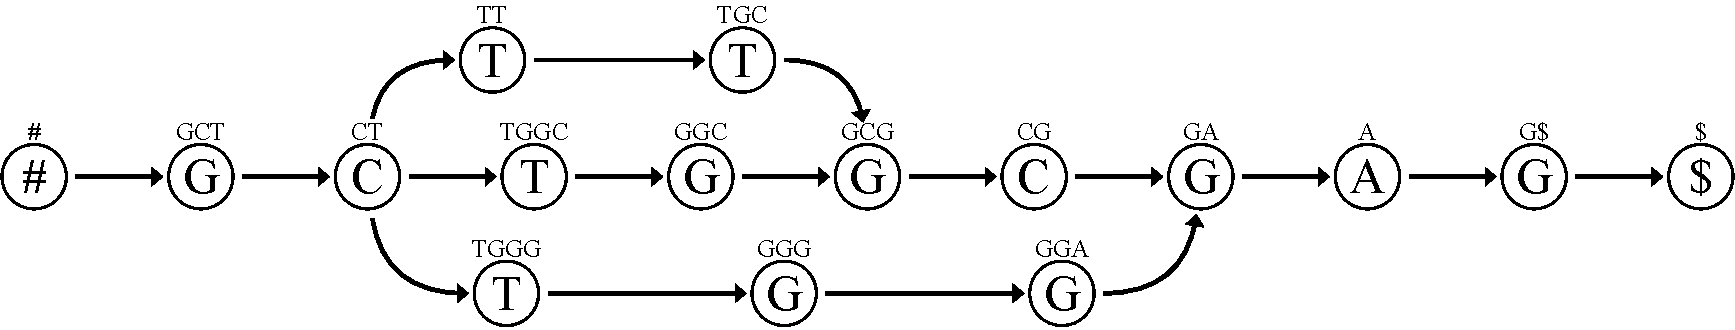
\includegraphics[width=\textwidth]{evo_fig_node_table_example.pdf}
\caption[Graph corresponding to a node table]{Graph corresponding to node table~\ref{table:evo_node_table_example}. The prefixes of the nodes have been provided in small print above the nodes, to make it easier to identify which node in the graph corresponds to which column in the table.} \label{fig:evo_fig_node_table_example}
\end{figure}
% TODO :: make sure that these two (the table and the figure) actually end up on the same page, and are not split over several pages
The value of the prefix in column $ i $ is precisely the prefix of node $ v_i $ in the graph, 
which is a string starting with the label of $ v_i $ and then containing 
the labels of the following nodes in sequence of encountering them traversing 
the graph outwards from $ v_i $.
The value of the cell $ M $ in column $ i $ is a sequence of bits whose length corresponds to 
the amount of successor nodes of $ v_i $, or equally the amount of outgoing edges of node $ v_i $. 
This sequence always starts with the bit “1” and is then followed 
by as many “0” bits as are necessary to achieve the desired length. 
In addition to bit vector $ M $, a second bit vector designed as $ F $ can be used within a node table. 
The value of $ F $ in column $ i $ is a bit sequence whose length corresponds to 
the amount of predecessor nodes of node $ v_i $. 
The reason why using the $ F $ bit vector is not strictly necessary is that its information 
for any column $ i $ is already encoded in the length of the BWT cell of column $ i $. 
When implementing $ M $ and $ F $, it is possible to think of them as arrays of strings, 
with each string containing the characters “1” and “0”, for ease of implementation.

\subsection{Flat Tables}
\label{sec:flat_table_definition}

In contrast to the previously introduced node table, 
we refer to the next data structure as flat XBW table, or just flat table. 
This name is inspired by the fact that the data of each row here is not 
stored as array with elements of various lengths, 
but instead as flat sequence of characters which can be encoded as string 
or as array with elements of fixed size. \\
The definition shows that a flat table consists of similar parts as a node table:

\textbf{Definition} A \textit{flat XBW table}\label{def:flat_table} is a table with rows for the BWT, 
the node labels and the values of $ M $ and $ F $, 
representing a finite graph. 
The table is arranged such that each cell contains exactly one character 
for the BWT and the node labels, and such that each cell contains exactly 
one bit for the bit vectors $ M $ and $ F $.

We here often refer to the row containing the node labels as first column row, or short “FC”. 
The reasoning behind this name is that the row of node labels of the graph relate to the BWT row, 
as the first column in the matrix of sorted cyclic rotations does to the last row, which is the traditional BWT. 
That is, the node labels are also the alphabetically sorted BWT, and in fact the columns are sorted in such a 
way that when the prefixes are generated for each column in turn, they are sorted alphabetically as well. \\
As the FC row simply corresponds to the BWT sorted alphabetically, it can easily be calculated 
when the BWT row is known. The BWT however, while being potentially very 
long, only consists of characters from a limited alphabet $ \Sigma $. 
Therefore, storing the FC both in a file and in memory does not take up a lot of storage space. 
This means that we usually accept the small space taken up by keeping it stored in memory, 
instead of recalculating it based on the BWT again and again. 
We can achieve this storage of FC using the array $ C $, which is another structure that can be generated 
from the BWT. \\
In fact, we usually calculate several structures from the BWT, $ M $ and $ F $ which 
can be used in conjunction with the flat XBW table. 
The additionally calculated information includes 
the alphabet $ \Sigma $, a set of all distinct characters encountered in the BWT. \\
We also keep track of the array “ord”, which has the characters of the alphabet as keys as their 
positions in the alphabetically sorted $ \Sigma $ as indices. \\
We finally generate the array $ C $, which also has the characters of the alphabet as keys, 
and whose values are the indices of the first occurrences of these characters within FC. 
The array $ C $ completely encodes FC, so that we do not need to explicitly store FC in any other way. 
Of course, we can do so anyway for a particularly simple implementation.

The bit vectors $ M $ and $ F $ are exactly the same as the corresponding bit vectors in the node table, 
and are each strongly related to one of the other rows. 
In particular, each cell in the $ M $ vector corresponds to a cell, or character, in the FC row, 
as each outgoing edge $ (u, v_i) $ of a node $ u $ corresponds to another cell in the $ M $ vector, and each 
of these outgoing edges shares the same node $ u $ in which it originates, therefore sharing the same label $ l ( u ) $, 
which is precisely the content of the FC row. \\
On the other hand, each cell in the $ F $ vector corresponds to a cell, or character, in the BWT. 
The reason for this is that the graph we are working on is necessarily reverse deterministic 
for this encoding to function properly, which is explored in further depth in section~\ref{sec:why_rev_det}. 
Due to that, the label $ l (u_i) $ for each incoming edge $ (u_i, v) $ into a node $ v $ is distinct, 
as the graph would otherwise not be reverse deterministic. 
Therefore, for every node $ v $ there are as many entries in the BWT, which contains the labels of the preceding nodes, 
as there are entries in the $ F $ bit vector, which keeps track of the amount of incoming edges.

Encoding the same graphs both as flat XBW tables and as node tables 
shows that flat XBW tables are much smaller and therefore easier to store. 
The biggest differences between the two kinds of tables, 
which can both be used to encode genomic graphs, 
are that flat tables do not contain the potentially enormously big prefix cells 
of node tables, and that flat tables do not require any overhead to 
keep track of column boundaries within a row. 
While node tables can contain strings of various sizes in all their cells, 
flat tables contain exactly one character in each cell, such that 
an entire table row can be stored as string without losing information 
about the cell boundaries. \\
This smaller size comes at the cost of simplicity. 
Within a node table, each column clearly corresponds to a node within the graph, 
and a simple manual inspection of the table can lead to various insights into the graph. 
In a flat table however, not every column describes and entire node within the graph, 
as some columns only describe parts of nodes, as e.g. a node with several predecessors 
can have information about its BWT spread across several columns in the flat table. 
We therefore should not even think about whole columns in the flat table, 
but instead of clusters of cells which correspond to nodes. 
We use the $ M $ and $ F $ rows to 
find these cell clusters across different rows, which for graphs with high in- and outdegrees 
are not necessarily located in columns that are even close together.
How cells in a flat table relate to actual nodes in a graph is illustrated via specifically highlighted 
cells in table~\ref{table:flat_table_with_ct}, which corresponds to the graph with highlighted nodes 
in figure~\ref{fig:evo_fig_flat_table_with_ct}. \\
{
% reduce whitespace in this table (default might be 6pt)
% \renewcommand{\tabcolsep}{5pt}
% GCTGGCGAG|,2,TT,5;,2,TGG,7, searching for CTTG
\begin{table}[htb]
\centering
\caption[Flat table corresponding to a graph]{A flat XBW table with cells highlighted that correspond to four nodes in the graph in figure~\ref{fig:evo_fig_flat_table_with_ct} represented by this table. The alphabet for this table, including the labels of the start and end node, is $ \Sigma = \{ \textup{\$, A, C, G, T, $\#$} \} $. The \textup{ord} array is $ [ \$ {\, \Rightarrow \,} 0, \textup{A} {\, \Rightarrow \,} 1, \textup{C} {\, \Rightarrow \,} 2, \textup{G} {\, \Rightarrow \,} 3, \textup{T} {\, \Rightarrow \,} 4, \textup{$\#$} {\, \Rightarrow \,} 5 ] $ and the $ C $ array is $ [ \$ {\, \Rightarrow \,} 0, \textup{A} {\, \Rightarrow \,} 1, \textup{C} {\, \Rightarrow \,} 2, \textup{G} {\, \Rightarrow \,} 6, \textup{T} {\, \Rightarrow \,} 13, \textup{$\#$} {\, \Rightarrow \,} 17 ] $.}
\begin{tabular}{ | c | c | c | c | c | c | c | c | c | c | c | c | c | c | c | c | c | c | c | }
\hline
G & G & G &\cellcolor{purple_bg}\color{purple_fx}G & A & C & G &\cellcolor{green_bg}\color{green_fx}G &\cellcolor{green_bg}\color{green_fx}T & $\#$ & G & T & T &\cellcolor{red_bg}\color{red_fx}T & C & C &\cellcolor{blue_bg}\color{blue_fx}C & \$ & \textbf{BWT} \\ \hline 
\$ & A & C &\cellcolor{purple_bg}\color{purple_fx}C &\cellcolor{purple_bg}\color{purple_fx}C &\cellcolor{purple_bg}\color{purple_fx}C & G & G &\cellcolor{green_bg}\color{green_fx}G & G & G & G & G &\cellcolor{red_bg}\color{red_fx}T & T & T &\cellcolor{blue_bg}\color{blue_fx}T & $\#$ & \textbf{FC} \\ \hline 
1 & 1 & 1 &\cellcolor{purple_bg}\color{purple_fx}1 &\cellcolor{purple_bg}\color{purple_fx}0 &\cellcolor{purple_bg}\color{purple_fx}0 & 1 & 1 &\cellcolor{green_bg}\color{green_fx}1 & 1 & 1 & 1 & 1 &\cellcolor{red_bg}\color{red_fx}1 & 1 & 1 &\cellcolor{blue_bg}\color{blue_fx}1 & 1 & $\boldsymbol{M}$ \\ \hline 
1 & 1 & 1 &\cellcolor{purple_bg}\color{purple_fx}1 & 1 & 1 & 0 &\cellcolor{green_bg}\color{green_fx}1 &\cellcolor{green_bg}\color{green_fx}0 & 1 & 1 & 1 & 1 &\cellcolor{red_bg}\color{red_fx}1 & 1 & 1 &\cellcolor{blue_bg}\color{blue_fx}1 & 1 & $\boldsymbol{F}$ \\ \hline 
\end{tabular}
\label{table:flat_table_with_ct}
\end{table}
}
% GCTGGCGAG|,2,TT,5;,2,TGG,7, searching for CTTG, with colors inverted, just like above
\begin{figure}[!htb]
\centering
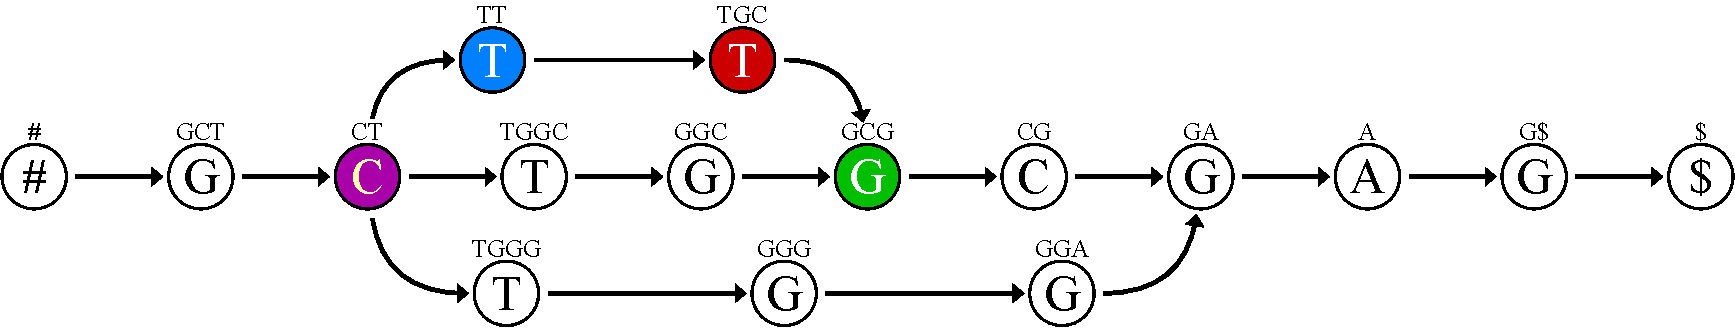
\includegraphics[width=\textwidth]{evo_fig_flat_table_with_ct.pdf}
\caption[Graph corresponding to a flat table]{Graph corresponding to flat table~\ref{table:flat_table_with_ct}. The nodes highlighted in this graph correspond to the cells highlighted in the flat table.} \label{fig:evo_fig_flat_table_with_ct}
\end{figure}
% TODO :: make sure that these two (the table and the figure) actually end up on the same page, and are not split over several pages
More formally, we can observe that 
if we have a cell in column $ i $ of the FC row, and want to find the other cells corresponding to 
the node which this cell belongs to, then we first of all check the value of $ M $ in column $ i $. 
If it is zero, we go to the left until we reach a column $ j $ which contains a one in $ M $. 
If it is not zero, then we set $ j = i $. 
We now go to the right from cell $ j + 1 $ onwards, until we encounter a one in $ M $ in column $ k $. 
This shows us that all the FC values and all the $ M $ value 
from columns $ j $ until $ k - 1 $, including both $ j $ and $ k - 1 $, 
belong to the same node in the graph. \\
To find the corresponding BWT and $ F $ values, we iterate over all columns of the table from the beginning on 
the left until we reach $ j $, and count the occurrences of ones in $ M $. 
We refer to this operation as computing the \textit{rank} of character 1 in sequence $ M $ until the limit $ j $, 
which we denote as $ \textrm{rank}_1 ( M, j ) $ \citep{Siren2009}.\label{def:rank} 
We then iterate over the columns of the table again from the beginning on the left, 
increasing a counter every time that the bit vector $ F $ contains a one, until we reach 
the result that the rank operation gave us. 
We refer to this as a \textit{select} operation, selecting character 1 in sequence $ F $ until the limit $ l $, 
where $ l $ in this case is set as the result of the rank operation before. In general, 
we denote such a select operation as $ \textrm{select}_1 ( F, l ) $ \citep{Siren2009}.\label{def:select} \\
The result of the select operation is now the index $ h $ of the column in which the BWT and $ F $ values 
of the node we are interested in start. 
We again go on to the right through $ F $ until we encounter the next one in column $ g $, 
and finally know that the node which we were interested in corresponds to the 
FC and $ M $ values in columns $ j $ until $ k - 1 $ and to the BWT and $ F $ values in columns $ h $ until $ g - 1 $. \\
Similar operations can be performed to find the range in FC and $ M $ given an index into the BWT, 
namely ranking the index in $ F $ and calling a select operation on $ M $ to find the corresponding start.

The previous approach assumed that we were given the index $ i $ of a cell in the FC row, 
and were interested in finding all other cells corresponding to the same node as that cell. 
We also mentioned a second approach based on an index of a cell in the BWT row. 
However, we can lastly introduce a more general indexing approach independent of whether we 
are considering the FC row or the BWT row. \\
The underlying insight for this third indexing method is that although the cells in the BWT 
and FC rows corresponding to a node can lie far apart, the order of nodes in both rows is exactly the same. 
More formally, if the cells corresponding to node $ u $ are sorted before the cells corresponding to node $ v $ in 
the FC row, then the cells corresponding to node $ u $ are also sorted before the cells corresponding to node $ v $ in 
the BWT, and vice versa. The reason for this to be true is that the shift in cell locations occurs due to zeroes in 
the $ M $ and $ F $ vectors, which can expand the width of an area taken up by a node, but cannot change the order 
in which the nodes are sorted. \\
Therefore, a viable method for indexing a node $ v $ in a flat table 
is to simply give an integer $ i $ corresponding to how many nodes $ u_j $ are encoded before, or to 
the left of, node $ v $. 
To find the cells in the FC row corresponding to node $ v $ we can then call $ \textrm{select}_1 ( F, i ) $ to 
find the first column and append columns while $ F $ is zero. 
To find the cells in the BWT row corresponding to node $ v $ we can call $ \textrm{select}_1 ( M, i ) $ to 
find the first column and append columns while $ M $ is zero.

Overall we now have three ways to address a node within a flat XBW table: 
We can use an integer index corresponding to a column in the FC row, 
which we will refer to as \textit{FC-indexing}\label{def:fc_indexing}, 
we can use an integer index corresponding to a column in the BWT row, 
which we will refer to as \textit{BWT-indexing}\label{def:bwt_indexing}, 
and we can use an integer index corresponding to the position of a node in the table, 
which we will refer to as \textit{absolute indexing}\label{def:absolute_indexing}. \\
As an example, we can consider the node highlighted in green in table~\ref{table:flat_table_with_ct}. 
Its FC-index is 8, as we start to count from 0 and the first green column in the FC row is in position 8. 
Its BWT-index is 7, as the first green column in the BWT row is in position 7. 
Finally, its absolute index is 6, as there are 6 nodes preceding it to the left, one 
with label “\$”, one with label “A”, two with label “C” and two with label “G”. \\
Calling $ \textrm{select}_1 ( M, 6 ) \boldsymbol{=} 8 $ gives us the FC-index from the absolute index and 
calling $ \textrm{select}_1 ( F, 6 ) \boldsymbol{=} 7 $ gives us the BWT-index from the absolute index. 
We can also call $ \textrm{rank}_1 ( M, 8 ) \boldsymbol{=} 6 $ to get the absolute index from the FC-index 
and $ \textrm{rank}_1 ( F, 7 ) \boldsymbol{=} 6 $ to get the absolute index from the BWT-index. 
Conversions from the FC-index to the BWT-index and vice versa can therefore simply be executed as conversions 
to the absolute index and back. \\
To find the FC-index at which the cells of the node end, 
we can call $ \textrm{select}_1 ( M, 6 + 1 ) - 1 \boldsymbol{=} 8 $, which 
is the same as the FC-index at which the cells of the node start, as the node 
only occupies one column in the FC row. 
To find the BWT-index at which the cells of the node end, 
we can call $ \textrm{select}_1 ( F, 6 + 1 ) - 1 \boldsymbol{=} 8 $, which 
is one more than the BWT-index at which the cells of the node start, 
as the node occupies two columns in the BWT row.

Each of the three indexing methods presented here 
may be used in practice, and choosing one of them as standard to which 
we always need to conform would create unnecessary computational effort for conversions 
between them. 
Therefore, whenever work within flat XBW tables is performed, great care must be taken 
to make clear which kind of indexing is used at each step.

We conclude the explanation of node tables and flat tables by remarking that while each column 
in an XBW node table corresponds to a node in the graph, 
each column in the flat table can be thought of as corresponding to an edge in the graph, 
if the BWT and $ F $ rows are thought of separately from the FC and $ M $ rows. 
That is, each of the columns in the BWT and $ F $ rows corresponds to an incoming edge for some node, 
and each of the columns in the FC and $ M $ rows corresponds to an outgoing edge for some node. 
Therefore, we are always assured that the total length of the BWT, $ F $, FC and $ M $ rows are the same 
within the flat table, as the total amount of outgoing edges from all nodes in the graph is 
the same as the total amount of incoming edges into all nodes in the graph.

\chapter{Methods}
% Lösungsansatz / VON UNS vorgeschlagene Methoden
%
% ====================================================================================================================================
%                                                                                                                              METHODS
% ====================================================================================================================================

To be able to understand the different existing approaches for working with 
reference graphs and genomic graphs in general, we have re-implemented several 
of these approaches myself. These implementations have been done in the programming 
language Python and resulted in several scripts that can be steered 
by a graphical main program written in Delphi. \\
We have then focused on creating the Graph Merging Library GML, which is a 
collection of algorithms written in JavaScript that make it possible to 
work with reference graphs in various ways. JavaScript is not a particularly fast 
language in itself, due to many inbuilt functionalities which are helpful for programming 
in it but slow it down compared to other languages such as C/C++ \citep{Taivalsaari2008}. 
The aim of this library is therefore not to directly provide a means to actually do 
real-world calculations using the entire human genome as reference graph, 
but instead it is focused on showing how different algorithms work, 
and in general to provide a test bed for working with genomic graphs. \\
Nevertheless, porting these algorithms to a faster programming language 
and using them in a production environment should of course be possible.

\section{Data Formats}
%
% ~~~~~~~~~~~~~~~~~~~~~~~~~~~~~~~~~~~~~~~~~~~~~~~~~~~~~~~~~~~~~~~~~~~~~~~~~~~~~~~~~~~~~~~~~~~~~~~~~~~~~~~~~~~~~~~~~~~~~~~~~~~~~~~~~~~~
%                                                                                                                METHODS: Data Formats
% ~~~~~~~~~~~~~~~~~~~~~~~~~~~~~~~~~~~~~~~~~~~~~~~~~~~~~~~~~~~~~~~~~~~~~~~~~~~~~~~~~~~~~~~~~~~~~~~~~~~~~~~~~~~~~~~~~~~~~~~~~~~~~~~~~~~~

In the course of working on this thesis we used and compared existing data 
formats for genomic graphs as well as designed several new data formats 
to be able to better understand the strengths and weaknesses of 
different possible approaches for encoding graphs.

\subsection{FASTG Format}

There are many formats readily available for genomic data strings 
that can be used when only sequential data is considered. 
One of the most common formats for genomic strings is the FASTA format \citep{Childs2007}. 
Its simple structure as a plain text format consisting of a definition line 
followed by the genomic data means that it is human-readable 
and can easily be used by various programs.

However, the aim here is to find data formats that are capable of 
encoding genomic graphs rather than strings. 
A FASTA-like format designed to handle graph data is FASTG \citep{specFASTG}. \\
This format was especially designed to enable quick conversion from a file 
encoded in FASTG back to FASTA to enable backwards compatibility with tools which cannot 
handle the graph portion of the data. In that case, all the graph portions are simply left 
out and a path through the graph becomes the genomic string encoded in the converted FASTA file. \\
In the FASTG format, genomic graphs are represented by providing the global structure of 
the data, which describes the overall structure of the entire graph, 
into which linear sequences and local graphs are embedded. 
All of this is then surrounded by specific begin and end lines which identify the file as being 
in the FASTG format. 
An example for a graph encoded in the FASTG format can be seen in figure~\ref{fig:evo_fig_fastg_example}.

% GACGT|,2,T,4 without # and $   and   AAGT|,1,,4 without # and $ (flipped arrow)
\begin{figure}[!htb]
\centering
\begin{tabularx}{1.0\textwidth}{ | X | }
\hline
\texttt{\#FASTG:begin;} \\
\texttt{\#FASTG:version=1.0:assembly\_name={\textquotesingle}example graph{\textquotesingle};} \\
\texttt{>chr1;} \\
\texttt{GA[1:alt:allele|C,T]GT} \\
\texttt{>chr2:chr2;} \\
\texttt{AAGT} \\
\texttt{\#FASTG:end;} \\
\hline
\end{tabularx}
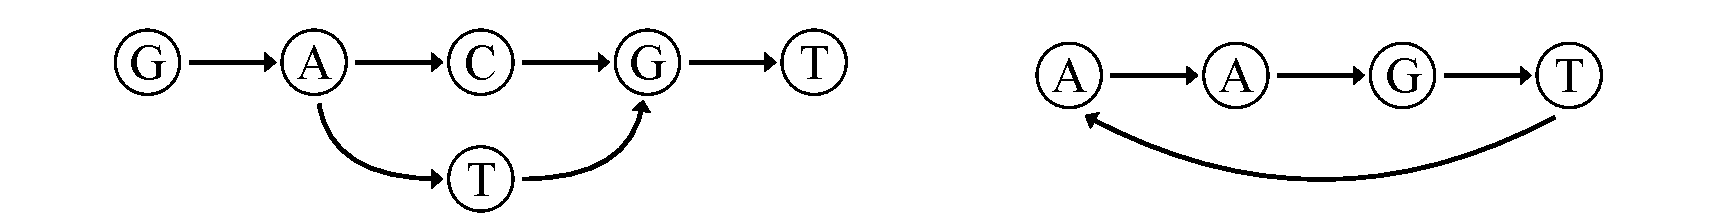
\includegraphics[width=\textwidth]{evo_fig_fastg_example.pdf}
\caption[FASTG example file]{FASTG example file together with the graph that the file represents.} \label{fig:evo_fig_fastg_example}
\end{figure}

The global structure is hereby represented by several data blocks, each of which contains 
a definition line starting with the character “$>$”, followed by one or several lines 
representing the genomic data within that block. 
The text in the definition line hereby determines how several such data blocks relate to each 
other and the global structure of the encoded data, such that a data block can represent a cycle 
or a linear part, and its ends can be attached to other data blocks. They however do not have to 
be attached to other data blocks, such that it is also possible to encode graphs in the FASTG format 
which are not connected, meaning that not all nodes within the graph need to be reachable from all other nodes. \\
The linear structure of the data is encoded via special commands right inside the data block. 
Examples for some common local commands are shown in table~\ref{table:fastg_local_examples}.

\begin{table}[htb]
\centering
\caption[Local commands in FASTG]{Examples for local commands in FASTG.}
\begin{tabularx}{1.0\textwidth}{ | l | X | }
\hline
\textbf{Example} & \textbf{Remarks} \\
\hline
\texttt{[6:gap:size=(6,4..8)]} & Gap of four to eight characters, with default gap length of six characters. \\
\hline
\texttt{[1:alt|C,CG,TT]} & Bubble representing the options of “C”, “CG” or “CT” with the default option being the first one. \\
\hline
\texttt{[1:alt:allele|A,T]} & Bubble representing the options of “A” or “T” with the default option being the first one. We use the \texttt{allele} term to denote that we are sure that both options occur in the sample data. \\
\hline
\texttt{[10:tandem:size=(5,3..7)|CG]} & Three to seven repeats of “CG”, with the default being five repeats. \\
\hline
\texttt{[20:digraph:...]} & A local graph within the format which takes up a default length of twenty characters. The actual graph definition inside the \texttt{digraph} command is replaced by “\texttt{...}” for brevity. \\
\hline
\end{tabularx}
\label{table:fastg_local_examples}
\end{table}

When referring to “default” values in this table, we mean that these are the values taken when the FASTG file 
is converted to FASTA and not the entire variety of the data can be upheld.

\subsection{GFA Format}

The GFA or Graphical Fragment Assembly format 
has been proposed in 2014 \citep{specGFA1,specGFA2}. 
This young format has a lot of advantages over FASTG, mainly 
that it is more flexible by encoding graphs of any arbitrary size without 
making a distinction between local and global graphs and that it can easier be read by programs, 
as not much emphasis is put on making it human-readable. 
Therefore, the focus can lie clearly on the needs of developers of advanced software packages, 
and on allowing them to directly store the kind of data that they encounter, 
even if it complicates the format slightly.
% TODO :: citation needed?

A file in the GFA format consists of several lines of tab-delimited plain text, with each line starting 
with a character which indicates what kind of a line this particular line is \citep{specGFAnew}. 
Figure~\ref{fig:evo_fig_gfa_example} contains an example graph encoded in the GFA format.

% ACAAGGTGTCC|,3,CG,7;,5,,9 without # and $ nodes
% H   VN:Z:1.0
% S   1   ACA
% S   2   AAG
% L   1   +   2   +   1M
% S   3   AGGT
% L   2   +   3   +   2M
% S   4   TG
% L   3   +   4   +   1M
% S   5   TCC
% L   4   +   5   +   0M
% L   2   +   5   +   0M
% S   6   CACGT
% L   1   +   6   +   2M
% L   6   +   4   +   1M
\begin{figure}[!htb]
\centering
\begin{tabularx}{1.0\textwidth}{ | X | }
\hline
\texttt{H \quad VN:Z:1.0} \\
\texttt{S \quad 1 \quad ACA} \\
\texttt{S \quad 2 \quad AAG} \\
\texttt{L \quad 1 \quad + \quad 2 \quad + \quad 1M} \\
\texttt{S \quad 3 \quad AGGT} \\
\texttt{L \quad 2 \quad + \quad 3 \quad + \quad 2M} \\
\texttt{S \quad 4 \quad TG} \\
\texttt{L \quad 3 \quad + \quad 4 \quad + \quad 1M} \\
\texttt{S \quad 5 \quad TCC} \\
\texttt{L \quad 4 \quad + \quad 5 \quad + \quad 0M} \\
\texttt{L \quad 2 \quad + \quad 5 \quad + \quad 0M} \\
\texttt{S \quad 6 \quad CACGT} \\
\texttt{L \quad 1 \quad + \quad 6 \quad + \quad 2M} \\
\texttt{L \quad 6 \quad + \quad 4 \quad + \quad 1M} \\
\hline
\end{tabularx}
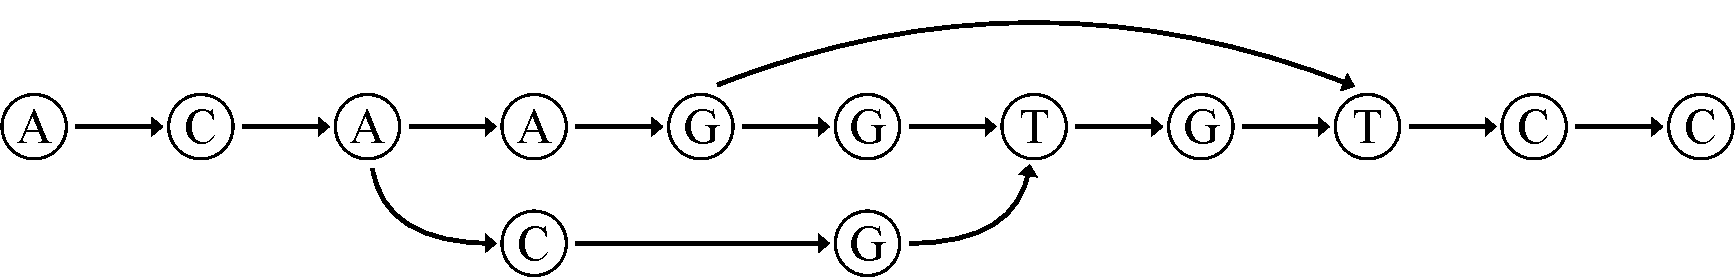
\includegraphics[width=\textwidth]{evo_fig_gfa_example.pdf}
\caption[GFA example file]{GFA example file together with the graph that the file represents.} \label{fig:evo_fig_gfa_example}
\end{figure}

The lines of the file header start with the character “\texttt{H}” and can be followed by tags which tell us about the 
version number or the quality of the data. 
Other line types include ones with character “\texttt{S}” representing sequences, which 
contain the name of the sequence and the genomic sequence itself, 
lines with character “\texttt{C}” for containments 
and lines with character “\texttt{L}”. 
These represent links between sequences which are identified by their names and orientations. 
The links are augmented by CIGAR strings. 
In general, such a CIGAR string is a sequence of lengths and operations 
associated with these lengths that is used when aligning one string to another \citep{specSAM}. 
% a really, REALLY good explanation for CIGAR strings (that I can sadly not quote as it is "just some random wiki":
% http://genome.sph.umich.edu/wiki/SAM#What_is_a_CIGAR.3F
% however, the thing that I actually am citing here (the SAM specification) is at least not too bad either,
% as it nicely defines how the CIGAR is built up
Commonly, such a string can contain the operations \texttt{M} for direct match/mismatch, 
\texttt{I} for insertions and \texttt{D} for deletions. 
However, many additional operations for skipping bases, 
clipping, padding and much more have been proposed 
for various projects \citep{specGFA1,SAM2009}.

\subsection{Bubble Format}

Having explored the FASTG and GFA format, we decided to also look 
at the bubble notation which is already partially in use within other formats, 
and base a data format solely on it. 
In other data formats, such as FASTG, bubbles are included as a way to encode very short graphs 
without the explicit generation of nodes and edges for them, 
as that would lead to a lot of overhead and decrease human-readability. 
On the other hand, adding such bubbles as options to formats which otherwise 
would already be able to contain said graphs through more complicated encoding mechanisms 
does make it more complicated for programs to work with that format, which is why the inclusion 
of such bubbles is not always seen positively \citep{specGFA1}. \\
Our format based on these bubbles 
is not supposed to be used for production environments and indeed 
is not complex enough to describe any but the most trivial kinds of graphs. 
However, we still decided to have a look into this particular format, 
as implementing it in a software package might teach us valuable lessons 
about problems to avoid when designing actual graph formats to be used for real world data.

In the bubble format a genomic sequence is represented as a single continuous string. 
There are no comments within the format, 
and neither newline characters nor in fact any kinds of whitespaces. \\
Any sort of graph representation in this format is based on bubbles, which can be extended as long as necessary, 
and can be nested. A bubble is started with a “(” character and ended 
with a “)” character. Alternatives within the bubbles are marked with “{\!\pipe}” 
characters. 
A representation of a short and simple graph in bubble notation can be seen in figure~\ref{fig:evo_fig_STPUbubble_f}.

% ACGTCTTATTTC|,4,AG,8    nicer: AG against C - CGTAGATTC|,4,C,7 (without $ and #)
\begin{figure}[!htb]
\centering
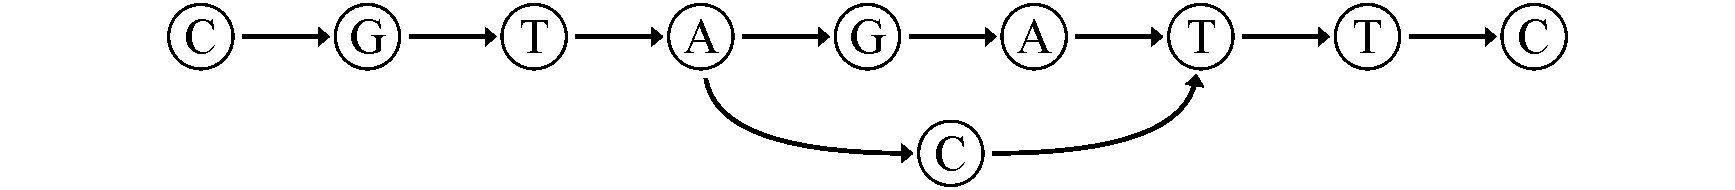
\includegraphics[width=\textwidth]{evo_fig_STPUbubble_f.pdf}
\caption[Simple bubble in bubble format]{Simple bubble, represented in bubble format as \textup{CGTA(GA\pipe C)TTC}.} \label{fig:evo_fig_STPUbubble_f}
\end{figure}

Insertions and deletions are represented as bubbles whose alternative route is empty. 
One such deletion can be seen in figure~\ref{fig:evo_fig_STPUinsertion_f}.

% ACGTATTTC|,4,AG,5    nicer: deletion - CGTAGATTC|,4,,7 (without $ and #)
\begin{figure}[!htb]
\centering

\includegraphics[width=\textwidth]{evo_fig_STPUinsertion_f.pdf}
\caption[Deletion in bubble format]{Deletion, represented in bubble format as \textup{CGTA(GA\pipe )TTC}.} \label{fig:evo_fig_STPUinsertion_f}
\end{figure}

As remarked before, this format cannot be used to represent arbitrary graphs. 
An example for which it fails to provide a correct encoding can be seen in figure~\ref{fig:evo_fig_STPUcycle_f}. 
Nevertheless, the bubble format is sufficient for simple algorithmic tests.

% CGTAGATTC|,7,,4 (without $ and #)
\begin{figure}[!htb]
\centering

\includegraphics[width=\textwidth]{evo_fig_STPUcycle_f.pdf}
\caption[Cycle in bubble format]{Cycle which cannot be fully represented in bubble format, but can be approximated to any wanted length as \textup{CGTAGAT(\pipe AGAT(\pipe AGAT(\pipe AGAT(\pipe ...))))TC}.} \label{fig:evo_fig_STPUcycle_f}
\end{figure}

\subsection{GML Format}

After implementing the Bubble Format, which represents a very straightforward but rather 
limited approach for encoding graphs, 
we decided to design a different new format to encode genomic graphs in the Graph Merging Library. 
As both the FASTG and the GFA format seem to be rather extensive, 
the idea behind the GML format is to create a simpler way of encoding graph data, 
while not falling into the pitfalls of the Bubble Format and limiting the scope of 
the graphs which could be expressed too much. 
As can be seen with the success of FASTA files for sequential data, 
the simplicity of a data format is rather important, as it makes it more likely 
for future tools to be designed with inbuilt support for the format. \\
An example graph encoded in the GML format can be seen in figure~\ref{fig:evo_fig_first_gml_example}.

% GAGTCGAT|p1,1,TGG,5;,p1:1,T,mp:6
\begin{figure}[!htb]
\centering
\begin{tabularx}{1.0\textwidth}{ | X | }
\hline
\texttt{>gml\_example\_graph} \\
\texttt{GAGTCGAT|p1,1,TGG,5;,p1:1,T,mp:6} \\
\hline
\end{tabularx}
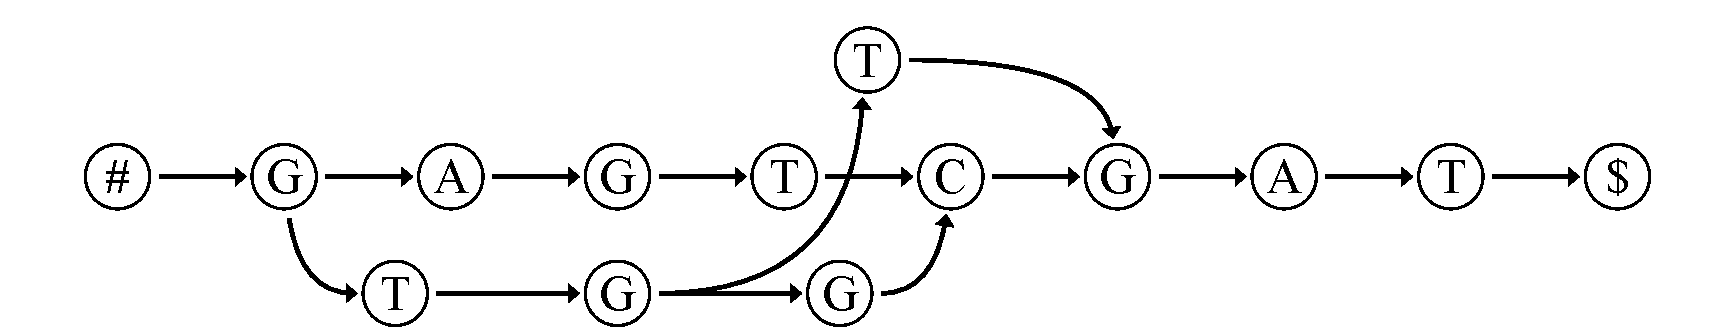
\includegraphics[width=\textwidth]{evo_fig_first_gml_example.pdf}
\caption[GML example file]{GML example file together with the graph that the file represents.} \label{fig:evo_fig_first_gml_example}
\end{figure}

An aim when designing the GML format was to not unnecessarily complicate the process of 
making existing tools of the analysis pipeline 
compatible with graph data. 
Therefore, the general structure of a GML-formatted file is similar to the general structure 
of a FASTA file, which is already widely used. \\
Namely, a GML file can contain comments and data, with different blocks of data being separated 
by comments. A comment in turn consists of the character “>” to indicate the start of a comment, 
the name of the following data block, followed by a space character and any free text that 
can be used as is deemed necessary when the file is created. 
If a GML file contains no comments at all, 
then all the rows are simply interpreted as one contiguous data block. \\
An example for how several graphs can be encoded in the GML format 
can be seen in figure~\ref{fig:evo_fig_second_gml_example}.

% CAA|,1,CG,3 and TGTC|,1,,4;,1,,3
\begin{figure}[!htb]
\centering
\begin{tabularx}{1.0\textwidth}{ | X | }
\hline
\texttt{>first\_gml\_example\_graph} \\
\texttt{CAA|,1,CG,3} \\
\texttt{>second\_gml\_example\_graph} \\
\texttt{TGTC|,1,,4;,1,,3} \\
\hline
\end{tabularx}
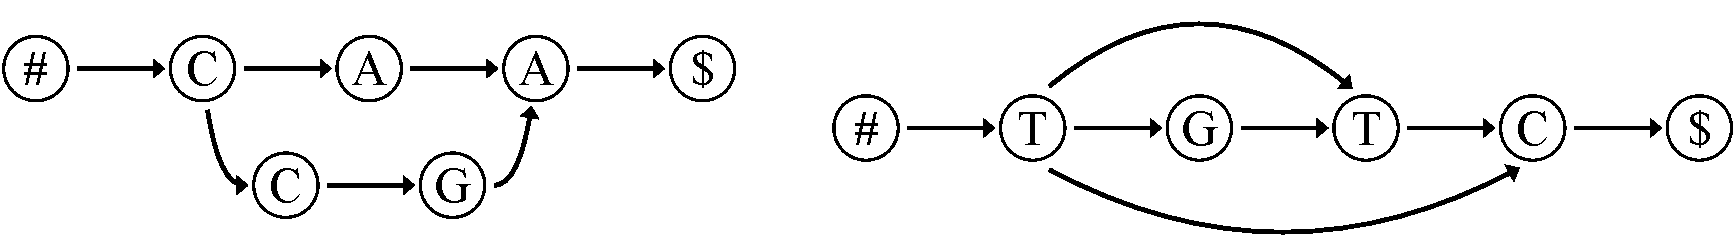
\includegraphics[width=\textwidth]{evo_fig_second_gml_example.pdf}
\caption[GML example file containing two graphs]{GML example file containing two graphs together with the graphs that the file represents.} \label{fig:evo_fig_second_gml_example}
\end{figure}

Within a data block, a genomic graph is encoded in two different parts. \\
The first part is referred to as the \textit{main path}. 
This is simply the sequence of labels on any one path from the \textit{start node}, 
which has no incoming edges, to the \textit{end node}, which has no outgoing edges. 
The start and end nodes are labelled with a hashtag symbol and a dollarsign, respectively. 
These labels are not included in the main path within the file, as they are implicitly assumed 
to exist for any such graph. \\
The second part of a data block is optional. 
If the second part is given, then the first and second part of the data block are separated by a pipe character. 
This second part is an array of info blocks, separated from each other by semicolons.

Finally, each info block consists of exactly four parts which are separated from each other by commas. \\
The first part is the identifier of the path, which can contain letters and underscores, 
as well as numbers in any position but the first. 
The identifier can also be left empty. \\
The second part is the origin of the path, 
containing the identifier of the path on which this one 
originates followed by a colon and the position within that path 
at which it originates. \\
The identifier of the main path is \texttt{mp}, but in the special case of the main path the 
identifier and the colon can be left out together, e.g. \texttt{mp:8} or just \texttt{8} for position eight 
on the main path, but \texttt{path9:8} for position eight on a path with the identifier \texttt{path9}.
Identifiers need to be defined before they can be used, that 
is, \texttt{AC|a,1,G,2;,a:0,C,3} is valid, while \texttt{AC|,a:0,C,3;a,1,G,2} is not valid. \\
The counting of the position starts at number zero for the first symbol. 
However, the main path implicitly contains the hash tag symbol and the dollar sign symbol. 
Therefore the hash tag symbol on the main path is \texttt{mp:0} and 
the first alphabetical character on the main path is \texttt{mp:1}, 
while the first alphabetical character on a path with the identifier \texttt{path9} is \texttt{path9:0}. \\
The third part is the content of the path, meaning the sequence of labels of nodes on the path. 
It can be empty if the path consists of just an edge from the origin to the target without containing any nodes. \\
The fourth part is the target of the path, 
specified according to the same format as the origin of the path in the second part of the info block.

The GML format can encode any labelled graphs which start with a special hash tag node 
and end with a dollar sign node, as long as each node within the graph 
can be reached from the start and as long as the end can be reached from 
every node as well. These constraints are acceptable for practical use, 
as nodes that cannot be reached from the start would be ignored anyway, 
as well as leaf nodes that are not the end node. \\
Despite the potential to encode such complicated structures, it is reasonably 
simple and for very short graphs even human-readable. 
With increasing graph size the readability of a GML file without special software 
decreases though, as the info blocks containing alternative paths are quite not 
located close to where they are found within the main row, but are all concentrated at the end of the file.

\subsection{FFX Format}

In the process of creating GML, we finally designed one more data format for 
genomic graphs. The idea behind FFX, the Flat Fused XBW format, is to enable saving 
a flat XBW table directly, without having to convert it to some other format 
first. \\
As shown in section~\ref{sec:fusing_flat_tables}, 
it can be helpful to fuse several separate graphs together 
instead of merging them completely. Therefore, FFX is designed 
to specifically accommodate for these kinds of fused structures as well. 
It does not however impose these fused structures on the user, 
as non-fused graphs can simply be stored as single data blocks within 
an FFX file. 
An FFX example file and the graph that it represents can be seen in figure~\ref{fig:evo_fig_ffx_example}.

% AGAgctTAC|,2,AC,6;,3,,8
\begin{figure}[!htb]
\centering
\begin{tabularx}{1.0\textwidth}{ | X | }
\hline
\texttt{>ffx\_example\_graph} \\
\texttt{B \quad CGTAG\#GAGAAATC\$} \\
\texttt{M \quad 111111111001111} \\
\texttt{F \quad 111011111011111} \\
\texttt{O \quad \$>0,A>1,C>2,G>3,T>4,\#>5} \\
\texttt{C \quad \$>0,A>1,C>6,G>8,T>12,\#>14} \\
\hline
\end{tabularx}
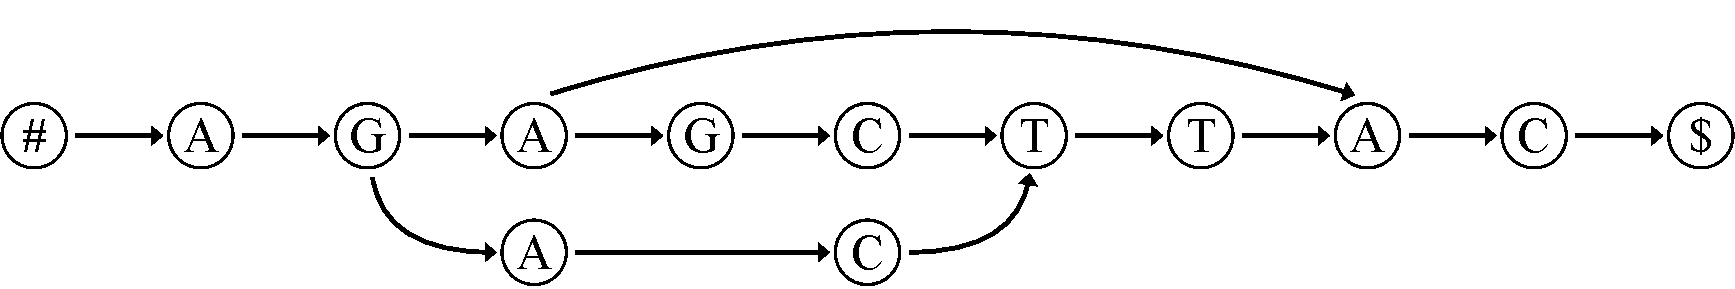
\includegraphics[width=\textwidth]{evo_fig_ffx_example.pdf}
\caption[FFX example file]{FFX example file together with the graph that is represented by the file.} \label{fig:evo_fig_ffx_example}
\end{figure}

The basic structure of an FFX file is again inspired by FASTA, 
containing an optional starting comment which contains an identifier for 
the contents of the file and other text that can be used freely. 
The optional comment is then followed by one or several data blocks, 
with each data block being separated by comment lines. \\
However, if several data blocks are included within one FFX file, 
they are not seen as separate entities. Instead, the program working on 
the FFX file is supposed to handle them as fused flat XBW tables, 
with the end node of the first table leading into the start node of the 
second table, the end node of the second leading into the start node of the 
third, and so on. 
For a more detailed explanation of how fused 
flat tables work and the motivation behind using them, 
see section~\ref{sec:fusing_flat_tables}. \\
As more complex formats are less likely to become 
used by the community at large as it would be harder to re-implement them 
in various situations, these fused data structures are required to be strictly linear. 
This means that a data block is always fused to the one directly following 
within the file. 
Just like the encoding of the global structure happens in FASTG, 
it would be possible to create a set of rules for the comment 
lines to indicate that other relations should instead take place, such as the 
end node of the first table leading to the start node of the fourth and so on, 
but even though this would increase the flexibility of the format, it would only 
increase the difficulty of writing an implementation for it. 
Likewise, each data block is only allowed to contain exactly one hash tag node 
as start and exactly one dollar sign node as end. Therefore, the path from one 
data block to the next is always completely linear, and every path through the 
entire FFX file must use every edge between the data blocks exactly once. \\
At the first glance, this might seem like a rather limiting constraint. 
However, it should be noted that much more complex behaviour is very possible 
within each data block, which can encode as complex a graph as is necessary 
as long as it does not contain any loops. 
Also, this is inspired by the actual needs for a huge graph reference, 
in which the overall structure is linear and all perturbations are on a 
rather local scale. \\
Figure~\ref{fig:evo_fig_ffx_example_fused} contains an example for 
how several graphs can be encoded in the FFX format as a single fused graph. 

% CAA|,1,G,3 and TGA|,1,,3
\begin{figure}[!htb]
\centering
\begin{tabularx}{1.0\textwidth}{ | X | }
\hline
\texttt{>first\_fused\_graph} \\
\texttt{B \quad AAGC\#C\$} \\
\texttt{M \quad 1111011} \\
\texttt{F \quad 1101111} \\
\texttt{O \quad \$>0,A>1,C>2,G>3,\#>4} \\
\texttt{C \quad \$>0,A>1,C>3,G>5,\#>6} \\
\texttt{>second\_fused\_graph} \\
\texttt{B \quad AGTT\#\$} \\
\texttt{M \quad 111101} \\
\texttt{F \quad 110111} \\
\texttt{O \quad \$>0,A>1,G>2,T>3,\#>4} \\
\texttt{C \quad \$>0,A>1,G>2,T>3,\#>5} \\
\hline
\end{tabularx}
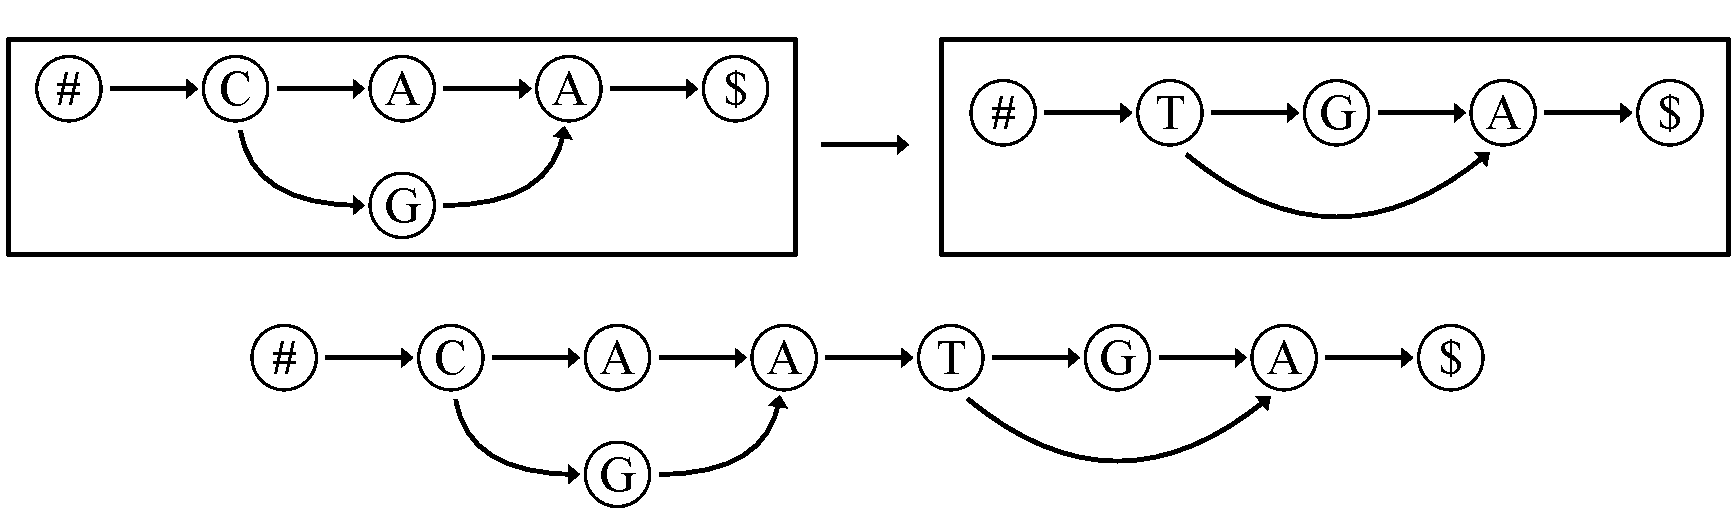
\includegraphics[width=\textwidth]{evo_fig_ffx_example_fused.pdf}
\caption[FFX example file containing fused graphs]{FFX example file containing two graphs (top) together with the fused graph that is represented by the file (middle) and the graph that the fused graph represents (bottom).} \label{fig:evo_fig_ffx_example_fused}
\end{figure}

In FFX, each data block consists of lines for the BWT, the $ M $ and $ F $ bit vectors, 
as well as lines for the ord and $ C $ arrays. 
Both of these arrays could be constructed on the fly from just the BWT. 
This however takes up a lot of time while they both only take up a small 
amount of space even for very large graphs, 
such that storing them explicitly within the file means that the 
lengthy process of computing them does not need to be repeated again and again 
whenever the file is opened. \\
In particular, the BWT is contained in a line starting with the letter “\texttt{B}” followed 
by a tab character. 
Similarly, the bit vector $ M $ is contained in a line starting with “\texttt{M}” and 
the bit vector $ F $ in a line starting with “\texttt{F}”. 
Finally, the ord and $ C $ arrays are 
contained in lines starting with “\texttt{O}” and “\texttt{C}”, respectively.

\subsection{Implementation}
%
% ~~~~~~~~~~~~~~~~~~~~~~~~~~~~~~~~~~~~~~~~~~~~~~~~~~~~~~~~~~~~~~~~~~~~~~~~~~~~~~~~~~~~~~~~~~~~~~~~~~~~~~~~~~~~~~~~~~~~~~~~~~~~~~~~~~~~
%                                                                                METHODS: Python Scripts / Data Format Implementations
% ~~~~~~~~~~~~~~~~~~~~~~~~~~~~~~~~~~~~~~~~~~~~~~~~~~~~~~~~~~~~~~~~~~~~~~~~~~~~~~~~~~~~~~~~~~~~~~~~~~~~~~~~~~~~~~~~~~~~~~~~~~~~~~~~~~~~

To compare the different data formats that have been proposed, 
we wrote several scripts in Python. 
These scripts support simplified versions of each step in a complete read alignment pipeline. 
The goal here was not to achieve a software package that could compete with 
the already commonly used alignment solutions, but rather to have a 
simple test bed for trying out different algorithmic approaches and file formats.

Section~\ref{sec:results_data_formats} contains the results gained by 
implementing the different data formats.

\section{Graph Merging Library}
%
% ~~~~~~~~~~~~~~~~~~~~~~~~~~~~~~~~~~~~~~~~~~~~~~~~~~~~~~~~~~~~~~~~~~~~~~~~~~~~~~~~~~~~~~~~~~~~~~~~~~~~~~~~~~~~~~~~~~~~~~~~~~~~~~~~~~~~
%                                                                                                       METHODS: Graph Merging Library
% ~~~~~~~~~~~~~~~~~~~~~~~~~~~~~~~~~~~~~~~~~~~~~~~~~~~~~~~~~~~~~~~~~~~~~~~~~~~~~~~~~~~~~~~~~~~~~~~~~~~~~~~~~~~~~~~~~~~~~~~~~~~~~~~~~~~~

After gathering experience on how to implement a pipeline used for aligning reads to a reference in general, 
we created the Graph Merging Library. 
\begin{figure}[!htb]
\centering
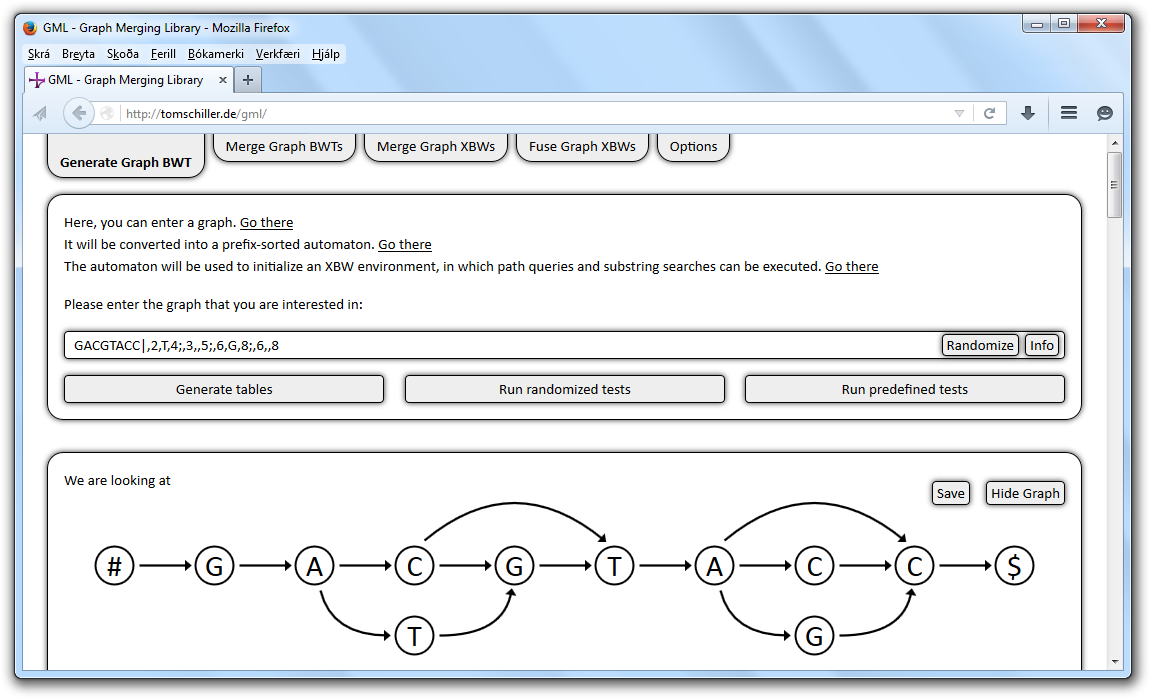
\includegraphics[width=0.95\textwidth]{evo_gml_3.png}
\caption[GUI of the Graph Merging Library]{Graphical User Interface of the Graph Merging Library.} \label{fig:evo_gml_3}
\end{figure}
This is a software library written in JavaScript, with a graphical user interface written in HTML and CSS, 
that can be used to more explicitly understand how various algorithms for working with genomic graphs work. 
A screenshot of user interface can be seen in figure~\ref{fig:evo_gml_3}. \\
In particular, GML includes different methods for merging and fusing genomic graphs, 
which may be helpful to other future projects.

\section{Core Assumptions of GML}
\label{sec:gml_core_assumptions}
%
% ~~~~~~~~~~~~~~~~~~~~~~~~~~~~~~~~~~~~~~~~~~~~~~~~~~~~~~~~~~~~~~~~~~~~~~~~~~~~~~~~~~~~~~~~~~~~~~~~~~~~~~~~~~~~~~~~~~~~~~~~~~~~~~~~~~~~
%                                                                                                     METHODS: Core Assumptions of GML
% ~~~~~~~~~~~~~~~~~~~~~~~~~~~~~~~~~~~~~~~~~~~~~~~~~~~~~~~~~~~~~~~~~~~~~~~~~~~~~~~~~~~~~~~~~~~~~~~~~~~~~~~~~~~~~~~~~~~~~~~~~~~~~~~~~~~~

There are several core assumptions which graphs need to fulfill to be used within the Graph Merging Library. 
These are chosen to simplify working on the graph as opposed to working on more general arbitrary graphs, 
while allowing for enough freedom to encode actual real world data. 
In particular, graphs considered in GML are finite automata.

\subsection{Graph Properties}

A graph $ G = (V, E) $ used in the Graph Merging Library is generally considered to consist of labelled nodes 
and directed edges, as introduced in section~\ref{sec:graph_definition}. \\
We assume that the graph is \textit{connected}. 
% GACGT|,2,T,4;,3,,5 vs. ACCTG|,1,,5;,1,,3 with no start and end nodes, and taking out the edge in the middle
\begin{figure}[!htb]
\centering
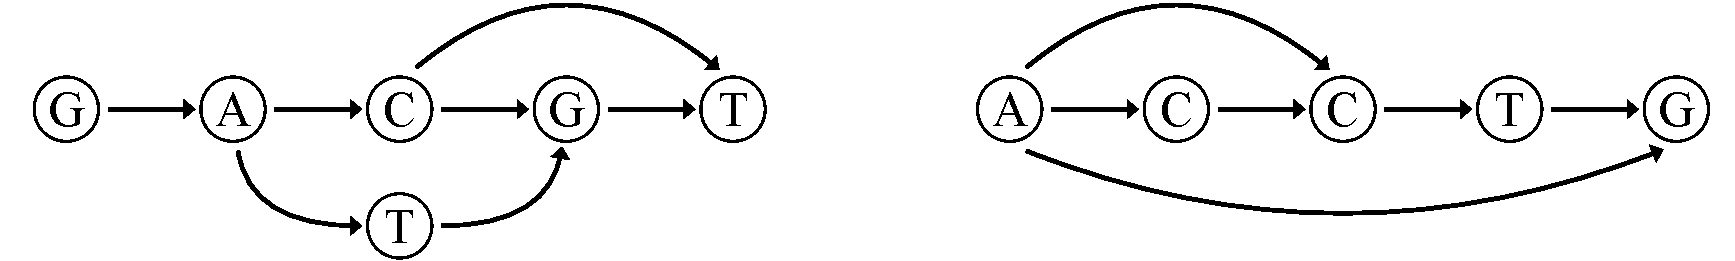
\includegraphics[width=\textwidth]{evo_fig_assume_connectedness.pdf}
\caption[Graph which is not connected]{A graph which is not connected, consisting of two clusters of nodes. The nodes within each cluster are connected among each other through edges, but are not connected to nodes of the other cluster.} \label{fig:evo_fig_assume_connectedness}
\end{figure}
We define a graph to be connected if every node of the graph is connected to every other node of the graph through some edges, 
even if not every node is reachable from every other node. This means that every 
set of two nodes needs to be connected by a series of edges, but not all of them need to face in the same direction. 
An example for a graph violating this assumption can be seen in figure~\ref{fig:evo_fig_assume_connectedness}. 
Also, the edges in the graph need to be \textit{unique}. 
% GACGTACCT|,3,,5;,6,,8 to get the arrows and then also 
\begin{figure}[!htb]
\centering
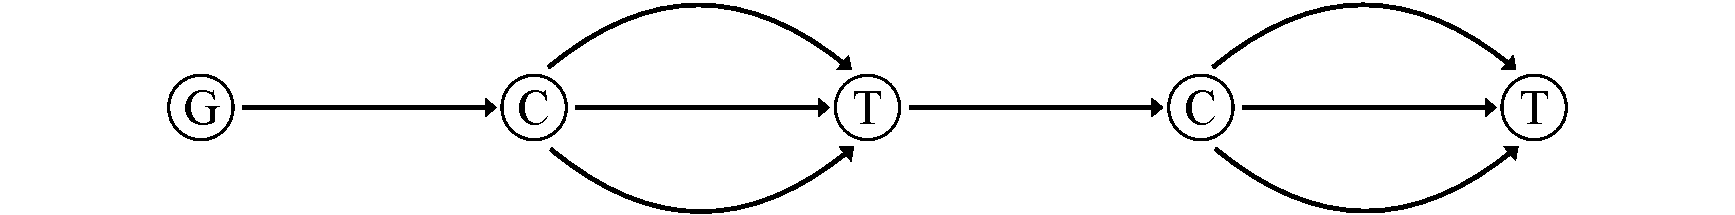
\includegraphics[width=\textwidth]{evo_fig_assume_unique_edges.pdf}
\caption[Graph with edges which are not unique]{A graph with edges which are not all unique, as there are several edges which share the same origin and target node.} \label{fig:evo_fig_assume_unique_edges}
\end{figure}
This means that no two directed edges $ (u_1, v_1) {\: \in \:} E $ and $ (u_2, v_2) {\: \in \:} E $ are allowed to 
exist within the same graph for which both $ u_1 = u_2 $ and $ v_1 = v_2 $ are true. 
A graph not obliging with this requirement is shown in figure~\ref{fig:evo_fig_assume_unique_edges}. \\
Graphs within the Graph Merging Library are supposed to be \textit{acyclic}, 
meaning that they are not allowed to contain any loops. These are paths along 
the directed edges which lead from a node onto itself, either directly or along a sequence of edges through other nodes. \\
% TODO FIGFIGFIG :: inifinite loops
The alphabet $ \Sigma $ is assumed to contain only upper case English letters for graphs within GML.

Graphs are also assumed to have exactly one \textit{start node}\label{def:start_node} $ v_s $ with the label “$\#$” which 
is the start of each path traversing the entire graph. This means that there is only one node with no incoming 
edges, this node has the label “$\#$”, and it is the only node in the graph with this label. 
The lexicographic value of the character “$\#$” is supposed to be above the 
lexicographic value of all characters in the alphabet $ \Sigma $, 
which is however not the case for “$\#$” in ASCII \citep{ASCII}. 
We therefore internally use the character “{\textasciicircum}”, whose lexicographic value encoded in ASCII 
is above all English letters in upper case. 
This is also the reason why we work with upper case letters as node labels instead of allowing lower case letters as well. 
Before being displayed, the character “{\textasciicircum}” is replaced by “$\#$”. \\
Furthermore, each graph is assumed to have exactly one \textit{end node}\label{def:end_node} $ v_e $ with the label “\$” in which 
each path traversing the entire graph ends. This can be reformulated as there being only one node without any 
outgoing edges, this node having the label “\$”, and no other node in the graph having this label. 
The lexicographic value of the character “\$” is supposed to be below the 
lexicographic value of all characters in the alphabet $ \Sigma $, 
which is the case for “\$” if the alphabet only contains English letters and the encoding in 
which string characters are compared is ASCII. \\
It should be noted that we use two different conventions concerning 
an edge from the end node $ v_e $ to the start node $ v_s $. 
When we are working with XBW node tables or with flat XBW tables, 
we assume that there is an edge leading from the end node to the start node, 
but that there still is no other incoming edge into the start node and no other outgoing edge out of the end node. 
This simplifies working with these tables slightly, as the FC row then exactly corresponds 
to the alphabetically sorted BWT row. 
If there was no such edge from $ v_e $ to $ v_s $, 
then the BWT would contain the symbol “$\#$”, but it would be missing the “\$” character. 
Also, the FC row would contain the “\$” character, but it would be missing the “$\#$”. \\
On the other hand, when we are considering graphs internally as arrays of nodes which 
each contain a label, an array of predecessors and an array of successors, 
then we explicitly assume there not to be an edge from the end node to the start node. 
This means that the predecessor array of the start node is empty, 
and the successor array of the end node is empty, 
which can be checked as alternative to reading out the label of the node and checking 
whether it is a special character.

% AtctCAG|p1,1,gg,4;PATH,2,cta,6;P2,5,T,7;,P1:1,,P2:0
\begin{figure}[!htb]
\centering
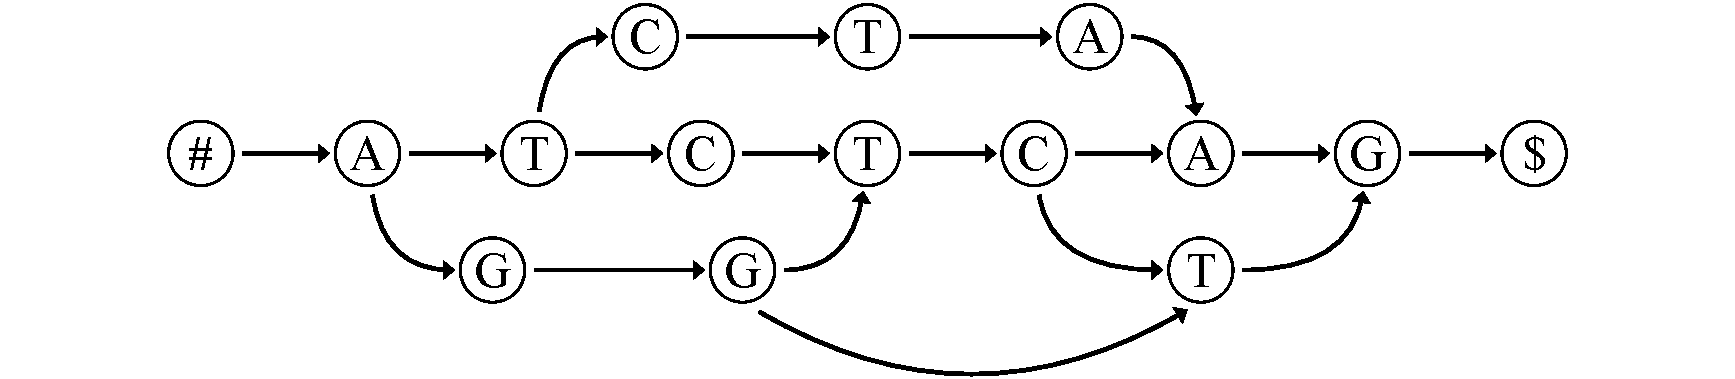
\includegraphics[width=\textwidth]{evo_fig_assume_all_good.pdf}
\caption[Graph fulfilling core assumptions of GML]{A graph fulfilling the core assumptions of GML.} \label{fig:evo_fig_assume_all_good}
\end{figure}

A graph which is not violating any of aforementioned assumptions can be seen in figure~\ref{fig:evo_fig_assume_all_good}.

\subsection{Additional Assumptions for Merging Graphs}

If graphs are supposed to be merged together, then another core assumption is added, 
which states that no node splitting is allowed to be needed between these graphs. 
That is, at no point within the merging process shall it be necessary to 
connect the two graphs through more than one edge.
% informally, we refer to this scenario as "splitover"

% TODO FIGFIGFIG :: show an image of a splitover - several edges connecting this and that, etc. bla blubb

In addition to this extra requirement, we also take care with the end node of the first graph 
to be merged and the start node of the second graph, as these are special nodes which will be 
deleted after the merging has been finished. \\
Just as with “$\#$”, which encoded in ASCII does not have the lexicographical properties 
that we require, we also replace two other special characters internally with different characters. 
These are “$\$_0$” and “$\#_0$”, which we use while merging graphs. 
In particular, we sometimes replace the label of the end node of the first input graph 
with “$\$_0$” and the label of the start node of the second input graph with “$\#_0$”, 
to better be able to distinguish them from the start and end nodes of the merged graph. 
However, we need to encode them as single characters when working with flat tables 
which do not allow some cells to have different lengths. 
Therefore, we internally encode “$\$_0$” as the percent sign “\%” and 
we internally encode “$\#_0$” as the underscore sign “\_”. \\
A clear lineup of all special characters which we use in GML can be found in table~\ref{table:special_characters}.
\begin{table}[htb]
\centering
\caption[Special characters in GML]{Special characters in GML together with information about how they are encoded internally as well as remarks about their use.}

\begin{tabular}{ | c | c | l | }
\hline
\textbf{Character} & \textbf{Encoded as} & \textbf{Remarks} \\
\hline
\$ & \$ & label of the end node $ v_e $ \\
\hline
$\#$ & {\textasciicircum} & label of the start node $ v_s $ \\
\hline
$\$_0$ & \% & label of the end node of the first input graph \\
\hline
$\#_0$ & \_ & label of the start node of the second input graph \\
\hline
! & ! & error character during prefix generation \\
\hline
\end{tabular}

\label{table:special_characters}
\end{table}

\section{Generating a Genomic Graph}
%
% ~~~~~~~~~~~~~~~~~~~~~~~~~~~~~~~~~~~~~~~~~~~~~~~~~~~~~~~~~~~~~~~~~~~~~~~~~~~~~~~~~~~~~~~~~~~~~~~~~~~~~~~~~~~~~~~~~~~~~~~~~~~~~~~~~~~~
%                                                                                                  METHODS: Generating a Genomic Graph
% ~~~~~~~~~~~~~~~~~~~~~~~~~~~~~~~~~~~~~~~~~~~~~~~~~~~~~~~~~~~~~~~~~~~~~~~~~~~~~~~~~~~~~~~~~~~~~~~~~~~~~~~~~~~~~~~~~~~~~~~~~~~~~~~~~~~~

To use a genomic graph in the Graph Merging Library, 
a GML file can be opened which contains the desired graph, 
a valid GML data block can be entered directly into an input field, 
or a graph can be created randomly for testing purposes.

\subsection{Randomly Generating New Graphs}

The Graph Merging Library contains the function \texttt{generateRandomGraphString} for 
the automatic generation of random graphs, which can be used to quickly generate input for testing the 
provided merging functions. 
This function can be called without any arguments, in which case it will generate short graphs 
or strings. If necessary, the length of the main row can however also be provided to generate 
graphs of different lengths. The alphabet can also be specified, which otherwise will be 
set to $ \Sigma = \{ \textrm{A, C, G, T} \} $. Finally, two thresholds with values between $ 0\% $ and $ 100\% $ can 
be specified, which tell the function how likely it is to add at least one infoblock to the graph, 
and how likely it is to add more infoblocks after adding the first.

% TODO :: add more text

\subsection{Internal Graph Format}
\label{sec:internal_graph_format}

When a GML file is being opened, then some work still needs to be undertaken 
to convert the opened graph into the extended XBW format, and the graph is stored 
in a different format internally at first before this conversion occurs. \\
That is, each graph is stored as array which contains all nodes as elements. 
Every node here is an object which has the properties \texttt{c}, \texttt{n}, \texttt{p} and 
possibly \texttt{f}. The \texttt{c} property contains one character, which is the label of the node. 
The \texttt{f} property, if it is defined, contains the prefix of the node. Until the prefixes have 
been calculated, these properties can be missing. \\
The \texttt{n} property contains an array of integers, with each integer being the index 
of a node in the array representing the graph. It represents a list of all succeeding nodes. 
Similarly, the \texttt{p} property is a list of preceding nodes, implemented as array of integers, 
with each integer again being the index of a preceding node in the graph array. \\
The start node with label “$\#$” is assumed to be found as the first element 
of the graph array. Apart from this node, the positions of the other nodes within 
the array are not significant. In fact, elements of the array are also allowed to 
be empty or the boolean value \texttt{false}. This is helpful when deleting 
nodes from the graph, as the nodes with higher indices therefore do not need to be re-indexed, 
which would entail a lot of work as then all the arrays of preceding and succeeding nodes 
also would need to be updated accordingly. 
Therefore, every loop iterating over the nodes of the graph needs to check for the 
current node to actually exist before performing any work on it.

The extended XBW format requires for each graph for start with a node labelled with a 
hash tag sign and to end with a node labelled with a dollar sign, 
but these nodes are not explicitly encoded in the GML format.
Therefore, the extra node with the $\#$ label is created first when opening a GML file. 
The main row as specified in the GML file is then added as one possible way 
of traversing the graph from the $\#$ node to the \$ node, which is added at the end of the main row. \\
Finally, the info blocks are iterated over, and their contents are added as edges and nodes which are part 
of paths off the main row.
% TODO :: add algorithm: The entire process is illustrated in algorithm~\ref{alg:...}.

\section{Sanitizing the Graph}

If graphs which are used as inputs for the GML merging conform to the assumptions 
stated in section~\ref{sec:gml_core_assumptions}, 
then they can be worked on and results can be given out. 
However, in case of inputs not conforming to these assumptions, the results of the GML algorithms 
are not useful or even no results are given out, as infinite loops are encountered. 
Therefore, a sanitization step is used to ensure that the input actually conforms to the 
stated assumptions. If this is not the case, which can happen for randomly created input graphs, 
then a warning is given out telling the user that invalid input was encountered and 
no attempt is being made to actually perform work on the graph.

To perform this check of the core assumptions, the function \texttt{sanitizeAutomaton} is called within GML 
whenever an input graph string is newly converted to an internal automaton data structure representing it. 
It in turn calls several functions which check one assumption at a time. \\
The first one of these functions is called \texttt{eliminateMultipleEdgesInAutomaton}. 
Its underlying functionality can be found in algorithm~\ref{alg:eliminateMultipleEdgesInAutomaton}.
\begin{algorithm}
\caption[Unify multiple edges in a graph]{Unify multiple edges in a graph.}
\addtocontents{loa}{\vskip 15pt}
\label{alg:eliminateMultipleEdgesInAutomaton}
\begin{algorithmic}[1]
\ForAll {graph.nodes \textbf{as} node}
	\If {$ \textrm{\textbf{length of} node.predecessors} > 1 $}
	\Comment{Unify array of preceding nodes}
		\State $ \textrm{new\_array} \gets [ \, ] $
		\ForAll {node.predecessors \textbf{as} predecessor}
			\If {\textbf{not} ( new\_array \textbf{contains} predecessor )}
				\State \textbf{append} predecessor \textbf{to} new\_array
			\EndIf
		\EndFor
		\State $ \textrm{node.predecessors} \gets \textrm{new\_array} $
	\EndIf
	
	\If {$ \textrm{\textbf{length of} node.successors} > 1 $}
	\Comment{Unify array of succeeding nodes}
		\State $ \textrm{new\_array} \gets [ \, ] $
		\ForAll {node.successors \textbf{as} successor}
			\If {\textbf{not} ( new\_array \textbf{contains} successor )}
				\State \textbf{append} successor \textbf{to} new\_array
			\EndIf
		\EndFor
		\State $ \textrm{node.successors} \gets \textrm{new\_array} $
	\EndIf
\EndFor
\end{algorithmic}
\end{algorithm}
It ensures that each edge is unique, meaning that there is no pair of 
edges $ (u_1, v_1) {\: \in \:} E $ and $ (u_2, v_2) {\: \in \:} E $ for which both $ u_1 = u_2 $ and $ v_1 = v_2 $ are true. 
It does not actually throw an error if such edges are encountered, but simply deletes one edge of the pair, until none 
of these pairs of edges are left. \\
The next function is \texttt{checkAutomatonForLoops}. 
Its general approach is shown in algorithm~\ref{alg:checkAutomatonForLoops}.
\begin{algorithm}
\caption[Check if graph contains loops]{Check if a graph contains loops.}
\addtocontents{loa}{\vskip 15pt}
\label{alg:checkAutomatonForLoops}
\begin{algorithmic}[1]
\State $ \textrm{paths} \gets [ \, [ \, 0 \, ] \, ] $
\While {$ \textrm{\textbf{length of} paths} > 0 $}
	\ForAll {paths \textbf{as} path}
		\State $ \textrm{current\_node} \gets \textrm{\textbf{last element of} path} $
		\If {$ \textrm{\textbf{length of} current\_node.successors} > 0 $}
			\ForAll {current\_node.successors \textbf{as} successor}
				\If {path \textbf{contains} successor}
					\State \Return true
					\Comment{Same node encountered twice}
				\EndIf

				\If {\textbf{last iteration within this for loop}}
					\State \textbf{append} successor \textbf{to} path
				\Else
					\State $ \textrm{next\_path} \gets \textrm{path} $
					\State \textbf{append} successor \textbf{to} next\_path
					\State \textbf{append} next\_path \textbf{to} paths
				\EndIf
			\EndFor
		\Else
			\State \textbf{delete} path \textbf{from} paths
			\Comment{Drop the path if \$ node was reached}
		\EndIf
	\EndFor
\EndWhile
\State \Return false
\end{algorithmic}
\end{algorithm}
This function traverses all paths through the graph, starting from the start node, 
and checks for each new node added to a path if that node has already been traversed within the path before. 
If such a node is encountered which is traversed several times within one path, then an 
error is given out and the invalid input warning is displayed to the user. \\
Finally, the function \texttt{checkAutomatonForIncorrectChars} as shown in 
automaton~\ref{alg:checkAutomatonForIncorrectChars} iterates over all nodes of the automaton 
\begin{algorithm}
\caption[Check if graph labels contain invalid characters]{Check if graph labels contain invalid characters.}
\addtocontents{loa}{\vskip 15pt}
\label{alg:checkAutomatonForIncorrectChars}
\begin{algorithmic}[1]
\ForAll {graph.nodes \textbf{as} node}
	\If {( node.label {\boldmath$ = $} \$ ) \textbf{and} ( \textbf{length of} node.successors {\boldmath$ = $} 0 ) }
		\State \textbf{continue}
	\EndIf
	
	\If {( node.label {\boldmath$ = $} $\#$ ) \textbf{and} ( \textbf{length of} node.predecessors {\boldmath$ = $} 0 ) }
		\State \textbf{continue}
	\EndIf
	
	\If {( $ \textrm{node.label \textbf{in}} \, [ \textrm{A \textbf{to} Z} ] $ ) and ( \textbf{length of} node.label {\boldmath$ = $} 1 )}
		\State \textbf{continue}
	\EndIf
	
	\State \Return true
\EndFor
\State \Return false
\end{algorithmic}
\end{algorithm}
and checks if the labels conform to the assumptions, meaning that every node needs to have a 
label with exactly one English upper case letter, except for the start node which has the label “$\#$” and 
the end node which has the label “\$”. 
Again, if a node is encountered which does not conform to these assumptions, then the invalid input message 
is shown to the user and the computation is stopped. \\
We could also use some function to check if the graph is connected, 
but this is actually not necessary, as the GML format in which we open the graph can only encode connected 
graphs anyway. The reason for this is that a graph encoded in GML is encoded as a main path, 
together with other paths originating and terminating on the already existing paths. 
Therefore, no path can be encoded which is separate from the others, and checking afterwards if 
the emerging graph is connected becomes unnecessary.
% TODO :: add algorithms for all these!

\section{Visualizing the Graph}
%
% ~~~~~~~~~~~~~~~~~~~~~~~~~~~~~~~~~~~~~~~~~~~~~~~~~~~~~~~~~~~~~~~~~~~~~~~~~~~~~~~~~~~~~~~~~~~~~~~~~~~~~~~~~~~~~~~~~~~~~~~~~~~~~~~~~~~~
%                                                                                                       METHODS: Visualizing the Graph
% ~~~~~~~~~~~~~~~~~~~~~~~~~~~~~~~~~~~~~~~~~~~~~~~~~~~~~~~~~~~~~~~~~~~~~~~~~~~~~~~~~~~~~~~~~~~~~~~~~~~~~~~~~~~~~~~~~~~~~~~~~~~~~~~~~~~~

After opening the graph, it can be helpful to show it to the user for 
quick and easy visual inspection. 
We therefore included a small visualization function within the Graph Merging Library, 
which is capable of displaying simple graphs nicely. 
Algorithm~\ref{alg:visualize} shows how this function works in general. 
\begin{algorithm}
\caption[Visualize a graph]{Visualize a graph by first displaying one path from 
the starting node to the end node, referred to as main row, 
and then adding alternative paths around the established core.}
\addtocontents{loa}{\vskip 15pt}
\label{alg:visualize}
\begin{algorithmic}[1]
\State $ \textrm{current\_node} \gets \textrm{graph}[0] $
\Comment{Display main row}
\State \textbf{draw} current\_node
\State $ \textrm{more\_nodes} \gets [ \, ] $
\While {current\_node.label \textbf{is not} \$}
	\State \textbf{append} current\_node \textbf{to} more\_nodes
	\State $ \textrm{current\_node} \gets \textrm{current\_node.successors}[0] $
	\State \textbf{draw} current\_node
\EndWhile
\State \phantom{emptyline}
\ForAll {more\_nodes \textbf{as} path \$}
\Comment{Display other paths}
	\State $ \textrm{current\_node} \gets \textrm{path} $
	\If {current\_node has not been drawn}
		\State $ \textrm{node} \gets \textrm{current\_node} $
		\State $ \textrm{path} \gets [ \, ] $
		\While {node has not been drawn}
			\State \textbf{append} node \textbf{to} path
			\State $ \textrm{node} \gets \textrm{node.successors}[0] $
			\If {node has not been in more\_nodes before}
				\State \textbf{append} node \textbf{to} more\_nodes
			\EndIf
		\EndWhile
		\State \textbf{draw} nodes \textbf{in} path together
	\EndIf
	\ForAll {current\_node.predecessors \textbf{as} predecessor}
		\State \textbf{draw} edge \textbf{from} predecessor \textbf{to} current\_node
	\EndFor
\EndFor
\end{algorithmic}
\end{algorithm}
Having a closer look at line 1 of the algorithm, 
it can be seen that it constructs the main row 
by starting in the first node, which is assumed to 
be labelled with the hash tag symbol. 
In line 6 of the algorithm it can then be seen 
that to construct the main row starting with this node, 
the algorithm always jumps into the first of the successors of the current node. \\
Therefore, before a graph can be passed to the visualization function, 
it needs to be ensured that its hash tag node is stored in the very first position 
and that the node labelled with the dollar sign can be reached by always travelling 
along the first of the successors. 
A separate function called \texttt{makeAutomatonPretty} is used to ensure that this is always the case, 
by traversing all possible paths and picking one path which leads to the dollar sign node. 
In the options it can be chosen whether this function 
should find one of the shortest paths, which is faster, or one of the longest paths, 
which leads to a better visualization. 
When it is instructed to find one of the longest paths, it will however still ignore 
paths including loops, as it might otherwise be trapped in the loop indefinitely, 
trying to find yet longer paths. 
An example for how this choice affects 
the visualized graph can be seen in figure~\ref{fig:evo_fig_visualize_short_vs_long}.  
% merge GACGT|,2,T,4;,3,,5 vs. ACCT|,1,,4;,1,,3, once with normal settings, once with forcing shortest path
\begin{figure}[!htb]
\centering
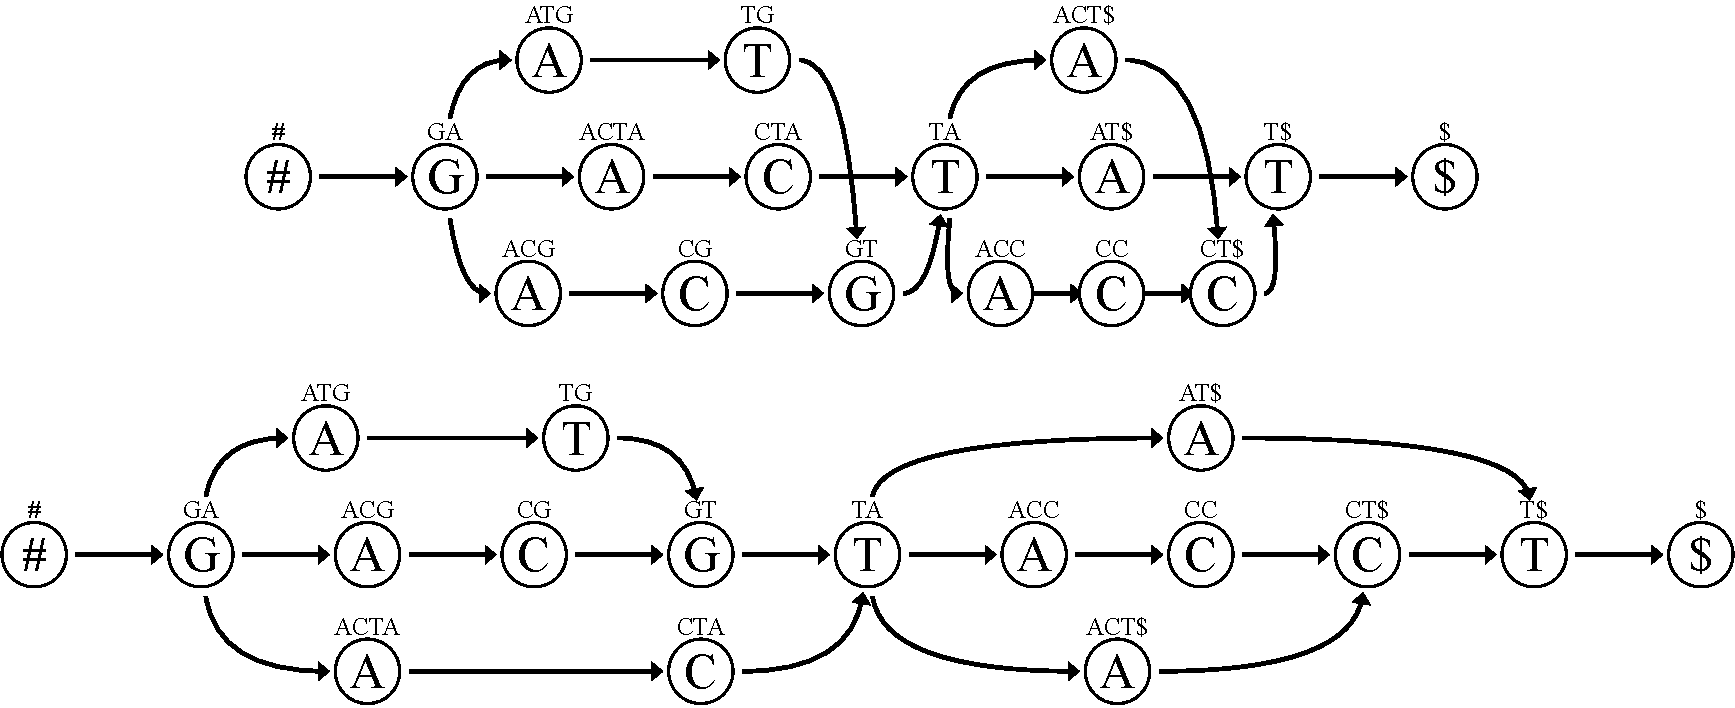
\includegraphics[width=\textwidth]{evo_fig_visualize_short_vs_long.pdf}
\caption[Visualizations of graph with shortest and longest main rows]{Two visualizations of the same graph. The visualization on the top uses the shortest possible path as main row, while the visualization on the bottom uses the longest possible path.} \label{fig:evo_fig_visualize_short_vs_long}
\end{figure}
The graph nodes are then adjusted in such a way that following the first successor of each 
node upon starting at the hash tag node leads directly to the dollar sign node. \\
It is also notable how exactly the iteration over the nodes works out. 
In line 10 we iterate over all nodes that have been added to more\_nodes, 
an array which keeps track of nodes which we have not fully worked on yet. 
This means that we may have already drawn the node, but we have not yet 
drawn all the incoming edges, and we may possibly not even have drawn the node itself. 
The loop in line 15 then iterates over all the first successors of that node, 
and adds them to an array called path, until a node is encountered that has already been drawn. 
Finally, in line 22, the entire path is drawn together. \\
Algorithmically it would be much more straightforward to simply iterate over all nodes 
and draw them when we encounter them, but in that case we would not have a good idea about 
where it might make sense to draw them. The approach of iterating over nodes 
that have not been worked on and nesting into this an iteration of the successors of that node 
allows us to instead draw entire parts of paths at once, so that we have a good idea 
where exactly to put the nodes on the display when drawing them, as they can simply 
be arranged next to each other.

\section{Direct Graph Merging}
\label{sec:direct_graph_merging}

The aim of the Graph Merging Library is to provide advanced algorithms 
for the direct merging of flat XBW tables. 
However, it is helpful to be able to quickly check whether this merging of tables 
was successful. 
We therefore developed the function \texttt{mergeAutomata}, 
the general approach of which is shown in algorithm~\ref{alg:mergeAutomata}. 
\begin{algorithm}
\caption[Merge two graphs]{Merge two graphs in a simple manner. The input consists of graph\_1 and graph\_2, which are to be merged.}
\addtocontents{loa}{\vskip 15pt}
\label{alg:mergeAutomata}
\begin{algorithmic}[1]

\State {$ \textrm{graph} \gets [ \, ] $}
\State {$ \textrm{offset} \gets ( \textrm{\textbf{length of} graph\_1} ) - 2 $}
\State {$ \textrm{into\_2} \gets \textrm{graph\_2$[ 0 ]$.n} $}

\State \phantom{nl}

\For {$ i $ \textbf{from} 0 \textbf{to length of} graph\_1}
\Comment{Start to build graph as copy of graph\_1}
	\If{graph\_1$[ i ]$.c {\boldmath$ = $} \texttt{\textquotesingle}\$\texttt{\textquotesingle}}
		\State {$ \textrm{del\_i} \gets i $}
		\State {$ \textrm{out\_of\_1} \gets \textrm{graph\_1$[ i ]$.p} $}
	\Else
		\State \textbf{append} graph\_1$[ i ]$ \textbf{to} graph
	\EndIf
\EndFor

\State \phantom{nl}

\For {$ i $ \textbf{from} 0 \textbf{to length of} out\_of\_1}
\Comment{Take out link to \$}
	\State {\textbf{delete} del\_i \textbf{from} graph$ [ \textrm{out\_of\_1$[ i ]$} ] $.n}
\EndFor

\State \phantom{nl}

\For {$ i $ \textbf{from} 0 \textbf{to length of} graph}
\Comment{Update indices after deleting \$ node}
	\For {$ j $ \textbf{from} 0 \textbf{to length of} graph$[ i ]$.p}
		\If{graph$[ i ]$.p$[ j ]$ {\boldmath$ \geq $} del\_i}
			\State {\textbf{decrease} graph$[ i ]$.p$[ j ]$}
		\EndIf
	\EndFor
	\State \textbf{Repeat previous five lines with} .n \textbf{instead of} .p
\EndFor

\State \phantom{nl}

\For {$ i $ \textbf{from} 1 \textbf{to length of} graph\_2}
\Comment{Add all nodes from graph\_2}
	\For {$ j $ \textbf{from} 0 \textbf{to length of} graph\_2$[ i ]$.p}
		\State {$ \textrm{graph\_2$[ i ]$.p} \gets \textrm{graph\_2$[ i ]$.p} + \textrm{offset} $}
	\EndFor
	\State \textbf{Repeat previous three lines with} .n \textbf{instead of} .p
	\State \textbf{append} graph\_2$[ i ]$ \textbf{to} graph
\EndFor

\State \phantom{nl}

\For {$ i $ \textbf{from} 0 \textbf{to length of} into\_2}
\Comment{Take out link to $\#$}
	\State {$ \textrm{into\_2$[ i ]$} \gets \textrm{into\_2$[ i ]$} + \textrm{offset} $}
	\State {\textbf{delete} offset \textbf{from} graph[into\_2$[ i ]$ \, ].p}
\EndFor

\State \phantom{nl}

\For {$ i $ \textbf{from} 0 \textbf{to length of} out\_of\_1}
\Comment{Attach end of graph\_1}
	\For {$ j $ \textbf{from} 0 \textbf{to length of} into\_2}
	\Comment{to start of graph\_2}
		\State {\textbf{append} into\_2$[ j ]$ \textbf{to} graph[out\_of\_1$[ i ]$.n}
		\State {\textbf{append} out\_of\_1$[ i ]$ \textbf{to} graph[into\_2$[ j ]$.p}
	\EndFor
\EndFor

\end{algorithmic}
\end{algorithm}
It is used to merge two input graphs which are stored in the internal graph format 
outlined in section~\ref{sec:internal_graph_format}. \\
The function operates by first copying every node from graph\_1 into the newly created graph, 
except for the end node with label “\$”. A list of all nodes which have outgoing edges leading to that node 
is hereby stored in the array out\_of\_1. 
This array is then iterated over, and from each of these nodes the edge leading to the end node is taken out. 
Finally, all nodes are iterated over and their pointers in the .p and .n arrays are updated to reflect 
the new positions of the nodes in the graph array which follow the now deleted end node. 
This concludes the deletion of the node with label “\$” from the first graph. \\
Most of the nodes from the second input, graph\_2, are then added to the resulting graph. 
Only one of the nodes from graph\_2 is left out, which is the start node with label “\#”. 
As the start node is defined to always be in position 0 in the graph array, 
this can simply be done by starting the iteration at position 1. 
While adding the new nodes to the resulting graph, 
all their .p and .n arrays are updated using an offset. 
This is necessary as they get appended to the end of the new graph 
and therefore their positions are different than they were in graph\_2. 
Equivalently to the array out\_of\_1, which kept track of the nodes with edges leading towards the end node in graph\_1, 
we now also use an array into\_2, which keeps track of the nodes with edges coming in from the start node in graph\_2. 
Again, these edges are deleted to fully delete the start node from graph\_2. \\
Having deleted both the end node of graph\_1 and the start node of graph\_2, 
we then attach the end of graph\_1 to the start of graph\_2, again using the out\_of\_1 and into\_2 arrays 
which tell us which nodes lie at the end of graph\_1 and at the start of graph\_2, respectively. 
This concludes the function, as the merged graph has been fully formed.

Using this function to merge the graphs directly 
enables us to generate a flat XBW table based on the merged graph, 
which can then later on be compared against the results of the 
advanced XBW table merging algorithms to check whether they successfully merged the individual tables.

\section{Ensuring the Graph is Reverse Deterministic}
\label{sec:why_rev_det}
%
% ~~~~~~~~~~~~~~~~~~~~~~~~~~~~~~~~~~~~~~~~~~~~~~~~~~~~~~~~~~~~~~~~~~~~~~~~~~~~~~~~~~~~~~~~~~~~~~~~~~~~~~~~~~~~~~~~~~~~~~~~~~~~~~~~~~~~
%                                                                                 METHODS: Ensuring the Graph is Reverse Deterministic
% ~~~~~~~~~~~~~~~~~~~~~~~~~~~~~~~~~~~~~~~~~~~~~~~~~~~~~~~~~~~~~~~~~~~~~~~~~~~~~~~~~~~~~~~~~~~~~~~~~~~~~~~~~~~~~~~~~~~~~~~~~~~~~~~~~~~~

Before being able to encode the graph as either XBW node table or as flat XBW table, 
it should be ensured that it actually is reverse deterministic.

For any node within the graph, we can construct a prefix, 
which is the sequence of its own label concatenated with the labels of the nodes which are 
traversed when exiting that node. 
% TODO :: insert image about prefixes and how they are generated 
% (even through strands that are split apart, but have identical labels)
The extended XBW compression scheme for graphs as proposed by \citet{Siren2014} relies 
on the possibility of ordering all nodes of a graph alphabetically, based on their prefixes. 
After opening a file format that can contain arbitrary graphs, 
it is therefore first of all necessary to ensure the graph is reverse deterministic, 
as otherwise at least two nodes could not be unambiguously sorted against each other. 
File formats which can contain graphs which are not reverse deterministic include 
FASTG, GFA, GML and the bubble format, while the FFX format guarantees that 
the stored data is reverse deterministic as its entire encoding paradigm 
otherwise would not work. \\
% TODO :: insert figure in which we can see a non-reverse deterministic graph and the prefixes being the same.
To understand why a graph not being reverse deterministic would lead to 
at least two nodes not being able to be unambiguously sorted by their prefixes, 
we can recall the definition of a reverse deterministic graph:

% \begin{moyadef}
\textbf{Definition} A graph is \textit{reverse deterministic} if and only if each node has no two predecessors with the same label.
% \end{moyadef}

% What we want to prove is the following theorem.
% \begin{moyatheorem}
% If a graph is not reverse deterministic, 
% then at least two of its nodes cannot be unambiguously sorted against each other.
% \end{moyatheorem}
% \begin{proof}
From the definition it can be seen that a graph $ G = (V, E) $ not being reverse deterministic means that there 
is a node $ u {\: \in \:} V $ which has at least two predecessors $ v $ and $ w $ which share a label. 
As $ v $ and $ w $ share a label, their prefixes both start with the same label. \\
Without loss of generality we can now focus on one of the two nodes $ v $ and $ w $. 
As $ v $ is a predecessor of $ u $, we can see that the 
prefix of $ v $ either continues with the prefix of $ u $, 
or that it will not be able to continue after the first character 
as there is another successor of $ v $ which has a different label than $ u $ does. \\
The same holds true for $ w $, such that both $ v $ and $ w $ have labels starting 
with the same character and are of length 1 unless they are that character concatenated 
with the prefix of $ u $. \\
Now, in case of one of the prefixes just having length 1, we cannot sort $ v $ and $ w $ 
unambiguously, as their prefixes are the same for all given characters. 
On the other hand, if both prefixes have length above 1, then they are both 
the same character concatenated with the prefix of $ u $, as we can again not sort $ v $ and $ w $ 
unambiguously. 
Therefore, a reverse deterministic graph invalidates the assumption that we can sort 
all of its nodes unambiguously alphabetically by its prefixes. \qed
% \end{proof}

The program therefore first needs to check if the opened graph is reverse deterministic. 
This can easily done by comparing the labels of every nodes' predecessors, as can be seen 
in algorithm~\ref{alg:isAutomatonReverseDeterministic}.

\begin{algorithm}
\caption[Check if a graph is reverse deterministic]{Checks if a graph is reverse deterministic.}
\addtocontents{loa}{\vskip 15pt}
\label{alg:isAutomatonReverseDeterministic}
\begin{algorithmic}[1]
\ForAll {graph.nodes \textbf{as} node}
	\State $ \textrm{encountered\_characters} \gets [ \, ] $
	\ForAll {node.predecessors \textbf{as} predecessor}
		\If {encountered\_characters \textbf{contains} predecessor.label}
			\State \Return false
		\Else
			\State \textbf{append} predecessor.label \textbf{to} encountered\_characters
		\EndIf
	\EndFor
\EndFor
\State \Return true
\end{algorithmic}
\end{algorithm}

If the graph is found not to be reverse deterministic, then it needs to be adjusted 
until it becomes reverse deterministic. 
It is hereby important that any change to the graph does not change the language 
that the graph realises, which represents all genomic strings that are encoded within the graph. \\
To change the graph in this way, three different operations can be used on the graph. 
These three operations are to merge two nodes, 
to move an edge from one pair of nodes to another pair, 
and to split a node. 
Of course, not all nodes can be merged with each other and not all edges can be moved around 
without changing the language that the graph represents, which is why a special algorithm needs 
to determine which operation to choose next and how to apply it.

% TODO :: write more about that algorithm, basically giving us:
% makeAutomatonReverseDeterministic
% makeAutomatonReverseDeterministic_int
% reverseDeterminizer
% mergeNodesInAutomaton
% splitNodeInAutomaton

\section{Prefix Sorting}
\label{sec:prefix_sorting}
%
% ~~~~~~~~~~~~~~~~~~~~~~~~~~~~~~~~~~~~~~~~~~~~~~~~~~~~~~~~~~~~~~~~~~~~~~~~~~~~~~~~~~~~~~~~~~~~~~~~~~~~~~~~~~~~~~~~~~~~~~~~~~~~~~~~~~~~
%                                                                                                              METHODS: Prefix Sorting
% ~~~~~~~~~~~~~~~~~~~~~~~~~~~~~~~~~~~~~~~~~~~~~~~~~~~~~~~~~~~~~~~~~~~~~~~~~~~~~~~~~~~~~~~~~~~~~~~~~~~~~~~~~~~~~~~~~~~~~~~~~~~~~~~~~~~~

The next step is to ensure that all the nodes can actually be sorted by their prefixes. 
If this requirement is fulfilled, then we call the graph prefix sorted. \\
The graph is already reverse deterministic, but that does not mean that all the nodes 
necessarily have unique prefixes which make them unambiguously sortable. 
An example for a graph which is reverse deterministic but contains several nodes 
with the same prefixes can be seen in figure~\ref{fig:evo_gml_rev_det_but_not_prev_sort}. 
% CGTACGTAA|,2,A,4;,6,G,8 - do not alternate sides; print first graph with prefixes
\begin{figure}[!htb]
\centering
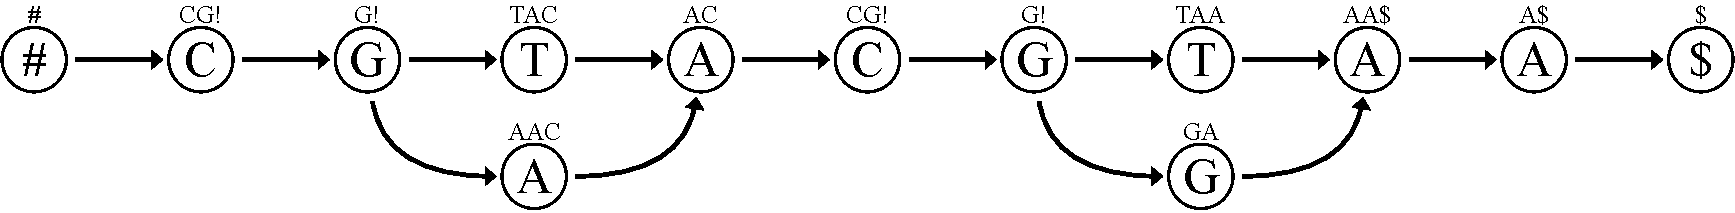
\includegraphics[width=\textwidth]{evo_gml_rev_det_but_not_prev_sort.pdf}
\caption[Reverse deterministic graph that is not prefix sorted]{Reverse deterministic graph that is not prefix sorted. Among others, the two nodes with label \textup{“C”} share the same prefix.} \label{fig:evo_gml_rev_det_but_not_prev_sort}
\end{figure}
If none of the nodes in the graph had more than one outgoing edge, then the graph 
would already be prefix sorted, as every prefix would end with the dollar sign 
and have this dollar sign in a different position than any of the other prefixes would. 
However, as the nodes in the graph we consider can actually have several outgoing edges, 
it is possible that they lead to nodes which have different labels. In this case, 
we write a special character such as the exclamation point at the character in the prefix, 
to note that this character can not be unambiguously determined. \\
The process of achieving a prefix sorted graph is therefore based on iterating through 
the nodes and reducing the amount of 
prefixes which end on exclamation points, as can be seen in algorithm~\ref{alg:workOnAutomatonPrefixes}. 
\begin{algorithm}
\caption[Prefix sort a graph]{Prefix sorting a graph by splitting nodes with prefixes that are not unambiguously sortable.}
\addtocontents{loa}{\vskip 15pt}
\label{alg:workOnAutomatonPrefixes}
\begin{algorithmic}[1]
\State $ \textrm{graph\_is\_not\_prefix\_sorted} \gets \texttt{true} $
\While{graph\_is\_not\_prefix\_sorted}
	\State $ \textrm{graph\_is\_not\_prefix\_sorted} \gets \texttt{false} $
	\ForAll {this\_node \textbf{in} graph}
		\State $ \textrm{this\_node.prefix} \gets \textrm{this\_node.label} $
	\EndFor
	\ForAll {this\_node \textbf{in} graph}
	\Comment {Check for all nodes...}
		\State $ \textrm{same\_as} \gets [ \, ] $
		\ForAll {that\_node \textbf{in} graph}
		\Comment {... if any node has the same prefix}
			\If {this\_node.prefix {\boldmath$ = $} that\_node.prefix}
				\State \textbf{append} $ [\textrm{that\_node}] $ \textbf{to} same\_as
			\EndIf
		\EndFor
		\If {\textbf{length of} $ \textrm{same\_as} > 1 $}
			\ForAll {node \textbf{in} same\_as}
			\Comment {Iterate over nodes with the same prefix}
				\State $ \textrm{first\_node\_label} \gets \textrm{next character to append to node.prefix} $
				\If {first\_node\_label cannot be found unambiguously}
					\State split the last node whose label was added to the prefix and which
						\State \phantom{first} has more than one successor
					\State $ \textrm{graph\_is\_not\_prefix\_sorted} \gets \texttt{true} $
				\Else
					\State \textbf{append} first\_node\_label \textbf{to} node.prefix
				\EndIf
			\EndFor
		\EndIf
	\EndFor
\EndWhile
\end{algorithmic}
\end{algorithm}
In line 18 of this algorithm, a node with more than one successor is split into several nodes. 
Such a node needs to exist there, as we reach this point in the algorithm due to a prefix 
not being unambiguously constructable, and the only way for this to happen is if a node has 
several successors with different prefixes. Therefore, we must be able to find a node with 
several successors for which splitting it enables us to build longer prefixes. \\
The exact approach for splitting a node $ N $ is to replace $ N $ by as many new nodes as $ N $ has 
outgoing edges. 
Every one of the nodes replacing $ N $ has exactly one outgoing edge, leading to 
one of the successors of $ N $. 
In this fashion, every successor of $ N $ obtains one of the nodes replacing $ N $ as predecessors. 
Every one of the new nodes also obtains incoming edges to all the nodes that are predecessors of $ N $. 
Finally, every one of the nodes replacing $ N $ is given the label of $ N $. 
The process of splitting a node is shown in figure~\ref{fig:evo_fig_node_splitting}.

% GACCTAATG|,5,C,8;,1,AG,5 - here we did a bit of work manually; this is about the splitting of the T node,
% but the position looks better after the splitting of the C node, so we copied some arrows manually in inkscape etc.
\begin{figure}[!htb]
\centering
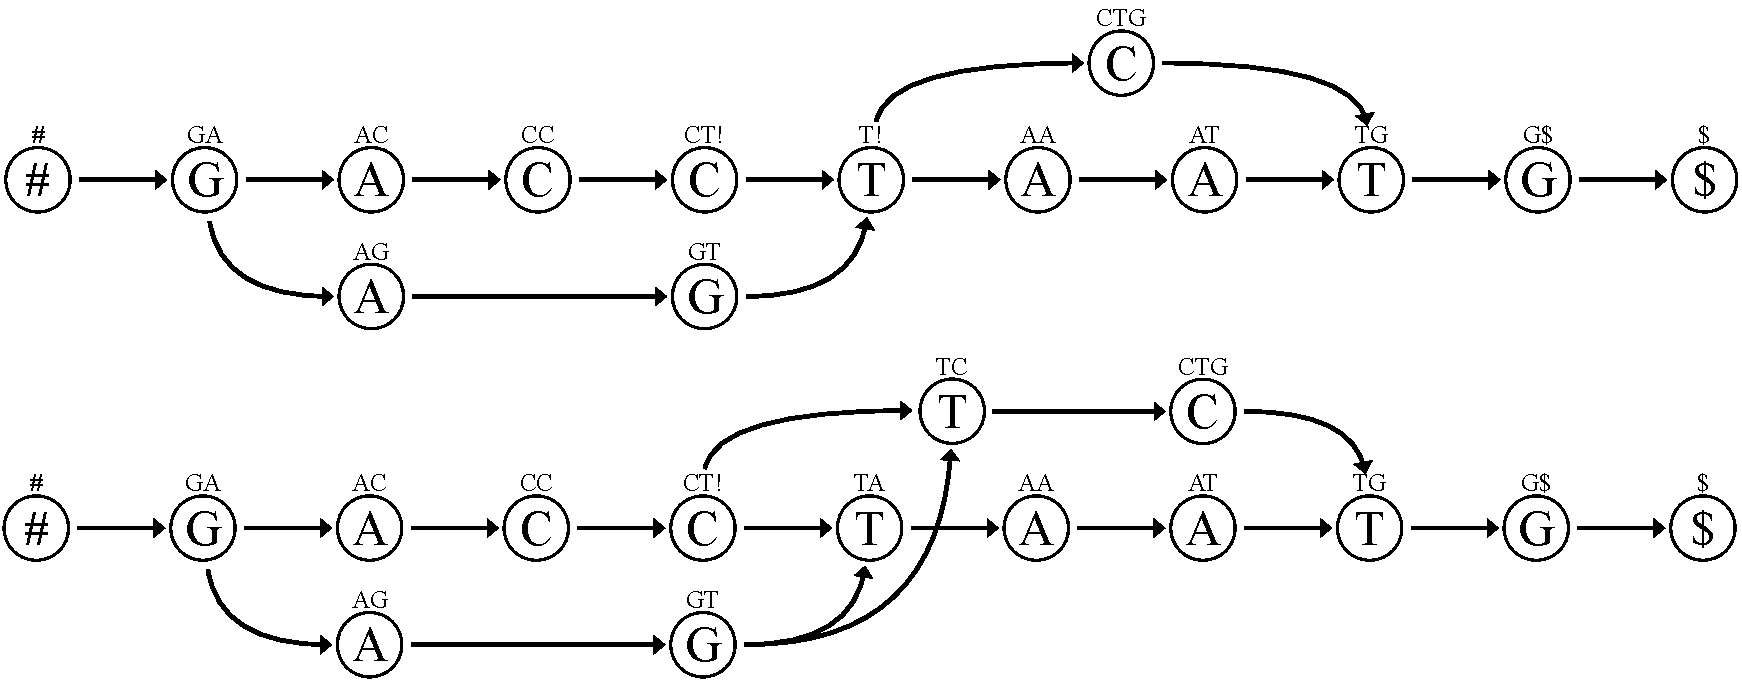
\includegraphics[width=\textwidth]{evo_fig_node_splitting.pdf}
\caption[Node splitting example]{Node splitting example. On the top, the graph is visualized before the splitting of the central node with label \textup{“T”} and prefix \textup{“T!”}. On the bottom, the same graph can be seen after node splitting occurred. The node has been replaced with one node with prefix \textup{“TC”} and one node with prefix \textup{“TA”}. Both nodes have all the incoming edges that the original node had.} \label{fig:evo_fig_node_splitting}
\end{figure}

It should be noted that we do not wish to remove all exclamation points entirely, 
as it is enough for a prefix to be so long as to be unambiguously sortable against all 
other prefixes of nodes in the graph. If a prefix is long enough to ensure this, then 
it is completely irrelevant whether it eventually ends in an exclamation point or in a dollar sign.

\section{Creating a Node Table}
%
% ~~~~~~~~~~~~~~~~~~~~~~~~~~~~~~~~~~~~~~~~~~~~~~~~~~~~~~~~~~~~~~~~~~~~~~~~~~~~~~~~~~~~~~~~~~~~~~~~~~~~~~~~~~~~~~~~~~~~~~~~~~~~~~~~~~~~
%                                                                                                       METHODS: Creating a Node Table
% ~~~~~~~~~~~~~~~~~~~~~~~~~~~~~~~~~~~~~~~~~~~~~~~~~~~~~~~~~~~~~~~~~~~~~~~~~~~~~~~~~~~~~~~~~~~~~~~~~~~~~~~~~~~~~~~~~~~~~~~~~~~~~~~~~~~~

Ultimately, we want to generate a flat XBW table from the prefix sorted graph, 
and explore methods for merging these flat XBW tables. 
However, in this section we first consider node tables, which share several characteristics 
with flat XBW tables. 
Node tables are easier to understand and to use as they are more closely related to the 
underlying graph, which means that the visualized graph can be used to understand their behaviour. 
The definition of a node table can be found in section~\ref{sec:node_table_definition}.

To create a node table when a prefix sorted graph such as the one in figure~\ref{fig:evo_fig_node_construct_prefixes} is given, 
% ACTAGTGAT|,5,T,8;,2,,4;,2,T,5
\begin{figure}[!htb]
\centering
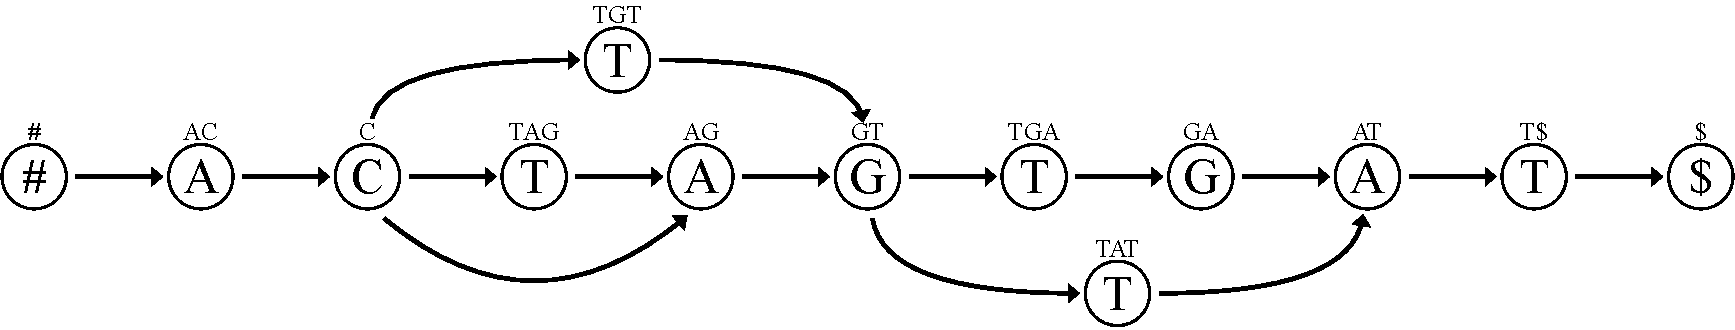
\includegraphics[width=\textwidth]{evo_fig_node_construct_prefixes.pdf}
\caption[Prefix sorted graph]{Prefix sorted graph, for which an XBW node table is supposed to be created.} \label{fig:evo_fig_node_construct_prefixes}
\end{figure}
we can first create 
an alphabetically sorted list of all prefixes of the nodes in the graph. 
Such as list is shown in table~\ref{table:node_construct_prefixes_1}.

\begin{table}[htb]
\centering
\caption[Alphabetically sorted prefix list]{Alphabetically sorted prefix list for the graph in figure~\ref{fig:evo_fig_node_construct_prefixes}.}
\begin{tabular}{ | c | c | c | c | c | c | c | c | c | c | c | c | c | c | }
\hline
\$ & AC & AG & AT & C & GA & GT & T\$ & TAG & TAT & TGA & TGT & \textbf{\#} & \textbf{Prefix} \\ \hline 
\end{tabular}
\label{table:node_construct_prefixes_1}
\end{table}

Having created such a list, we can then iterate over the list of prefixes. 
For each node $ v_i $ corresponding to prefix $ i $, 
we can add a cell for the value of the BWT and one for the value of the bit-vector $ M $ of $ v_i $. 
We store the labels of all nodes immediately 
preceding $ v_i $ in the BWT cell, 
and a string starting with a one followed by some amount of zeroes 
such that its overall length is equal to the outdegree of $ v_i $ in the $ M $ cell. \\
This gives us a table containing the prefixes, BWT and $ M $, such as table~\ref{table:node_construct_prefixes_2}.

\begin{table}[htb]
\centering
\caption[Node table with BWT, prefixes and $ M $]{Node table with BWT, prefixes and $ M $ for the graph in figure~\ref{fig:evo_fig_node_construct_prefixes}.}
\begin{tabular}{ | c | c | c | c | c | c | c | c | c | c | c | c | c | c | }
\hline
T & \textbf{\#} & T|C & G|T & A & T & A|T & A & C & G & G & C & \$ & \textbf{BWT} \\ \hline 
\$ & AC & AG & AT & C & GA & GT & T\$ & TAG & TAT & TGA & TGT & \textbf{\#} & \textbf{Prefix} \\ \hline 
1 & 1 & 1 & 1 & 100 & 1 & 10 & 1 & 1 & 1 & 1 & 1 & 1 & $\boldsymbol{M}$ \\ \hline 
\end{tabular}
\label{table:node_construct_prefixes_2}
\end{table}

We can finally also add a row for the bit-vector $ F $, with each cell containing 
a string starting with a one followed by as many zeroes as are necessary such that 
the length of the string is equal to the amount of entries of the corresponding BWT cell. 
This concludes the generation of the XBW node table for the given graph. 
An example outcome can be seen in table~\ref{table:node_construct_prefixes_3}.

\begin{table}[htb]
\centering
\caption[Complete node table]{Complete node table for the graph in figure~\ref{fig:evo_fig_node_construct_prefixes}.}
\begin{tabular}{ | c | c | c | c | c | c | c | c | c | c | c | c | c | c | }
\hline
T & \textbf{\#} & T|C & G|T & A & T & A|T & A & C & G & G & C & \$ & \textbf{BWT} \\ \hline 
\$ & AC & AG & AT & C & GA & GT & T\$ & TAG & TAT & TGA & TGT & \textbf{\#} & \textbf{Prefix} \\ \hline 
1 & 1 & 1 & 1 & 100 & 1 & 10 & 1 & 1 & 1 & 1 & 1 & 1 & $\boldsymbol{M}$ \\ \hline 
1 & 1 & 10 & 10 & 1 & 1 & 10 & 1 & 1 & 1 & 1 & 1 & 1 & $\boldsymbol{F}$ \\ \hline 
\end{tabular}
\label{table:node_construct_prefixes_3}
\end{table}

\section{Working on a Node Table}
%
% ~~~~~~~~~~~~~~~~~~~~~~~~~~~~~~~~~~~~~~~~~~~~~~~~~~~~~~~~~~~~~~~~~~~~~~~~~~~~~~~~~~~~~~~~~~~~~~~~~~~~~~~~~~~~~~~~~~~~~~~~~~~~~~~~~~~~
%                                                                                                     METHODS: Working on a Node Table
% ~~~~~~~~~~~~~~~~~~~~~~~~~~~~~~~~~~~~~~~~~~~~~~~~~~~~~~~~~~~~~~~~~~~~~~~~~~~~~~~~~~~~~~~~~~~~~~~~~~~~~~~~~~~~~~~~~~~~~~~~~~~~~~~~~~~~

Assuming that we have created a node table encoding a genomic graph, 
we can perform various operations on it. 
This includes going from one node in the table to its successors or predecessors, 
as well as reading out the prefix of a given node to a certain length.

\subsection{Navigating Through the Graph and Reading Out Labels}
\label{sec:gml_node_navigation}

To navigate through a graph represented by an XBW node table, 
we should be able to find the start and end nodes within the graph  
as well as being able to go from a node to a node connected to it through an edge.

To find the index $ i_s $ of the column representing the start node in a node table, 
we would usually search for all columns with a prefix starting with “$\#$”, 
as we know that the start node has a hash tag sign as its label. \\
As we assume there only to be one start node, there is only one such column in the node table. 
Its prefix therefore usually consists of just the letter “$\#$”, as there is no reason 
to build the prefix longer due to no other prefix starting with the same letter and an alphabetical 
ordering of the nodes by the prefixes being already guaranteed from just the first letter. 
However, a longer prefix would not be invalid, and therefore we would technically need to 
search for such a prefix starting with a hash tag sign. \\
Luckily, this entire search is unnecessary, as the single start node that is contained in the 
table can always be found in the same position. This position is the last, or right-most, column of the table. 
The reason why the column corresponding to the start node can always be found in this position is that 
the columns are alphabetically sorted by their prefixes, and the prefix of the start node starts with its label. 
The lexicographic value of this label is above the lexicographic value of all characters from the 
considered alphabet $ \Sigma $. \\
Equivalently, there is only one end node $ v_e $ in the graph, and the column with index $ i_e $ corresponding to it 
can always be found in the very first, or left-most, column of the node table. 
Therefore, we always have $ i_e \boldsymbol{=} 0 $.
The reason is here that the lexicographic value of the label “\$” is lower than that of all characters from the 
alphabet $ \Sigma $.

The problem of advancing from a node $ v $ to the preceding or succeeding nodes can 
be thought about in the context of reading out the labels of these preceding and succeeding nodes. 
To that end, we can assume that we are interested in a certain column $ i $ of the node table, 
which corresponds to a node $ v_i $ in the graph represented by the table. 
Reading out the label $ l ( v_i ) $ of that node itself can be achieved by reading out the prefix 
in column $ i $ of the table and taking the first character of this prefix.

To read out the label of a succeeding node, we actually have several possibilities. 
One way is to take the second character of the prefix of the current node, 
which corresponds to the first character of the prefix of each succeeding node, 
and therefore to their labels. This however only works if the prefix of $ v_i $ is 
given in the table with a length of more than one character, and if all succeeding nodes 
of $ v_i $ have the same label, as the prefix of $ v_i $ will otherwise have the 
error character “!” in the second position. \\
A similar approach can be used to read out the labels of the preceding nodes of $ v_i $. 
All these labels are different, as the graph has been made reverse deterministic, 
and they are stored in the BWT row of the node table. So if we find $ \textrm{BWT} ( i ) \boldsymbol{=} \textrm{A{\pipe}G} $, 
then we know that $ v_i $ has two preceding nodes with the labels A and G. 
This however only allows us to read out the labels of the immediately preceding nodes, 
while not enabling us to find the labels of nodes preceding the predecessors of $ v_i $.

A more robust approach for reading out labels of preceding and succeeding nodes 
is to use navigation functions to traverse the graph from $ v_i $ to the succeeding 
or preceding node that we are interested in, and to then read out the label of that 
node as first letter of its prefix. \\
To navigate the graph in the forward direction, that is, to find the immediate successors 
of a node $ v_i $, we can use the \texttt{nextNodes} function. Algorithm~\ref{alg:nextNodes} shows how this 
function works. 
\begin{algorithm}
\caption[Find succeeding nodes in a node table]{Given a column $ i $ in an XBW node table, find the indices of the columns corresponding to the succeeding nodes.}
\addtocontents{loa}{\vskip 15pt}
\label{alg:nextNodes}
\begin{algorithmic}[1]
\State $ \textrm{label} \gets \textrm{prefix} [ \, i \, ] [ \, 0 \, ] $
\State $ \textrm{jump\_over} \gets 0 $

\For {$ j $ \textbf{from} 0 \textbf{to} $ i $}
	\If {label {\boldmath$ = $} $ \textrm{prefix} [ \, j \, ] [ \, 0 \, ] $ }
		\State \textbf{increase} jump\_over
	\EndIf
\EndFor

\State $ \textrm{outdegree} \gets \textbf{length of} \, M [ \, i \, ] $
\State $ \textrm{nodes\_found} \gets [ \, ] $

\For {$ k $ \textbf{from} 0 \textbf{to length of} BWT}
	\If {$ \textrm{BWT} [ \, k \, ] $ \textbf{contains} label}
		\If {$ \textrm{jump\_over} > 0 $}
			\State \textbf{decrease} jump\_over
		\Else
			\State \textbf{decrease} outdegree
			\State \textbf{append} $ k $ \textbf{to} nodes\_found
			
			\If {$ \textrm{outdegree} < 1 $}
				\State \Return nodes\_found
			\EndIf
		\EndIf
	\EndIf
\EndFor
\end{algorithmic}
\end{algorithm}
The main idea behind this function is to add up all the lengths of the $ M $ values of 
the columns in the node table to the left of $ i $ which have the same label as $ v_i $ does. 
The resulting integer is stored in the variable jump\_over, as we intend to jump over that many 
nodes in the next step. 
We then iterate over the node table once more, this time reducing the amount of jump\_over by one for 
each column which contains the label of $ v_i $ in its BWT cell. 
When jump\_over reaches zero, we start adding the indices of the columns which we find to 
the output, until we have added as many indices as the outdegree of $ v_i $. \\
This approach works based on the fact that the left-most occurrence of a letter in the labels of the nodes corresponds 
to the left-most occurrence of this letter in the BWT, the second occurrence of a letter in the labels of the nodes 
corresponds to the second occurrence of this letter in the BWT, and so on.

A similar approach can be used to find the preceding nodes of $ v_i $, 
which has been implemented in the \texttt{prevNodes} function.

% ... - also write something about prevNodes! (maybe not quiiite so much though? who knows!)

\subsection{Constructing Prefixes}

If we are given the index of a column in the node table, corresponding to a node in the graph, 
then we can easily read out its prefix as the content of the prefix row in the given column. 
However, we might need to construct a longer prefix. 
Such a situation could arise if we were searching for a given text of length $ n $ within the 
graph, while the prefix we get from the table only has length $ m $ with $ m < n $. 
If the prefix agrees with the text for all the characters that are given, then we want to 
append more characters to the prefix until its length reaches $ n $ and a clear decision can 
be made on whether the prefix agrees with the text or not. \\
To construct such a longer prefix given a node table with short prefixes, we can use the 
idea of \textit{prefix doubling}. 
Hereby we do not append one character to the prefix at a time by iterating over the labels of succeeding nodes, 
but instead we append the entire prefixes of succeeding nodes. 
To actually find these succeeding nodes, we use the \texttt{nextNodes} function introduced in the previous section.

% ... TODO :: more? algorithm? At least some sort of figure illustrating this?
% (I guess a very very simple fake algorithm would actually do it here ^^)

% \subsection{Locating Strings in the Graph}
% 
% ... - add this section about how strings in the graph can be located!

\section{Merging Node Tables}
\label{sec:gml_merging_node_tables}
%
% ~~~~~~~~~~~~~~~~~~~~~~~~~~~~~~~~~~~~~~~~~~~~~~~~~~~~~~~~~~~~~~~~~~~~~~~~~~~~~~~~~~~~~~~~~~~~~~~~~~~~~~~~~~~~~~~~~~~~~~~~~~~~~~~~~~~~
%                                                                                                         METHODS: Merging Node Tables
% ~~~~~~~~~~~~~~~~~~~~~~~~~~~~~~~~~~~~~~~~~~~~~~~~~~~~~~~~~~~~~~~~~~~~~~~~~~~~~~~~~~~~~~~~~~~~~~~~~~~~~~~~~~~~~~~~~~~~~~~~~~~~~~~~~~~~

The main aim of the Graph Merging Library is to provide algorithms 
to merge and fuse flat XBW tables. 
However, working with flat XBW tables directly is rather cumbersome, 
and it can therefore help to first investigate the simpler case 
of merging two node tables.

\subsection{Basic Approach}

The general node table merging approach that we use 
in the function \texttt{merge\_BWTs\_advanced} 
is to add the columns of both tables which are supposed to be merged to a single table, 
to sort the columns in this new table by their prefixes, 
and to then expand prefixes until they all are unambiguous.

More exactly, we first add a row with the caption “origin” to both input tables, 
with all the cells of this row in the first table containing the character “0” and 
all the cells of the origin row in the second table containing the character “1”. 
We use these rows to later on keep track of where a node came from, 
such that we can perform operations on both input tables even while 
they are joined together within the emerging new table. \\
We then concatenate both tables to get one merged table containing 
nodes from both input tables. 
We also replace the label of the end node of the first table with $\$_0$ and 
the label of the start node of the second table with $\#_0$, to easier keep track 
of which start and end node is really contained in the final graph 
and which one is only used while merging and will be discarded later on. \\
We can then sort all columns alphabetically according to their prefixes. 
If this does not lead to ambiguities due to columns with different origins 
sharing the same prefixes, then we are lucky. However, if this occurs, 
then we have to continue constructing the prefixes of these ambiguous nodes, 
until all the ambiguities have been resolved. \\
Finally, we can take out the $\$_0$ and $\#_0$ nodes which are no longer needed 
and drop the origin row to convert the table we were constructing into 
a fully merged XBW node table.

% ... - illustrate this more, using figures and tables and things! =)

% Algorithm for Merging Node Tables (function GML.merge_BWTs_advanced()):
%
% find last letter of DH_1 and first letter of DH_2
% > yepp, this is truly the label of the node BEFORE $ / the label of the node AFTER #,
%   so this assumes that there is only one edge into $ and only one edge out of #!
%
% add origin to H_1 and H_2
% concatenate H_1 and H_2 as H_12
% replace $ having origin 0 with $#firstLetterH_2 within prefixes
% and more

\subsection{Aftersort Array}

While working on the emerging XBW node table, we often have to construct longer prefixes for nodes 
with ambiguous prefixes. Do do so, we navigate through the graph and append labels of the nodes we encounter. 
However, this navigation through the graph is made more difficult by the fact that the ordering 
of the nodes of the first input table can be changed within the merged table. 
The reason for this is that their prefixes, which within the first input table ended at the 
end node $ v_e $ of the first graph, can now spill over into the second graph, 
thereby giving different relative orderings. 
This concept is illustrated in figure~\ref{fig:evo_fig_node_merge_aftersort} and table~\ref{table:node_merge_aftersort}. \\
% GAAT|,1,CT,3 and CAA|,1,,3
\begin{table}[htb]
\centering
\caption[Node tables showing purpose of aftersort array]{Node tables showing the purpose of the aftersort array. The upper two node tables are the inputs for the XBW node merging, while the bottom table is the outcome. The highlighted columns correspond to the highlighted nodes in figure~\ref{fig:evo_fig_node_merge_aftersort}.}

{
% reduce whitespace in this table (default might be 6pt)
\renewcommand{\tabcolsep}{4pt}
\begin{tabular}{ | c | c | c | c | c | c | c | c | c | }
\hline
T & G & A|T & G & $\#$ &\cellcolor{green_bg}\color{green_fx}A &\cellcolor{purple_bg}\color{purple_fx}C & \$ & \textbf{BWT} \\ \hline 
\$ & AA & AT & C & G &\cellcolor{green_bg}\color{green_fx}T\$$\#$C &\cellcolor{purple_bg}\color{purple_fx}TA & $\#$ & \textbf{Prefix} \\ \hline 
1 & 1 & 1 & 1 & 10 &\cellcolor{green_bg}\color{green_fx}1 &\cellcolor{purple_bg}\color{purple_fx}1 & 1 & $\boldsymbol{M}$ \\ \hline 
1 & 1 & 10 & 1 & 1 &\cellcolor{green_bg}\color{green_fx}1 &\cellcolor{purple_bg}\color{purple_fx}1 & 1 & $\boldsymbol{F}$ \\ \hline 
\end{tabular}
\quad
\begin{tabular}{ | c | c | c | c | c | c | }
\hline
A & A|C & C & $\#$ & \$ & \textbf{BWT} \\ \hline 
\$ & A\$ & AA & C & $\#$ & \textbf{Prefix} \\ \hline 
1 & 1 & 1 & 10 & 1 & $\boldsymbol{M}$ \\ \hline 
1 & 10 & 1 & 1 & 1 & $\boldsymbol{F}$ \\ \hline 
\end{tabular}
}

\vspace{0.5cm}

\begin{tabular}{ | c | c | c | c | c | c | c | c | c | c | c | c | }
\hline
A & A|C & C & G & A|T & T & G & $\#$ &\cellcolor{purple_bg}\color{purple_fx}C &\cellcolor{green_bg}\color{green_fx}A & \$ & \textbf{BWT} \\ \hline 
\$ & A\$ & AA\$ & AAT & AT & CA & CT & G &\cellcolor{purple_bg}\color{purple_fx}TA &\cellcolor{green_bg}\color{green_fx}TC & $\#$ & \textbf{Prefix} \\ \hline 
1 & 1 & 1 & 1 & 1 & 10 & 1 & 10 &\cellcolor{purple_bg}\color{purple_fx}1 &\cellcolor{green_bg}\color{green_fx}1 & 1 & $\boldsymbol{M}$ \\ \hline 
1 & 10 & 1 & 1 & 10 & 1 & 1 & 1 &\cellcolor{purple_bg}\color{purple_fx}1 &\cellcolor{green_bg}\color{green_fx}1 & 1 & $\boldsymbol{F}$ \\ \hline 
\end{tabular}

\label{table:node_merge_aftersort}
\end{table}
% GAAT|,1,CT,3 and CAA|,1,,3
\begin{figure}[!htb]
\centering
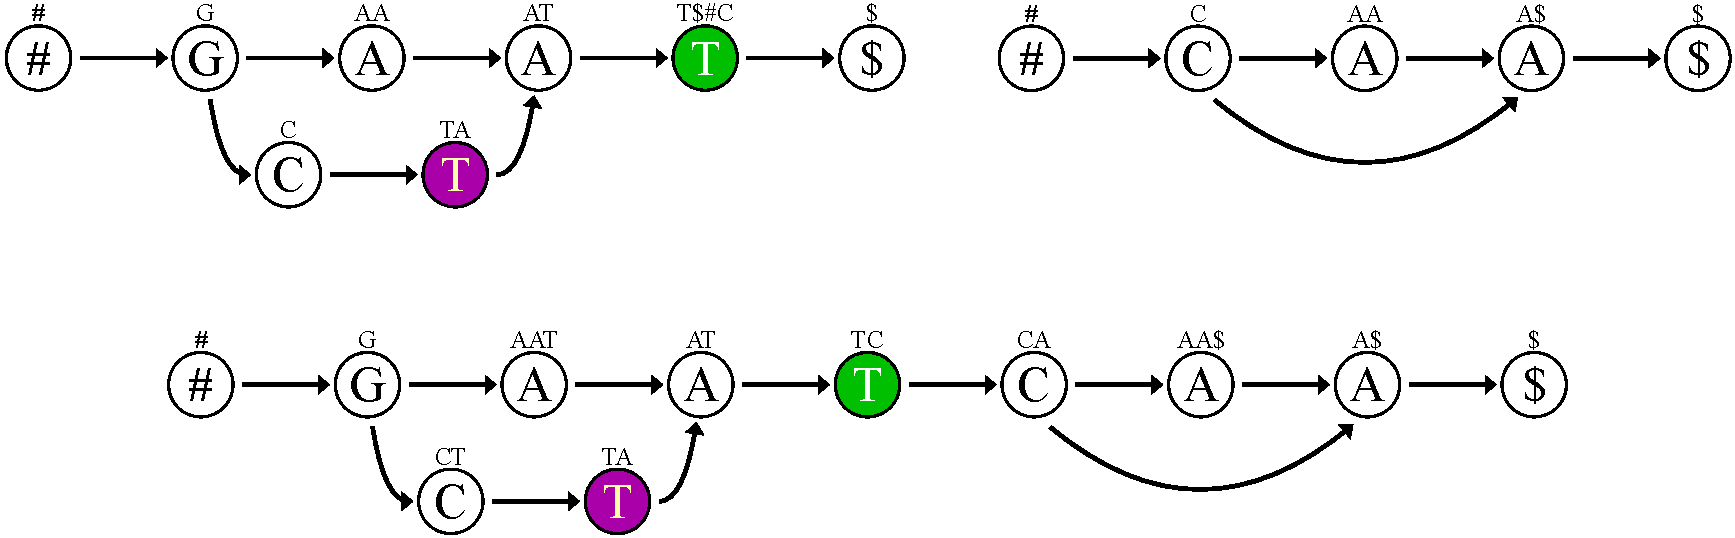
\includegraphics[width=\textwidth]{evo_fig_node_merge_aftersort.pdf}
\caption[Graphs showing purpose of aftersort array]{Graphs showing the purpose of the aftersort array. The upper two graphs correspond to the inputs for the XBW node merging, while the bottom graph corresponds to the outcome. The highlighted nodes correspond to the highlighted columns in table~\ref{table:node_merge_aftersort}.} \label{fig:evo_fig_node_merge_aftersort}
\end{figure}
% TODO :: make sure that these two (the table and the figure) actually end up on the same page, and are not split over several pages
We can see that in the input table at the top, the green node with prefix T\$$\#$C is sorted 
before the purple node with prefix TA, 
as the dollar sign is lexicographically smaller 
than all other considered characters. 
When considering just the first input table on its own, the prefix of the green node would actually be T\$, 
as we only appended $\#$C to that prefix is to show 
how the prefix will look like when a spillover into the second input graph occurs, in which labels from the 
second input graph are appended to prefixes in the first graph. 
However, in the merged table at the bottom, the green node with prefix TC is sorted after the purple node with prefix TA, 
as “C” is lexicographically bigger than “A”. \\
Therefore, when we are working with the merged table, we cannot simply append the columns from the two input 
tables in the exact order in which they are within the input tables, but we need to change the order slightly 
to account for the fact that such spillovers from the first into the second input can happen. 
This itself is not a particularly challenging problem, as we can just account for this different sorting 
behaviour when initially constructing the merged table. \\
However, doing so results in a merged table which is internally inconsistent as long as we still 
see it as merged form of two individual tables, using an origin row to keep track of the partial table 
we are working in. 
To counteract this problem, we use a structure which we refer to as an \textit{aftersort array}, 
which allows us to account for sorting problems after the start of merging the two tables. 
It provides a mapping from the locations within the first input table that we expect 
to the actual locations in the merged table, which can slightly differ from it. 
In particular, we use such an array with the name bwt\_aftersort in 
the functions \texttt{nextNodes} and \texttt{prevNodes} to this end. \\
It is never necessary to apply an aftersort array when considering the second input, 
as no spillovers out of that table can occur when building prefixes, as we build 
prefixes by advancing to succeeding nodes, and no new node is succeeding the end node 
of the second input which actually becomes the end node of the merged table.

\section{Creating a Flat Table}
%
% ~~~~~~~~~~~~~~~~~~~~~~~~~~~~~~~~~~~~~~~~~~~~~~~~~~~~~~~~~~~~~~~~~~~~~~~~~~~~~~~~~~~~~~~~~~~~~~~~~~~~~~~~~~~~~~~~~~~~~~~~~~~~~~~~~~~~
%                                                                                                       METHODS: Creating a Flat Table
% ~~~~~~~~~~~~~~~~~~~~~~~~~~~~~~~~~~~~~~~~~~~~~~~~~~~~~~~~~~~~~~~~~~~~~~~~~~~~~~~~~~~~~~~~~~~~~~~~~~~~~~~~~~~~~~~~~~~~~~~~~~~~~~~~~~~~

We now wish to create a flat XBW table based on a node table. 
% TODO :: later on also create a flat XBW table directly, without the node table in between?
For the general definition of such a flat table, see section~\ref{sec:flat_table_definition}.

The process of converting an XBW node table into a flat table is illustrated in tables~\ref{table:evo_node_to_flat_node} 
and \ref{table:evo_node_to_flat_flat}, which respectively show the a node table and a flat table representing the same graph. \\
% GATAATG|,3,C,6;,1,AG,3
{
% reduce whitespace in this table (default is might be 6pt)
\renewcommand{\tabcolsep}{5pt}
\begin{table}[htb]
\centering
\caption[XBW node table before conversion to flat table]{XBW node table before conversion to flat table. 
Table~\ref{table:evo_node_to_flat_flat} shows the corresponding flat table.}
\begin{tabular}{ | c | c | c | c | c | c | c | c | c | c | c | c | c | c | c | }
\hline
G & T & G & G & G & A & T & T & $\#$ & A & A|G & A|G & A|C & \$ & \textbf{BWT} \\ \hline 
\$ & AA & AG & ATA & ATC & ATG & C & G\$ & GA & GT & TA & TC & TG & $\#$ & \textbf{Prefix} \\ \hline 
1 & 1 & 1 & 1 & 1 & 1 & 1 & 1 & 100 & 10 & 1 & 1 & 1 & 1 & $\boldsymbol{M}$ \\ \hline 
1 & 1 & 1 & 1 & 1 & 1 & 1 & 1 & 1 & 1 & 10 & 10 & 10 & 1 & $\boldsymbol{F}$ \\ \hline 
\end{tabular}
\label{table:evo_node_to_flat_node}
\end{table}
}
\begin{table}[htb]
\centering
\caption[Flat XBW table after conversion from node table]{Flat XBW table after conversion from node table. 
Table~\ref{table:evo_node_to_flat_node} shows the corresponding node table.}
\begin{tabular}{ | c | c | c | c | c | c | c | c | c | c | c | c | c | c | c | c | c | c | }
\hline
G & T & G & G & G & A & T & T & $\#$ & A & A & G & A & G & A & C & \$ & \textbf{BWT} \\ \hline 
\$ & A & A & A & A & A & C & G & G & G & G & G & G & T & T & T & $\#$ & \textbf{FC} \\ \hline 
1 & 1 & 1 & 1 & 1 & 1 & 1 & 1 & 1 & 0 & 0 & 1 & 0 & 1 & 1 & 1 & 1 & $\boldsymbol{M}$ \\ \hline 
1 & 1 & 1 & 1 & 1 & 1 & 1 & 1 & 1 & 1 & 1 & 0 & 1 & 0 & 1 & 0 & 1 & $\boldsymbol{F}$ \\ \hline
\end{tabular}
\label{table:evo_node_to_flat_flat}
\end{table}
% TODO :: make certain that the previous two figures end up on the same page!
For the BWT, $ M $ and $ F $ rows, the process of achieving this conversion is exactly the same. 
We join all the cells together to achieve one string containing the entire 
row, and then split this row in between every character. 
If there were pipe characters in between some of the characters, such as 
for visualization purposes within the BWT cells, then we omit them in this process. \\
The process for the prefixes is a little bit different, as the flat XBW table does 
not contain the whole prefixes due to their immense size. 
The flat XBW table can however be thought of as containing FC, the first column data (where 
the first column refers to the first column of the alphabetically sorted cyclic rotations, 
not to the first column of this table.) 
As the FC field corresponds to the label of the node, and as the prefixes in the node table 
begin with the labels of their respective nodes, the two rows are intimately linked 
and the FC row can be constructed from the prefixes in the node table. 
For the construction of the FC row, it is also necessary to consider the amount of 
outgoing edges of a node, which is encoded in $ M $. 
In total, to generate the FC row in the flat table based on the prefix and $ M $ rows in the 
node table, we start with an empty string for FC and iterate through the prefixes in the node table. 
For each prefix, we read out the first character of that prefix. 
We then add this first character as often to FC, as the contents of the $ M $ cell 
in the corresponding column are long. So if the value of $ M $ is 100, 
then the first character of that prefix needs to be added three times to FC. \\
Having constructed the BWT, FC, $ M $ and $ F $ rows from the original node table, 
we have now created a flat XBW table which represents the same graph that was represented 
by the original table.

\section{Working on a Flat Table}
%
% ~~~~~~~~~~~~~~~~~~~~~~~~~~~~~~~~~~~~~~~~~~~~~~~~~~~~~~~~~~~~~~~~~~~~~~~~~~~~~~~~~~~~~~~~~~~~~~~~~~~~~~~~~~~~~~~~~~~~~~~~~~~~~~~~~~~~
%                                                                                                     METHODS: Working on a Flat Table
% ~~~~~~~~~~~~~~~~~~~~~~~~~~~~~~~~~~~~~~~~~~~~~~~~~~~~~~~~~~~~~~~~~~~~~~~~~~~~~~~~~~~~~~~~~~~~~~~~~~~~~~~~~~~~~~~~~~~~~~~~~~~~~~~~~~~~

The next section is about the merging of several flat XBW tables. 
Before considering this rather challenging problem, 
it is helpful to first investigate how work within such flat tables can be performed in general. 
In particular, we here look at how 
the functions \texttt{LF} and $ \Psi $ can be used to find the predecessors and successors 
of nodes, respectively.

\subsection{Graph Navigation}

As with the navigation through XBW node tables described in section~\ref{sec:gml_node_navigation}, 
the navigation through a graph represented by a flat XBW table relies on 
being able to find special nodes within the graph  
as well as being able to advance from one node to another one. 
In particular, we should to be able to find the start node and the end node in the flat table, 
and given a node $ v $, we should be able to find the preceding and the succeeding nodes of $ v $.

% find start node
To find the cells corresponding to the start node $ v_s $, we can again look at the end of the table, 
just as when finding the start node in a node table. 
However, in this case it is not enough to look at the last column, as some other cells could belong 
to the start node too. In particular, as the start node can have several outgoing edges, 
there could be several cells in the FC and $ M $ rows corresponding to the start node. 
Therefore, using FC-indexing or BWT-indexing complicates finding the start node slightly, 
while finding this node with absolute indexing is as simple as for node tables. \\
In absolute indexing, the index $ i_s $ of the start node is the highest index of all nodes. 
It can be found as $ i_s \boldsymbol{=} \textrm{rank}_1 ( M, l ) \boldsymbol{=} \textrm{rank}_1 ( F, l ) $ where we 
define $ l $ as the index of the last column in the table, 
which is equal to one less than the amount of columns in the table. \\
% find end node
Finding the cells corresponding to the end node $ v_e $ is even simpler, as its label “\$” is 
lexicographically smaller than all other labels and it is therefore sorted to the very front. 
This means that the absolute index of the end node in a flat table is $ i_e \boldsymbol{=} 0 $. 
As there can be no nodes preceding this one in the table, the index is also 0 when using 
FC-indexing or BWT-indexing.

% find preceding nodes
To find the preceding nodes of a given node, 
we can use the function \texttt{LF}. It performs last-to-first mapping to 
map the last column in the matrix of sorted cyclic rotations, which is the BWT, 
to the first column, which is the FC row. 
How this function operates can be seen in algorithm~\ref{alg:lf}. 
\begin{algorithm}
\caption[\texttt{LF} function for flat table navigation]{\texttt{LF} function for flat table navigation which takes in an absolutely indexed range $ [ sp, ep ] $ and a character $ c $. It gives out an absolutely indexed range corresponding to nodes with label $ c $ preceding the ones that were put in.}
\addtocontents{loa}{\vskip 15pt}
\label{alg:lf}
\begin{algorithmic}[1]

\State $ sp \gets \textrm{select}(1, F, sp) $
\Comment{If do\_select: absolute indexing to BWT-indexing}
\State $ ep \gets \textrm{select}(1, F, ep + 1) - 1 $

\State \phantom{nl}

\State $ sp \gets C [ c ] + \textrm{rank}(c, \textrm{BWT}, sp - 1) + 1 $
\Comment{Perform last-to-first mapping}
\State $ ep \gets C [ c ] + \textrm{rank}(c, \textrm{BWT}, ep) $

\State \phantom{nl}

\If {ep < sp}
\Comment{Return empty range if nothing is found}
	\State \Return $ [ \, ] $
\EndIf

\State \phantom{nl}

\State $ sp \gets \textrm{rank}(1, M, sp) $
\Comment{If do\_rank: FC-indexing to absolute indexing}
\State $ ep \gets \textrm{rank}(1, M, ep) $

\State \phantom{nl}

\State \Return $ [ sp, ep ] $

\end{algorithmic}
\end{algorithm}
Its general approach is to take in a range $ [ sp, ep ] $ of absolute indices of 
nodes $ v_{sp}, ..., v_{ep} $ and a character $ c $, 
and return a range of absolute indices corresponding to the nodes 
preceding the ones that were given as input which have character $ c $ as label. 
Both ranges can represent one or several nodes. \\
The \texttt{LF} function is more general than a function designed for just finding the 
preceding nodes of a given node. The ability of taking in more than one node through 
the input range combined with the ability to actively search for specific preceding 
nodes through the character $ c $ means that it can actually be used when searching 
for texts within the graph. 
However, it can of course also be used to just find the preceding nodes of a given node $ v_i $, 
by calling it once for each BWT entry corresponding to $ v_i $. \\
E.g. if two BWT entries correspond to $ v_i $, then the function needs to be called twice, 
with the character $ c $ set to a different one of these BWT entries each time. 
The resulting ranges will describe one node each time, 
giving us a total of two preceding nodes for the input node. \\
We here made the select operations in the beginning and the rank operations in 
the end optional by introducing the parameters do\_select and do\_rank, 
so that the caller can set them to \texttt{false} after 
deciding to use different indexing methods if that is more convenient.

% find succeeding nodes
Similar to the \texttt{LF} function for preceding nodes, there is also a second special function we can use 
to find the succeeding nodes of a given node. 
This function is called $ \Psi $ and its approach is shown in algorithm~\ref{alg:psi}. 
\begin{algorithm}
\caption[$ \Psi $ function for flat table navigation]{$ \Psi $ function for flat table navigation which takes in an absolute index $ i $ and an edge number $ j $. It gives out the absolute index of the $ j $th node succeeding the node with index $ i $.}
\addtocontents{loa}{\vskip 15pt}
\label{alg:psi}
\begin{algorithmic}[1]

\State $ i \gets \textrm{select}(1, M, i) $
\Comment{If do\_select: absolute indexing to FC-indexing}

\State \phantom{nl}

\State $ i \gets i + j $
\State $ c \gets \textrm{FC} [ i ] $
\State $ i \gets \textrm{select}(c, \textrm{BWT}, i - C [ c ]) $
\Comment{Get the next node}

\State \phantom{nl}

\State $ i \gets \textrm{rank}(1, F, i) $
\Comment{If do\_rank: BWT-indexing to absolute indexing}

\State \phantom{nl}

\State \Return $ i $

\end{algorithmic}
\end{algorithm}
It works slightly different than \texttt{LF}, 
in that it does not work on a range of nodes, but instead focuses on a single node only. 
Similarly to \texttt{LF}, we need to call $ \Psi $ several times to find all nodes succeeding a given one. 
This functionality is provided through a second parameter which $ \Psi $ takes 
in addition to the index of the node we are examining. 
The second parameter determines which edge we take out of that node, 
and the index of the single node which we reach upon using that edge is returned. \\
More formally, when $ i $ is the absolute index of a node $ v_i $ in the flat XBW table, 
and $ j $ is an integer, then $ \Psi (i, j) $ returns the absolute index of the $ j $th node 
succeeding the node $ v_i $. So if the node $ v_i $ has two outgoing edges, 
then $ \Psi (i, 0) $ returns the absolute index of the node reached when following 
the first of these edges, while $ \Psi (i, 1) $ returns the absolute index of the node reached when 
taking the second outgoing edge. \\
The $ \Psi $ function described here differs slightly from the one proposed by \citet{Siren2014}. 
One of the differences is that we convert from absolute indexing to FC-indexing first, 
and then get the character $ c $, as we directly take $ c $ from the FC row instead 
of using another structure which corresponds to the FC row without entries for which $ M $ is zero. 
The second difference is that we use $ j \boldsymbol{=} 0 $ to indicate the first outgoing edge, 
while their function starts with $ j \boldsymbol{=} 1 $. 
Finally, in our version we actually made the select operation in the beginning and the rank operation in 
the end optional by introducing the parameters do\_select and do\_rank, 
just as we did with the \texttt{LF} function. 
This in particular allows the caller to combine the parameters $ i $ and $ j $ into one value 
when calling with FC-indexing by setting do\_select to \texttt{false}, 
therefore preventing unnecessary indexing method conversions.

% TODO :: maybe add a table or figure showing an example run of LF and Psi?

\subsection{Constructing Prefixes}
\label{sec:gml_flat_construct_prefixes}

Prefixes can be constructed using the $ \Psi $ function to advance from a node to the next ones, 
while keeping track of the labels of these nodes. \\
That is, to construct the prefix of a node $ v $, we can read out the label $ l ( v ) $ as 
first character of the prefix. 
We can then advance through all nodes $ u_j $ succeeding $ v $ by using the $ \Psi $ function once 
for each outgoing edge. 
If all these nodes $ u_j $ have the same label, so if $ l ( u_j ) \boldsymbol{=} l ( u_k ) $ for 
all $ j $ and $ k $ for which $ u_j $ and $ u_k $ are defined, then we can append this label 
to the prefix we are building. 
Otherwise, we have to append an error character such as “!” to indicate that this position in the 
prefix cannot be filled unambiguously and stop the prefix generation. 
We also have to stop building up the prefix when we add the special “\$” character to it, 
as we would otherwise just continue building it from the start. 
We can continue onwards with this process until we have generated a prefix of the desired length 
by repeatedly using $ \Psi $ again to find all succeeding nodes 
of all current nodes $ u_j $, and again adding the shared label of all of them if it is unambiguous. \\
This process is implemented in the function \texttt{\_publishPrefix} of the XBW environment in GML. 
Its general approach is outlined in algorithm~\ref{alg:_publishPrefix}. 
\begin{algorithm}
\caption[Generate prefix of a node in a flat table]{Generate the prefix of a node with FC-index $ i $ in a flat XBW table up to a given length. The optional parameter use\_all\_out\_edges can be set to \texttt{true} such that all outgoing edges of the specified node are used. Otherwise, only the specific edge addressed by $ i $ is followed out of the first considered node.}
\addtocontents{loa}{\vskip 15pt}
\label{alg:_publishPrefix}
\begin{algorithmic}[1]

\State $ \textrm{pref} \gets \texttt{\textquotesingle}\texttt{\textquotesingle} $
\State $ \textrm{i\_arr} \gets [ i ] $

\For {$ i $ \textbf{from} 0 \textbf{to} length}

	\If {$ (i > 0) $ \textbf{or} use\_all\_out\_edges}
		\State $ \textrm{len} \gets \textrm{\textbf{length of} i\_arr} $
		\For {$ j $ \textbf{from} 0 \textbf{to} len}
			\If {i > 0}
			\Comment {Convert from absolute}
				\State $ \textrm{i\_arr}[ j ] \gets \textrm{select}(1, M, \textrm{i\_arr}[ j ]) $
				\Comment {indexing to FC-indexing}
			\Else
				\State \textbf{decrease} i\_arr$[ j ]$ \textbf{while} $ M [ \textrm{i\_arr$[ j ]$} ] \boldsymbol{=} 0 $
			\EndIf

			\For {$ k $ \textbf{from} 1 \textbf{until} $ M [ \textrm{pref\_cur\_is$[ j ] + k$} ] \neq 0 $}
				\State \textbf{append} i\_arr$[ j ] + k $ \textbf{to} i\_arr
			\EndFor
		\EndFor
	\EndIf

	\For {$ j $ \textbf{from} 0 \textbf{to length of} i\_arr}
	\Comment{Follow a specific outgoing edge}
		\State $ \textrm{i\_arr}[ j ] \gets \Psi(\textrm{i\_arr}[ j ], 0, \texttt{false}, \texttt{false}) $
		\Comment{in FC-indexing and get the}
	\EndFor
	\Comment{answer in BWT-indexing}

	\State $ \textrm{char\_to\_add\_now} \gets \textrm{BWT}[ \textrm{i\_arr$[ 0 ]$} ] $
	\State $ \textrm{not\_all\_chars\_are\_the\_same} \gets \texttt{false} $

	\For {$ j $ \textbf{from} 0 \textbf{to length of} i\_arr}
		\If {$ \textrm{char\_to\_add\_now} \neq \textrm{BWT}[ \textrm{i\_arr$[ j ] $} ] $}
			\State $ \textrm{not\_all\_chars\_are\_the\_same} \gets \texttt{true} $
		\EndIf
	\EndFor

	\If {not\_all\_chars\_are\_the\_same}

		\State $ \textrm{pref} \gets \textrm{pref} + \textrm{\texttt{\textquotesingle}!\texttt{\textquotesingle}} $
		\Comment{Add error char to the prefix}

		\State \textbf{break}

	\Else

		\State $ \textrm{pref} \gets \textrm{pref} + \textrm{char\_to\_add\_now} $

		\If {($ \textrm{\textbf{length of} pref} > 1 $) \textbf{and} ($ \textrm{char\_to\_add\_now} \boldsymbol{=} \textrm{\texttt{\textquotesingle}$\$_0$\texttt{\textquotesingle}} $)}
		\Comment{Spillover}

			\State $ i \gets (\textrm{\textbf{length of} FC row in nextXBW}) - 1 $
			\Comment{Find $\#_0$ node in next XBW}

			\State \Return pref + nextXBW.\texttt{\_publishPrefix}$( i )$
		\EndIf
	\EndIf

	\If {(char\_to\_add\_now {\boldmath$ = $} \texttt{\textquotesingle}\$\texttt{\textquotesingle}) \textbf{or} (char\_to\_add\_now {\boldmath$ = $} \texttt{\textquotesingle}$\$_0$\texttt{\textquotesingle})}
		\State \textbf{break}
	\EndIf

	\For {$ j $ \textbf{from} 0 \textbf{to length of} i\_arr}
	\Comment{Convert from BWT-indexing}
		\State $ \textrm{i\_arr}[ j ] \gets \textrm{rank}(1, F, \textrm{i\_arr}[ j ]) $
		\Comment{to absolute indexing}
	\EndFor
\EndFor

\State \Return pref

\end{algorithmic}
\end{algorithm}
As the input to the function is given with the FC-indexing method, a particular edge can be specified 
via which the first node is supposed to exited. This can be helpful for specific visualization purposes. 
However, usually this is not the intended behaviour, which is why we introduced the parameter 
use\_all\_out\_edges which defaults to \texttt{true}. 
When it is left at its default value, all outgoing edges from the input node are considered, 
just as they should be to generate the real prefix of the node. Therefore, the parameter can usually be ignored. 
Only when it is explicitly set to \texttt{false} does the edge given by the input matter, 
as the other outgoing edges of the input node are then not visited while generating the prefix. 
The differences between the two possible choices for this parameter 
are shown in figure~\ref{fig:evo_fig_use_all_out_edges_or_not}. \\
% GACGT|,2,T,4;,3,,5 and ACCT|,1,,4;,1,,3
\begin{figure}[!htb]
\centering
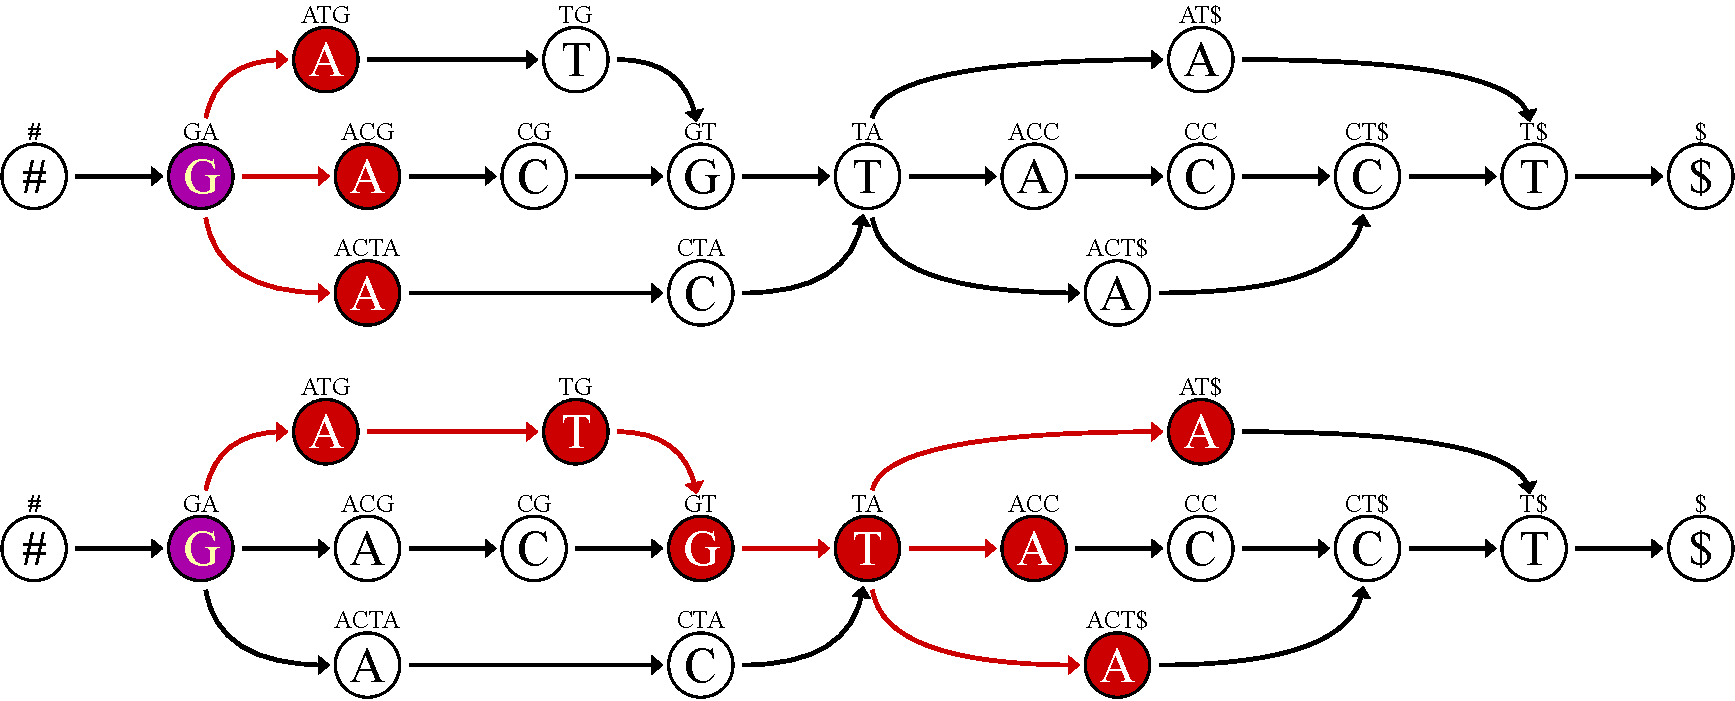
\includegraphics[width=\textwidth]{evo_fig_use_all_out_edges_or_not.pdf}
\caption[Prefix generation in a flat table with use\_all\_out\_edges]{Prefix generation in a flat table with \textup{use\_all\_out\_edges}. We here called \textup{\texttt{\_publishPrefix}} for the node with prefix \textup{“GA”} highlighted in purple. At the top, we set \textup{use\_all\_out\_edges} to its default value \textup{\texttt{true}}, and therefore the prefix \textup{“GA!”} is returned. The prefix becomes ambiguous with the possibilities of constructing it as \textup{“GAT”} or \textup{“GAC”}. At the bottom, we set \textup{use\_all\_out\_edges} to \textup{\texttt{false}} and choose exactly one edge leading out of the purple node. This leads to the prefix \textup{“GATGTA!”} being generated.} \label{fig:evo_fig_use_all_out_edges_or_not}
\end{figure}
In addition to performing the aforementioned calculations to generate the prefix of a given node, 
this function can also return a recommended \textit{split node} through the optional parameter give\_the\_split\_node. 
The computations necessary for this have not been included in algorithm~\ref{alg:_publishPrefix} to simplify 
the understanding of it, but they basically consist of an array of visited paths which keeps track 
of the potential split nodes, and an evaluation at the very end of the function which determines 
which one of these to return by choosing a node actually on a path leading to a prefix ambiguity. 
We here define a split node as a node which can be split into several nodes, thereby ideally enabling us 
to continue building longer prefixes. 
An example for such a node can be seen in figure~\ref{fig:evo_split_node}. 
% GTCTTAACT|,3,AG,5
\begin{figure}[!htb]
\centering
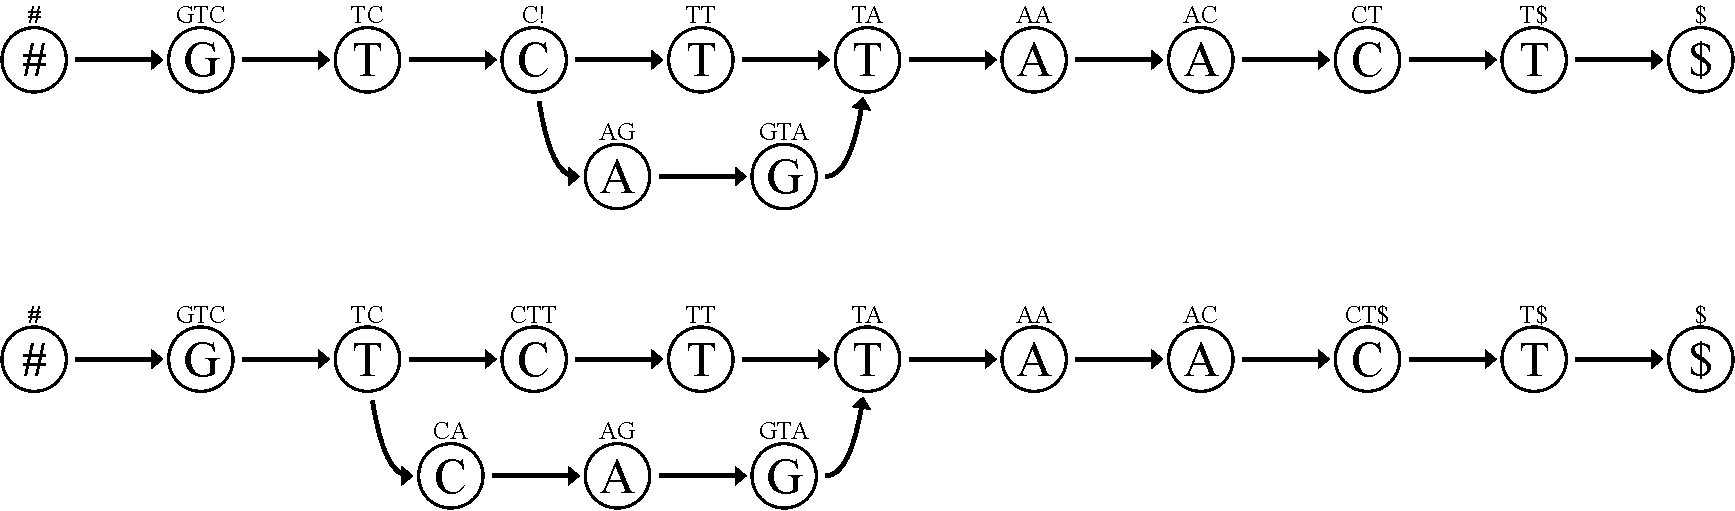
\includegraphics[width=\textwidth]{evo_split_node.pdf}
\caption[Graph with split node before and after splitting]{Graph with split node having prefix \textup{“C!”} before splitting (top) and the same graph after splitting the node (bottom).} \label{fig:evo_split_node}
\end{figure}
It can be seen that splitting the node with label “C!” in the figure did not change the 
genomic strings generated as paths through the whole graph from start node to end node, 
which is a general requirement we have for splitting nodes. 
The splitting helped in enabling us to build longer prefixes as one node with 
two outgoing edges to nodes with different labels was replaced by two nodes 
with only one outgoing edge each, so that each one of the new nodes can 
have a longer prefix. \\
For the general concept of splitting nodes to 
enable the building of longer prefixes, see section~\ref{sec:prefix_sorting}. \\
In figure~\ref{fig:evo_split_node}, 
after generating the prefix of node “C!” the function \texttt{\_publishPrefix} would 
return that node as a recommended split node. However, the node returned is 
not always the node for which the prefix is constructed; instead, we decided to return the first node 
with several outgoing edges encountered when going backwards through the tree of nodes 
that were inspected for generating the prefix, starting at the leaf nodes whose labels 
necessitated the adding of a “!” character instead of a letter. 
Such a tree of inspected nodes can be seen in figure~\ref{fig:evo_node_splitting_tree}. 
% GTGATTGAA|,4,CC,6;,2,GATG,7
\begin{figure}[!htb]
\centering
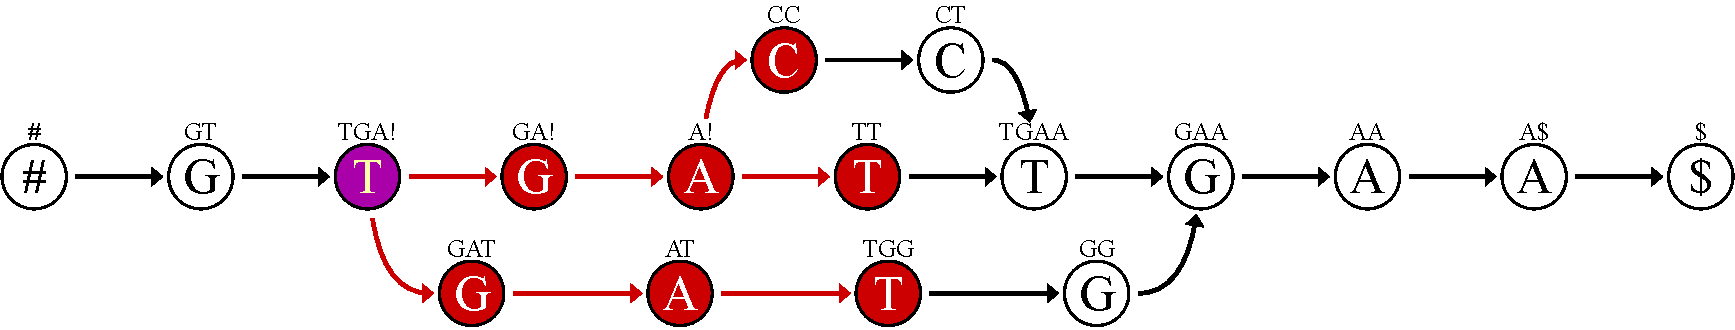
\includegraphics[width=\textwidth]{evo_node_splitting_tree.pdf}
\caption[Graph with prefix generation tree]{Graph with prefix generation tree based on node with prefix \textup{“TGA!”}, having leaves with labels \textup{C, T} and another \textup{T}. These leaves are also highlighted in red here, while the prefix tree visualization in GML usually leaves out the leaves of the prefix generation tree to only highlight the interior nodes which actually agree when building the prefix.} \label{fig:evo_node_splitting_tree}
\end{figure}
Here, we were trying to enlarge the prefix of a node with prefix “TGA!”, 
and got the node with label “A!” as split node. 
It is not necessary to always act as the Graph Merging Library does in this case. 
It would be equally right to first split the node with prefix “TGA!” into two different nodes, 
and to split the node with label “A!” later on.

\subsection{Finding Text Patterns}

Text patters in a graph corresponding to a flat table 
can be found using the \texttt{LF} function with a big initial range which gets diminished through 
several applications, calling the function once for each letter in the text. 
This happens in the \texttt{find} function, the general approach of which is shown in algorithm~\ref{alg:find}. 
\begin{algorithm}
\caption[Find pattern in a flat table]{Find pattern $ P $ in a flat table.}
\addtocontents{loa}{\vskip 15pt}
\label{alg:find}
\begin{algorithmic}[1]

\State $ [ sp, ep ] \gets [ 0, ( \textrm{\textbf{length of} BWT} ) - 1 ] $
\State $ i \gets \textbf{length of} \, P $

\State \phantom{nl}

\While {i > 0}
	\State $ i \gets i - 1 $
	\State $ [ sp, ep ] \gets \texttt{LF} ( [ sp, ep ] , P [ i ] , \texttt{true} , i > 0 ) $
	
	\State \phantom{nl}

	\If { ( \textbf{length of} [ sp, ep ] < 1 ) \textbf{or} ( ep < sp ) }
		\State \Return $ [ \, ] $
	\EndIf
\EndWhile

\State \phantom{nl}

\State \Return $ [ sp, ep ] $

\end{algorithmic}
\end{algorithm}
This function returns a range which corresponds to the nodes 
at which the given pattern $ P $ starts in the graph, 
given using the FC-indexing method. 
This method is used through the last parameter given to \texttt{LF}, which is $ i > 0 $. 
This parameter is do\_rank, and it is \texttt{false} for the last iteration which we 
are looking at, so that \texttt{LF} in the last iteration does not perform the final rank operations 
to convert its output into absolute indices. 
The reason why we wish to use this indexing method here 
is that FC-indexing allows us to specify not just a node, 
but a precise outgoing edge of that node, so that the caller does 
not need to guess which edge to take out of the node. 
However, the caller is still expected to find the rest of the edges manually by 
traversing the graph from the node that was found onwards, 
as they are not directly given out.

\section{Merging Flat Tables}
\label{sec:merging_flat_tables}
%
% ~~~~~~~~~~~~~~~~~~~~~~~~~~~~~~~~~~~~~~~~~~~~~~~~~~~~~~~~~~~~~~~~~~~~~~~~~~~~~~~~~~~~~~~~~~~~~~~~~~~~~~~~~~~~~~~~~~~~~~~~~~~~~~~~~~~~
%                                                                                                         METHODS: Merging Flat Tables
% ~~~~~~~~~~~~~~~~~~~~~~~~~~~~~~~~~~~~~~~~~~~~~~~~~~~~~~~~~~~~~~~~~~~~~~~~~~~~~~~~~~~~~~~~~~~~~~~~~~~~~~~~~~~~~~~~~~~~~~~~~~~~~~~~~~~~

The merging of flat XBW tables is in principle similar to the merging of node tables. 
We again iterate over all nodes of all involved graphs and construct a new table 
based on them. 

A big difference to the merging of the node tables is that we no longer have 
a data structure available to store the computed prefixes of all columns. 
This is intentional, as storing all of these prefixes in memory would be prohibitive 
in a real-world scenario. The implication of not having the prefixes readily available 
are that we can no longer keep track of problematic nodes that easily. 
Therefore, merging the separate tables together as they are and working on the node splitting to expand the prefixes 
after the merge, as we did for merging node tables, is impractical. 
As the flat XBW format relies heavily on the ordering on the columns, 
we simply cannot guarantee that we will order the columns correctly 
if we do not have expanded prefixes in the first place.

We therefore decided to implement the merging of flat XBW tables in three main steps, 
with the first being an iteration over all nodes of the tables that are supposed to be merged, 
with the aim of determining which prefixes will need to be expanded. The corresponding nodes are 
split and the prefixes recalculated already within the input graphs before the actual merge. 
This is repeated until no further node splitting will be necessary when the actual 
merge occurs. \\
The iteration itself occurs as step-by-step comparison in which we advance through 
both input tables at the same time, always choosing to advance with the node that has the lexicographically 
smallest prefix of the considered nodes. 
This is done using the \texttt{checkIfSplitOneMore} function of the XBW environment in GML, 
which calculates one set of prefixes of nodes in both input tables 
and either advances to the next set of nodes, or populates the splitnodes array 
with nodes which it recommends to split to be able to construct unambiguous prefixes if this 
construction is not possible without splitting nodes. 
To return such a split node, \texttt{checkIfSplitOneMore} internally uses the \texttt{\_publishPrefix} function 
described in section~\ref{sec:gml_flat_construct_prefixes}, which can make a recommendation for a 
node that enables us to construct longer prefixes upon being split.
If such a node is returned, then the function \texttt{splitOneMore} is used to actually 
perform the node splitting. \\
Just as when merging XBW node tables as described in section~\ref{sec:gml_merging_node_tables}, 
we again use an aftersort array. 
The reason for using it is that the ordering of the nodes within the first input table is not necessarily the 
same as their ordering within the merged table, necessitating this adjustment to the order of comparison 
for the construction of prefixes and the splitting of nodes.

As the second and main part of the merging algorithm 
we then construct the merged table by again advancing through the 
input tables node for node and always adding the node with the lexicographically smallest prefix 
as next node to the emerging table. The way in which we step through the two input tables 
is exactly the same as in the first step, again using the aftersort array to allow us to 
append nodes to the final table in an ordering different from how they are 
ordered within the input. \\
We use the function \texttt{mergeOneMore} to advance through the nodes of both tables, 
and just like \texttt{checkIfSplitOneMore} it internally uses the \texttt{\_publishPrefix} function 
to calculate one set of prefixes of nodes in both input tables. 
It then appends the node with the lexicographically lowest prefix to the emerging table 
and advances to the next set of nodes. 
It never has to return recommended splitting nodes instead of advancing to the next 
set of nodes, as the actions of the first step ensure that the two input tables 
can be merged in the second step without unambiguous prefixes occurring.

The third and final step in our implementation for merging flat XBW tables 
is to clean up the merged table by removing the end node of the first input graph 
and the start node of the second input graph. 
This is done in the function \texttt{finalizeMerge}. 
These nodes could have also not been added to the merged table in the first place, 
making it unnecessary to perform an extra step in the end. 
This however would have increased the complexity of the second step, which is why we 
decided to perform it as a separate step in the end.

% TODO :: add algorithms! like, all of them!

\section{Fusing Flat Tables}
\label{sec:fusing_flat_tables}
%
% ~~~~~~~~~~~~~~~~~~~~~~~~~~~~~~~~~~~~~~~~~~~~~~~~~~~~~~~~~~~~~~~~~~~~~~~~~~~~~~~~~~~~~~~~~~~~~~~~~~~~~~~~~~~~~~~~~~~~~~~~~~~~~~~~~~~~
%                                                                                                   METHODS: Fusing Instead of Merging
% ~~~~~~~~~~~~~~~~~~~~~~~~~~~~~~~~~~~~~~~~~~~~~~~~~~~~~~~~~~~~~~~~~~~~~~~~~~~~~~~~~~~~~~~~~~~~~~~~~~~~~~~~~~~~~~~~~~~~~~~~~~~~~~~~~~~~

So far, we have investigated how several graphs can be merged together directly, 
how they can be merged when they are encoded as node tables, 
and finally how they can be merged when being encoded as flat tables. 
However, there is another interesting possibility for 
combining two graphs which we would like to look at. 
We decided to refer to this method as \textit{fusing} several tables together, 
as it is inherently different from the actions we perform when merging tables.

\subsection{Fusing Instead of Merging}

As shown in section~\ref{sec:merging_flat_tables}, merging flat XBW tables is rather complex. 
It requires a lot of computations and can lead to a lot of node splitting, 
which might be necessary to ensure unambiguously sortable prefixes along the entire merged graph. 
This leads to an increase in file size as opposed to the total file 
size of the individual graphs that are merged. \\
To explore how these problems might be avoided, 
we decided to implement another way to combining several flat XBW tables. 
In this way, consecutive graphs encoded as flat XBW tables are fused together on their ends, 
meaning that the dollar sign node of one graph is connected with the hash tag node of the next. 
How fusing differs from merging is illustrated in figure~\ref{fig:evo_fig_merge_fuse_diffy}. 
% GTC|,1,C,3 and ACT|,1,,3
\begin{figure}[!htb]
\centering
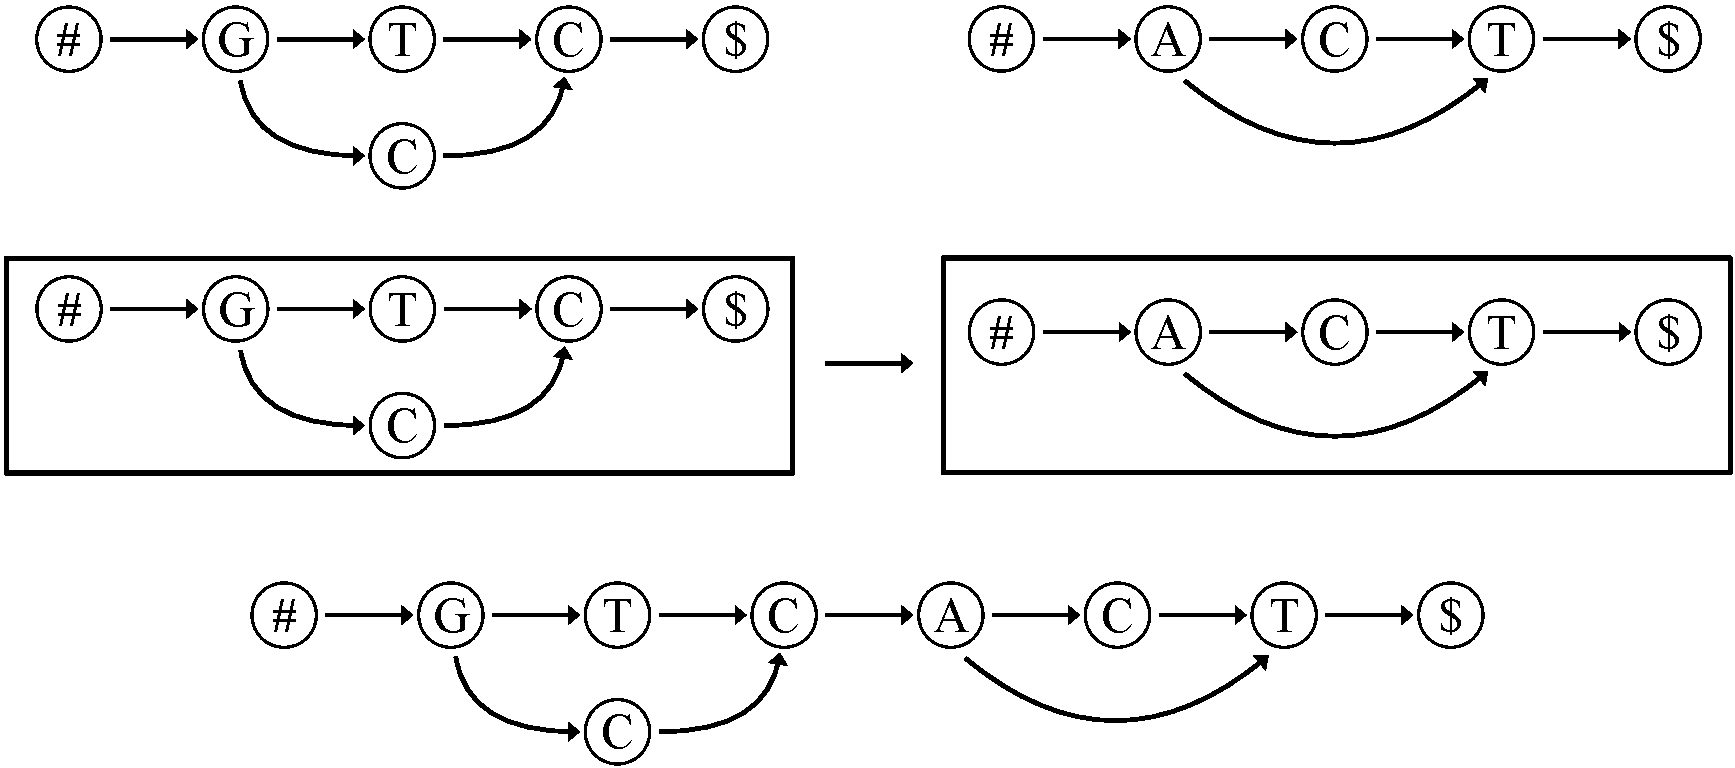
\includegraphics[width=\textwidth]{evo_fig_merge_fuse_diffy.pdf}
\caption[Merging and fusing graphs]{Merging and fusing graphs. The top row contains two input graphs. The middle row shows them fused together. The bottom row shows them merged together.} \label{fig:evo_fig_merge_fuse_diffy}
\end{figure}
This connection is not directly achieved within the flat table itself, 
but it is instead stored in a surrounding host data structure, 
and performed by the program working on it. 
The data structure itself just contains several completely regular flat XBW tables with 
one hash tag and one dollar sign node each, which in addition to the regular information 
can also store information about their immediate predecessors and successors. \\
That is, the core difference between merging and 
fusing is that when we merge two tables, we perform a lot of work once 
to generate one merged table. After the process is finished, 
it is impossible to decide whether the table has been constructed directly 
from some input graph, or has been the result of a merge operation of several graphs. 
On the other hand, when we are fusing two tables together, 
we only perform a relatively small amount work in the moment of fusing them, 
and we then perform a little bit of extra work every time we are operating on the fused table. 
The resulting data structure will always reveal that it actually consists of several 
individual tables, and the extra work needs to be performed every time that the table is operated on. \\
Implementing the fusing behaviour itself is not particularly difficult, 
as the only new occurrence to look out for is a possible spillover in which 
we leave one graph and move on to the next. In that event, the program working 
on the fused XBW data structure needs to automatically jump over the hash tag and dollar sign nodes, 
as internal hash tag and dollar sign nodes should not be accessible to the outside. 
Apart from that, work in a fused table can be performed just like in a regular one.

\subsection{Performing the Fusion of Two Tables}
\label{sec:perform_fusion_of_two_tables}

To actually perform the fusion two flat XBW tables, we create 
a host data structure which has a slot in which it can contain each table. 
We then make each table aware of its immediately succeeding table as well as its immediately preceding table. 
In the case of having two inputs, this means that the first input table needs to store the information 
that there is no preceding table, and that the second input table is its succeeding table. 
Similarly, the second input table needs to store the information that the first table is 
its preceding table, and that it has no succeeding table. \\
In GML, we use the function \texttt{initAsMergeHost} to initialize such a host data structure. 
It contains the array subXBWs, which in turn contains pointers to all tables added to the host data structure. 
The function itself just calls the general initialization function for any XBW environment, 
and then sets an internal integer called role to the value 3. 
Here, the value 1 stands for a regular XBW environment containing exactly one flat XBW table, 
while 2 stands for an XBW environment which is in the process of being merged from several tables 
and 3 stands for an environment which is the host data structure for several flat tables. \\
We then call the function \texttt{addSubXBW}, shown in algorithm~\ref{alg:addSubXBW}, 
\begin{algorithm}
\caption[Add a table to a host data structure]{Add a flat XBW table to a host data structure. The parameter newXBW is a pointer to the XBW environment containing the table which is to be added to the host data structure.}
\addtocontents{loa}{\vskip 15pt}
\label{alg:addSubXBW}
\begin{algorithmic}[1]

\State newXBW.\texttt{\_setPrevXBW}(\texttt{undefined})
\State newXBW.\texttt{\_setNextXBW}(\texttt{undefined})

\State \phantom{nl}

\If {$ \textrm{\textbf{length of} subXBWs} > 0 $}
	\State subXBWs$[ (\textrm{\textbf{length of} subXBWs}) - 1 ]$.\texttt{\_setNextXBW}(newXBW)
	\State newXBW.\texttt{\_setPrevXBW}(subXBWs$[ (\textrm{\textbf{length of} subXBWs}) - 1 ]$)

	\State \phantom{nl}

	\State \phantom{nl}
	\Comment {When fusing, \$ and $\#$ do not need to be replaced}
	\If {we combine tables through merging}
		\State subXBWs$[ (\textrm{\textbf{length of} subXBWs}) - 1 ]$.\texttt{\_replaceSpecialChar}(\texttt{\textquotesingle}\$\texttt{\textquotesingle}, \texttt{\textquotesingle}$\$_0$\texttt{\textquotesingle})
		\State newXBW.\texttt{\_replaceSpecialChar}(\texttt{\textquotesingle}$\#$\texttt{\textquotesingle}, \texttt{\textquotesingle}$\#_0$\texttt{\textquotesingle})
	\EndIf
\EndIf

\State \phantom{nl}

\State reset current positions within the new table to the start

\State \phantom{nl}

\State \textbf{append} newXBW \textbf{to} subXBWs

\end{algorithmic}
\end{algorithm}
once for each table that we want to fuse together within that data structure. 
This function adds the table to the host data structure and connects the table to its predecessor. 
To do so, it first uses the functions \texttt{\_setPrevXBW} and \texttt{\_setNextXBW} to 
set both the preceding table and the succeeding table 
of the new table to \texttt{undefined}, meaning that the new table 
has no preceding or succeeding tables. \\
It then checks if the subXBWs array actually already contains entries, meaning that there 
already are tables stored in the data structure. 
If so, then the succeeding table of the last table in the structure is set to the new table, 
and the preceding table of the new table is set to that last table. 
If we are merging instead of fusing tables together, then the function also 
replaces the end node of the preceding table with “$\$_0$” and the start node 
of the new table with “$\#_0$”. 
This however is not necessary when fusing tables, as the labels of nodes within the 
tables can stay exactly as they usually would, with spillover scenarios being 
completely handled from the outside when algorithms are working on the data structure. \\
Finally, the new table is appended to the subXBWs array, which concludes the fusing of the 
table to the ones already in the data structure before.

\subsection{Fusing More Than Two Tables}

When we want to merge more than two tables, we can simply do so by repeatedly merging pairs 
of two tables together. E.g. if we want to merge the tables representing graphs $ H_1 $, $ H_2 $ and $ H_3 $, 
then we can first merge $ H_1 $ and $ H_2 $ generating table $ H_{12} $, and afterwards 
merge $ H_{12} $ and $ H_3 $ to generate table $ H_{123} $. 
This means that although it might be interesting to look into merging algorithms which can handle 
more than two input tables at once, it is ultimately not entirely necessary to do so, as at least 
theoretically any number of tables can be merged if we are able to merge two tables.

When we intend to fuse several tables together, the situation is slightly different. 
As the process of fusing two tables together does not result in one table, 
but instead in a data structure internally consisting of two tables, 
we need to explicitly enable the fusing process to handle more than two input tables 
and fuse them together into one data structure. 
Furthermore each algorithm working on the fused data structure needs to be able to 
handle such a data structure containing an arbitrary amount of tables, 
as it would not help having a fused table consisting of more than two tables if there 
were no algorithms readily available to perform any work on that fused table. \\
Luckily, the changes needed to be made to the algorithm from section~\ref{sec:perform_fusion_of_two_tables} to 
account for more than two input tables are rather small. 
In particular, the host data structure needs to be able to provide an arbitrary amount of slots into 
which to put these tables, such as an array which can hold as little as one element but has no practical boundary 
in how many elements it can contain. Also, the tables within the structure need to be made aware of the 
correct surrounding tables, each having exactly one preceding table and exactly one succeeding table, 
except for the first table which has no preceding table and the last table which has no succeeding table. \\
We here assume that a data structure representing a fused table always contains at least 
one table, as otherwise it would be pointless to try and perform any work on it anyway. 
The reason why we want to allow one table in the data structure instead of requiring at least two 
of them is that we would like algorithms designed to work on these data structures to also be 
able to handle single flat tables without having to create a whole special case for them in which 
they are used directly without surrounding data structure.

\subsection{Navigating Through Fused Tables}

Just as with the navigation through XBW node tables and regular flat XBW tables, 
we again wish to be able to find the start and end nodes of a fused flat XBW table. 
We also wish to able to find the preceding and succeeding nodes of a 
given node within a fused flat XBW table.

To be able to perform any of these navigation functions, we however first need to 
define an indexing method which can be used within the fused data structure. 
When working with a regular flat XBW table, we can use a single integer $ i $ to 
address a node via the three different methods of FC-indexing, BWT-indexing and absolute indexing. 
As all these methods have certain advantages and disadvantages, we would like to 
keep using them with fused flat tables. \\
In addition to the integer $ i $, which gives us the location within a table, 
we however need to also keep track of which table the node is located in that we are addressing. 
One way is to simply use a second integer $ j $ to encode the table that we are interested in, 
such that each node in the fused graph is identified via a pair $ (i, j) $ of integers addressing the 
node in the table and the table within the structure. \\
However, a second way is to keep using a single integer, and to determine which table we are in 
by adding the lengths of all tables before the addressed one. So if we want to address a node 
with location $ i $ in the second table within a fused structure, we would actually address it as $ | H_1 | + i $, 
where $ | H_1 | $ stands for the amount of nodes in the first table. \\
We decided to use the first of these two methods, as it is not necessary to change all indices 
of succeeding tables if a node in a table gets added or deleted with this method. 
That is, we address each node in a fused table with a pair of integers, the first of which 
can be given via FC-indexing, BWT-indexing or absolute indexing, while the second one 
actually refers to the table we are picking.

Using this pairwise indexing method, we can find the start node of the graph as 
last node of the first table. 
We know that it is a node within the first table due to the fact that we start each path 
through the entire graph 
in the first table, and we know that it needs to be the last node within that table 
as we find the start node within any flat XBW table in the last position due to 
the lexicographical order of its label. 
The index of the start node $ v_s $ of the fused graph 
is therefore $ ( | H_{\textrm{last}} | - 1, 0 ) $, 
where $ H_{\textrm{last}} $ is the last table within the subXBWs array of the host data structure and 
$ | H_{\textrm{last}} | $ is the amount of nodes it contains. \\
It is just as simple to find the end node $ v_e $ of the fused graph. 
It is located in the last table as each path through the entire graph ends there, 
and within that table it is the first node due to the lexicographical properties of 
its label “\$”. 
The index of the end node $ v_e $ of the fused graph 
is therefore $ ( 0, | \textrm{subXBWs} | - 1 ) $, 
where $ | \textrm{subXBWs} | $ is the amount of tables 
that the fused data structure contains.

Just as with regular flat XBW tables, we can also use the $ \Psi $ and \texttt{LF} functions 
to navigate through each table to find preceding and succeeding nodes. 
However, while the behaviour of these functions themselves does not need to change 
at all, we do not call them directly in a fused graph. \\
Instead, we wrap them in special functions provided by the host XBW environment. 
In particular, we can call the function \texttt{host\_$\Psi$} with the same arguments 
as the regular $ \Psi $ function, except for the first parameter 
in which we use a pair $ (i, j) $ to address the node 
we are interested in instead of a plain integer $ i $. 
The result of the function is also slightly different, again being a pair $ (i, j) $ to 
properly address a node within the fused graph instead of a plain integer $ i $. \\
Similarly we have the function \texttt{host\_LF} which now accepts a range of nodes 
within a pair as $ ([sp, ep], j) $ and it gives out an array of such structures. 
It can be seen that this function does not allow us to specify a range spanning more 
than one table, which is intentional. If calculations need to be performed on 
several of the fused tables, such as for pattern searching, then the \texttt{host\_LF} function 
needs to be called on each of the fused tables separately. 
However, several such structure can be returned within an array to be able to return 
ranges in several tables if they are found through spillovers.

% ... - add algorithms for host_Psi and host_LF

\subsection{Prefix Construction}

To construct the prefix a node within the fused table, 
we perform an algorithm similar to the one we performed for the prefix construction 
in regular flat XBW tables. 
In particular, we read out the label of the node itself as starting character of the prefix, 
and then append characters to the emerging prefix by using the \texttt{host\_$\Psi$} function to 
find the succeeding nodes and their labels. 
The only difference to the prefix construction in regular flat XBW tables 
is here that we have to take care of spillovers into succeeding tables, 
which can become especially confusing if we are following several paths which are not all 
within the same table.

% ... write down an algorithm for \texttt{_publishPrefix} in a fused environment,
% or at least make differences to regular algorithm a bit more clear

\subsection{Searching for Patterns}

As with the other algorithms working on fused tables, also the search for a pattern 
in a fused graph is very similar to the algorithm for pattern searches on regular flat XBW tables. 
In particular, we perform a pattern search using the \texttt{host\_LF} function on each table contained 
in the host data structure, while keeping track of spillovers in which a pattern is broken 
across the borders of two tables.

% ... write down an algorithm for \texttt{find} in a fused environment,
% or at least make differences to regular algorithm a bit more clear

\chapter{Results}
% unsere Ergebnisse
%
% ====================================================================================================================================
%                                                                                                                              RESULTS
% ====================================================================================================================================

In this thesis, existing graph reference approaches have been compared 
and new algorithms have been implemented to help the community effort 
of starting to use reference graphs more widely.

\section{Formats for Genomic Graphs}
\label{sec:results_data_formats}
%
% ~~~~~~~~~~~~~~~~~~~~~~~~~~~~~~~~~~~~~~~~~~~~~~~~~~~~~~~~~~~~~~~~~~~~~~~~~~~~~~~~~~~~~~~~~~~~~~~~~~~~~~~~~~~~~~~~~~~~~~~~~~~~~~~~~~~~
%                                                                                                  RESULTS: Formats for Genomic Graphs
% ~~~~~~~~~~~~~~~~~~~~~~~~~~~~~~~~~~~~~~~~~~~~~~~~~~~~~~~~~~~~~~~~~~~~~~~~~~~~~~~~~~~~~~~~~~~~~~~~~~~~~~~~~~~~~~~~~~~~~~~~~~~~~~~~~~~~

We tried out different formats in the course of this thesis, 
and noticed that indeed some do seem more appropriate than others 
for representing genomic graphs 
and in particular population graphs used as alignment references.

\subsection{FASTG Format}

Even though encoding genomic graphs is possible in the FASTG format, 
we noticed that it has some severe drawbacks.

Files in the FASTG format are unnecessarily big, which is mostly caused 
by a lot of intentional whitespaces but also by the decision to repeat the 
default interpretation of each FASTG-specific command just before the command. 
In the following FASTG example, the underlined 
text is just repeated and therefore unnecessary information:

...GCA\underline{TATGTCCTCTCTCC}[1:alt\pipe TATGTCCTCTCTCC\pipe GTC]GG...

On the other hand, when eliminating most of the whitespaces to reduce the file size, 
FASTG files which are already rather difficult to understand quickly 
become more and more obscure, such that they are no longer easily human-readable. 
However, that very human-readability is one of the main advantages of FASTA, 
and without it not much of a reason is left for using this particular family 
of formats altogether.

The FASTG format also is not very flexible. This can be seen by the fact that 
it only allows for three layers of variation within the entirety of the data. \\
The first layer considers global variation that is implemented through a mechanism in which the 
FASTA comments define which sequences can lead to which others. \\
The second layer is about local variation that is implemented through FASTG-specific constructs 
directly in the genomic data. \\
The third layer represents highly localized variation (such as snips) that can be nested 
inside of other FASTG-specific constructs from the second layer. \\
As not all of the constructs can be nested inside of each other 
and as the comment-based global and construct-based local 
variation are completely different approaches, this format 
seems unnecessarily complex.

Finally, the FASTG format as defined in 2012 with 
its many specialized constructs seems to be excessive for 
the needs of the Python test pipeline implemented in the course of this thesis. \\
Trying to implement the entirety of FASTG would in fact 
also be complicated by the fact that the format is open to amendments, 
such that solely implementing the existing standard would not be enough 
to be able to correctly work with all FASTG files which may be encountered. 
Even the specific bubble notation used within many FASTG files 
% which looks similar to ...ACGT[C,T]TAGT... 
does not actually occur in the standard written in 2012 \citep{specGFA1,specFASTG}.

\subsection{GFA Format}

Unfortunately, GFA has several drawbacks as well.

A crucial problem is that GFA has only shortly been worked on, 
and no definitive standard has been published. \\
Although several people have responded quite favourably to the original blog post 
outlining the format, many have also come up with improvements and outright criticism, 
making it less likely that the format in its current state 
is already suited for implementation \citep{knightGFA1}. \\
The lack of a unified standard also means that it is not even clear which version of it 
to base an implementation on.

In the context of this thesis it is also important to consider another drawback. 
According to Heng Li, the author of the format, GFA only aims to be an assembly format \citep{specGFA3}.
% "GFA is not limited to an assembly format. It can represent arbitrary relationship between sequences and is thus suitable for a population graph format in theory. However, I would not take applications on population graphs, such as graph mapping, as a killer application of GFA. There are many open questions on population graphs. I cannot design a format for unsolved questions. GFA aims to be an assembly format only, at least for now."
This means that it can represent a graph based on one particular read assembly. \\
It has not, however, been designed to represent population graphs---which are exactly 
the reference graphs for which it would be helpful to have a useful format.

Finally, this format is very broad and allows for a lot of complicated 
graph behaviour, especially considering its elaborate CIGAR strings. 
This seems to introduce complexity that is, at least for now, 
unnecessary for the purposes of creating a simple 
implementation of a graph reference based alignment tool.

% TODO :: completely overwork this, as apparently the standard came a lot further and now what we wrote here
% a year ago is not correct anymore... oops!

\subsection{Bubble Format}

Surprisingly, implementing an algorithm to open a file in the seemingly simple bubble format was actually 
not easier than implementing more advanced formats like FASTG, GFA and GML.

% TODO :: a bit more text please

\subsection{GML Format}

While using the GML format within the Graph Merging Library, 
it turned out that although it is a simple format for easy graphs, 
modifying graphs with it by hand is rather cumbersome. 
Especially deleting nodes on the main row is a quite elaborate process, 
in which the pointers of all paths leaving or entering the main row 
need to be updated. \\
This problem however could be mitigated by implementing a special text editor 
for the GML format, which would be able to handle common functionalities such as 
removing a node and inserting a node, while automatically updating the relevant pointers.

% TODO :: more

\subsection{FFX Format}

% TODO :: nicer introduction, and maybe also a bit more focus on FFX and what it can / cannot achieve (especially with fused data?)

We noticed that none of the considered formats currently offer inbuilt compression techniques. 
Changing this however would not be very difficult. Especially in the FFX format, 
which mainly contains a BWT and two bit-vectors for each data block, 
a rather simple compression method would be to save both the BWT and the bit-vectors 
using run-length encoding. 
% TODO :: insert figure of FFX with run-length encoding switched on
Such an approach would still keep the format simple enough to be implemented in various 
tools in the future, while offering a significant file size reduction. 
This reduction is especially strong when data is encoded that contains long linear sections 
interspersed with some short graphs, as both of bit-vectors will then 
contain very long runs. \\
It is of course also possible to create even more compressed versions 
of the different formats by not saving the contents of the files as ASCII text, 
but instead as bitwise data structures that can e.g. represent each of the nucleotides A, C, G and T with 
just two bits.

\section{Automated Tests}
%
% ~~~~~~~~~~~~~~~~~~~~~~~~~~~~~~~~~~~~~~~~~~~~~~~~~~~~~~~~~~~~~~~~~~~~~~~~~~~~~~~~~~~~~~~~~~~~~~~~~~~~~~~~~~~~~~~~~~~~~~~~~~~~~~~~~~~~
%                                                                                                             RESULTS: Automated Tests
% ~~~~~~~~~~~~~~~~~~~~~~~~~~~~~~~~~~~~~~~~~~~~~~~~~~~~~~~~~~~~~~~~~~~~~~~~~~~~~~~~~~~~~~~~~~~~~~~~~~~~~~~~~~~~~~~~~~~~~~~~~~~~~~~~~~~~

In general, we can confirm how well the Graph Merging Library functions by checking 
that for a certain set of predefined inputs, the correct outputs are generated. 
For that purpose, we provided several kinds of automated tests for both the 
graph and XBW generation from an input, as well as the merging of several input graphs 
in different ways.

\subsection{Predefined Tests}

The basic approach for testing the validity of the GML algorithms is to run a set 
of predefined tests, for which the correct solutions are known. Doing so will 
show a list of tests and the test results, which can be one of four states. 
Figure~\ref{fig:evo_gml_test_buttons} shows how these predefined tests can be executed in the graphical user interface 
of the Graph Merging Library. \\
\begin{figure}[!htb]
\centering
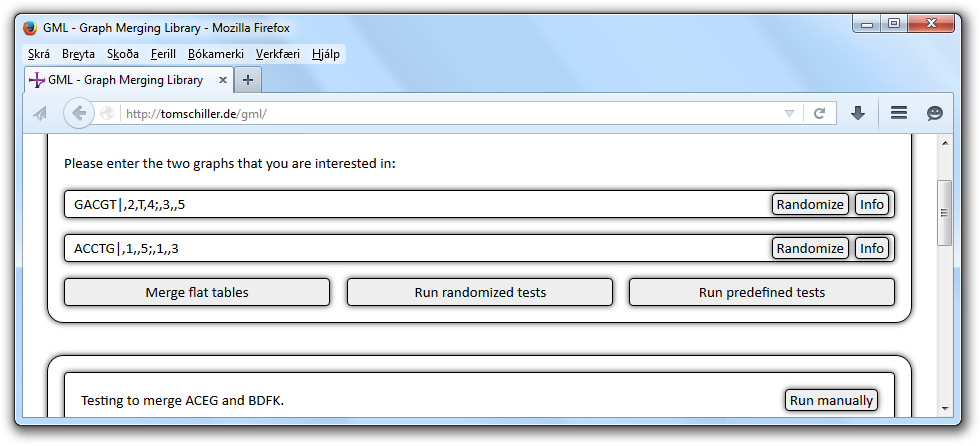
\includegraphics[width=0.95\textwidth]{evo_gml_test_buttons.png}
\caption[GML Test Execution]{GML screenshot with row of three main action buttons. Clicking on the right-most button starts the predefined tests, while clicking on the button on its left starts the randomized tests.} \label{fig:evo_gml_test_buttons}
\end{figure}
The ideal result is a \textit{success}, in which the algorithmically generated result agrees with the 
expected result of the test. \\
Instead, a \textit{failure} can be reported if the result as generated by the GML algorithms 
differs from the expected result. \\
Finally, the label \textit{crash} is associated with a test which causes the 
entire program to crash completely, without generating any useful results whatsoever. 
Ideally, no input data should ever be able to cause this to happen, 
but if it should happen, then a crash would be reported to alarm the user to it. \\
The representations of all these result types in the GML interface can be seen in figure~\ref{fig:evo_gml_different_test_results}. 
\begin{figure}[!htb]
\centering
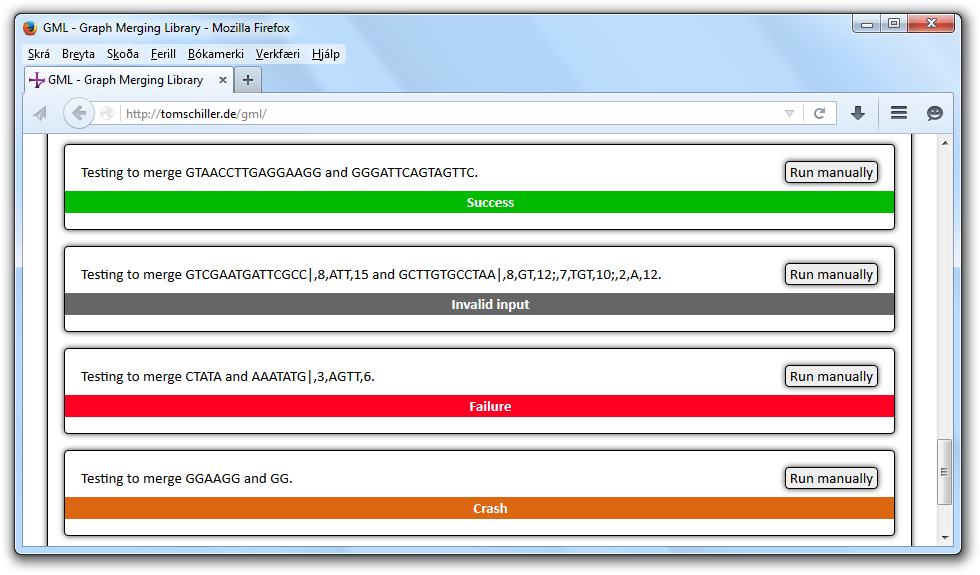
\includegraphics[width=0.95\textwidth]{evo_gml_different_test_results.png}
\caption[GML Test Results]{Different test results in the GUI of the Graph Merging Library.} \label{fig:evo_gml_different_test_results}
\end{figure}
A list of all predefined tests for the construction of XBW node tables can be found 
in section~\ref{sec:appendix_graph_const_tests} in the appendix. 
Section~\ref{sec:appendix_graph_merge_tests} contains the predefined tests for 
the merging of XBW node tables and flat XBW tables. 
Each of these lists also contains a smaller optional section at its end, 
which contains graph inputs which are intentionally invalid. These are used 
to ensure that GML reports an input as invalid when incorrect graphs are entered. 

\subsection{Randomized Tests}

The predefined tests are intended as a method for gouging how well the algorithms 
are functioning, but it could be argued that they might be hand-picked 
to only show positive outcomes. 
Therefore, a second mode of testing has been implemented 
in which random test data is created during the execution time of the program. 
However, generating such random test data automatically means 
that it is difficult to ensure that the input conforms 
to the core assumptions as formulated in section~\ref{sec:gml_core_assumptions}. 
It is in particular difficult to randomly generate test data for which 
no spillover in the splitting of nodes across several graphs which are 
supposed to be merged could possibly happen during the merging process. 
Opposed to that, it is straightforward to ensure that the input graphs 
contain no loops.\footnote{\,\,\,This can be achieved by starting out with a 
random sequence of characters as one path from the start to the end 
of the graph. 
Then new paths can be added one at a time to the emerging 
graph, with each new path from node $ u $ to node $ v $ only being 
allowed to be added if $ v $ could already be reached from $ u $ before 
the new path was added.} \\
It is therefore necessary for the program to ensure that the 
input can actually be worked on, and to give out a warning if not. 
That is why another possible test result with the label \textit{invalid input} can be reported. 
This occurs when the program determines that the input does not conform 
to the previously formulated core assumptions. 

\subsection{Test Analysis}

For the Graph Merging Library to be able to report whether a test is a success or 
a failure, the more robust graph merging from section~\ref{sec:direct_graph_merging} 
is used to generate the result that we 
wish to see. Then, a more advanced algorithm is used for the direct merging 
of XBW node tables or flat XBW tables. 
The resulting flat tables are then compared. 
% GAC|,1,T,3 and AC, on 150%, with tables on 300%
\begin{figure}[!htb]
\centering
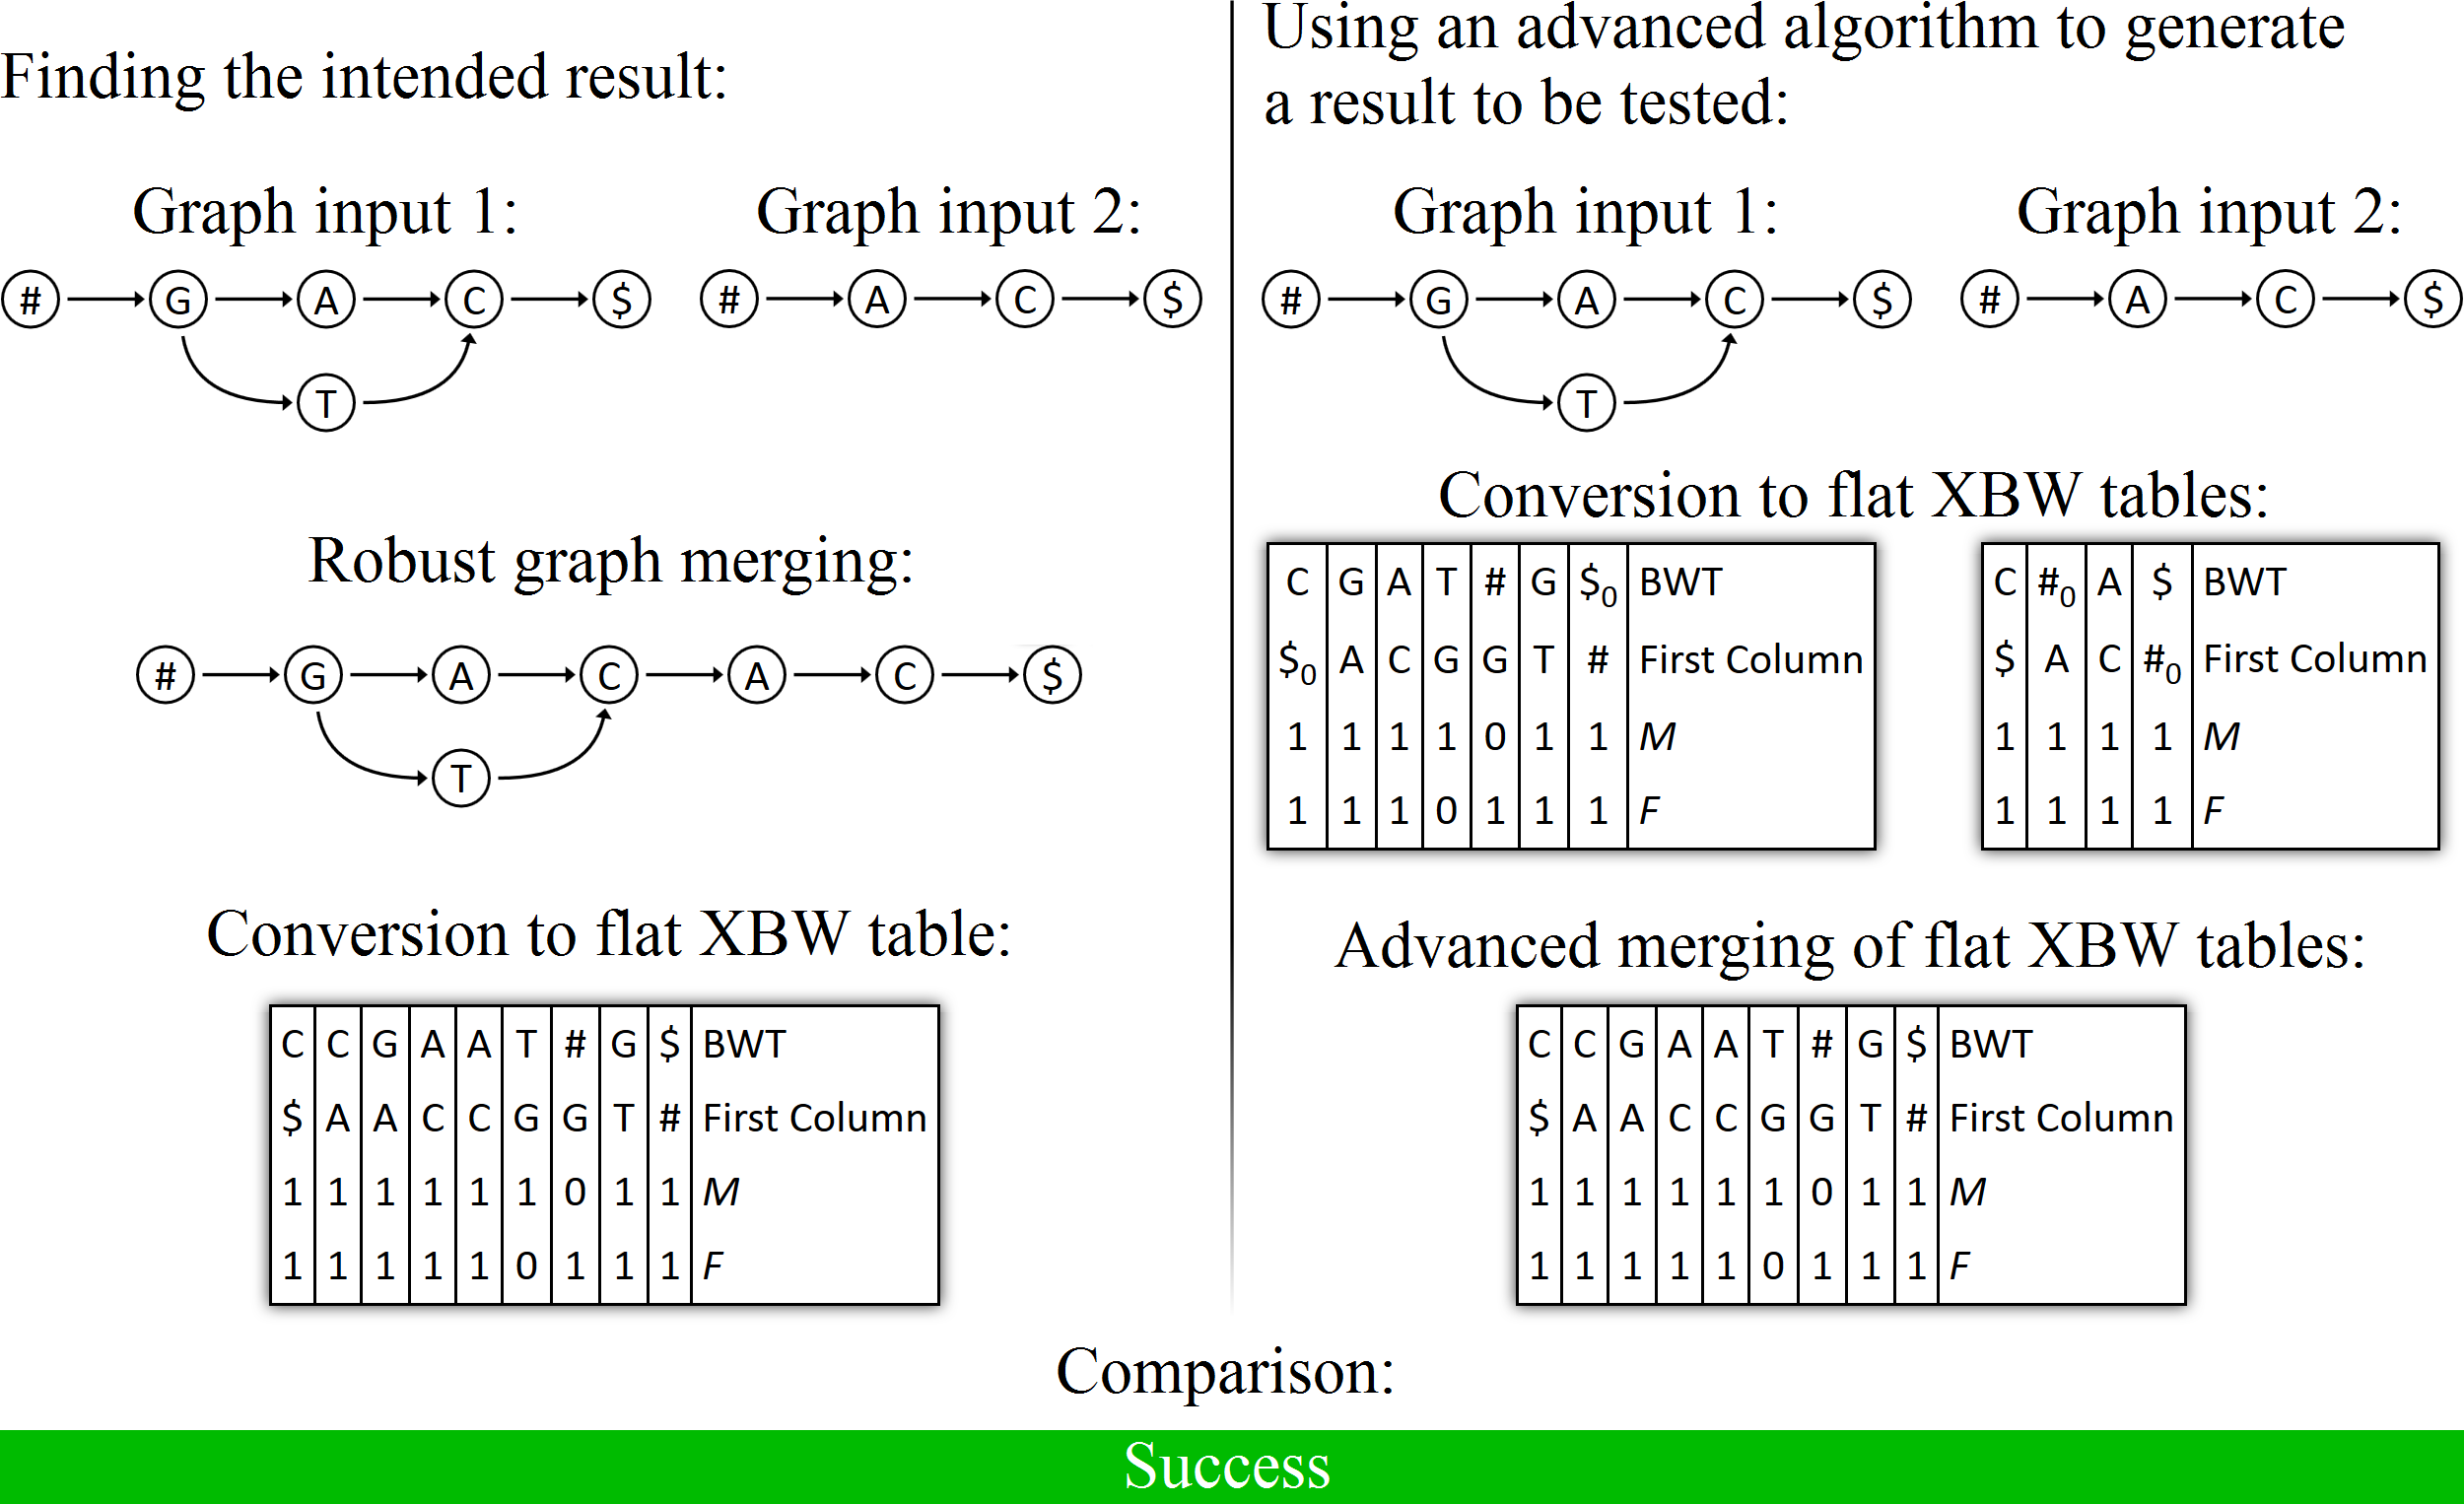
\includegraphics[width=\textwidth]{evo_test_comparison.png}
\caption[Test analysis]{Test analysis by comparison of flat XBW table generated after robust merging of graphs and flat XBW table generated through advanced merging of several flat XBW tables.} \label{fig:evo_test_comparison}
\end{figure}
This approach is illustrated in figure~\ref{fig:evo_test_comparison}. \\
It is however entirely possible for the two tables to be different, but for the result to 
still be a success. That is, the flat XBW table generated through one method and the 
flat XBW table generated through another method can be different if the order in which BWT 
entries within a node are listed is different, as it does not make a difference in which order 
this listing is reported. Also, the tables can be different in case of nodes having been split 
by a method which are not entirely necessary to be split. 
This needs to be considered especially when prefix doubling is used for XBW node table merging, 
as the prefix doubling by design propagates node splits which are not strictly necessary, 
in order to more quickly build prefixes. \\
To be able to compare the results of different methods anyway, and call a test 
a success even if not the exact same flat table has been generated, but a nevertheless 
equally acceptable table has been constructed, we convert the tables in question to the 
primitive automata described in section~\ref{sec:internal_graph_format}. \\
We further introduced the function \texttt{automataAreEquivalent}, which 
takes in two automata to give out \texttt{true} if both are equivalent, 
and \texttt{false} if they are not. We here define two automata to be 
equivalent if they generate the same language, even though they may differ 
in the amount and layout of nodes that they use to construct this language. \\
We can therefore check if both methods that are compared produce flat tables 
which correspond to automata generating the same languages, which means 
that graphs are generated which contain the exact same paths.

Even with the ability to compare the languages generated by automata, 
the automated tests still have to be analysed carefully instead of 
simply being taken at face value. \\
Consider a merge test with several randomized inputs showing a mismatch 
between the expected result and the actual result. 
Usually, this should be reported as a failure because the actual result of the algorithm 
failed to be the expected result. \\
On the other hand, the same behaviour can also occur if the randomized input 
does not conform to the basic assumptions. If the program worked correctly, 
this would be recognized automatically and the input would be flagged as invalid. 
However, if we would report this as a failure then there would be a bug somewhere 
in the program, so that bug could just as well be in the part of the source code 
which detects whether inputs are invalid or not. \\
In general, it is not always entirely clear whether the program failed to provide the correct answer 
because the input was invalid, or because a bug prevented the generation of the correct output. 
The reason for this is that determining whether the input is invalid or not is part of that 
very same source code, and if a bug prevents it from correctly working, then this may be determined 
wrongly. In the opposite way, a bug might also prevent an actually invalid input from being 
flagged that way, resulting in a reported error which actually is no error at all. \\
Overall, this means that both tests which are reported as failures as well as tests which are reported as invalid input 
should be manually investigated more closely to 
better understand the underlying cause of the categorization. 
Having said this, in several thousand testing rounds the categorizations have held up completely, 
and the reported outcome was indeed correct. A more detailed description of the tests which have been performed 
and analysed can be found in the next section.

\subsection{Test Results}

Running the over 100 predefined tests for the XBW creation, node table merging 
and flat table merging in Mozilla Firefox under Microsoft Windows 7 on a 2.40 GHz machine with 4 GB RAM 
resulted in successes for each of them, 
with no failures or crashes being reported. 
As the tests have been picked to include various challenging situations 
in which complicated node splitting behaviours arise and in which 
special sorting mechanisms need to be used to ensure the correct outcomes, 
it can be seen that the algorithms appear to be working fine.

In addition to the predefined tests, we also executed 4,000 tests with randomized data, 
testing the merging results of the flat XBW table merging algorithm. \\
280 of these randomized tests were reported to contain invalid input, 
while the remaining 3720 tests were all reported as successes, 
either generating the exact expected flat XBW tables, or at least 
generating XBW tables which corresponded to graphs which contained exactly the 
correct paths.

% TODO :: add information about node table merging test runs

It should of course be noted here that no amount of tests can ever 
truly prove the Graph Merging Library to truly be working correctly, 
as any amount of tests performed is necessarily finite, while there are 
infinitely many inputs that could theoretically be specified, 
such that it will never be possible to check every single input that there is.

\section{Merging XBW Tables}
%
% ~~~~~~~~~~~~~~~~~~~~~~~~~~~~~~~~~~~~~~~~~~~~~~~~~~~~~~~~~~~~~~~~~~~~~~~~~~~~~~~~~~~~~~~~~~~~~~~~~~~~~~~~~~~~~~~~~~~~~~~~~~~~~~~~~~~~
%                                                                                                                RESULTS: Merging XBWs
% ~~~~~~~~~~~~~~~~~~~~~~~~~~~~~~~~~~~~~~~~~~~~~~~~~~~~~~~~~~~~~~~~~~~~~~~~~~~~~~~~~~~~~~~~~~~~~~~~~~~~~~~~~~~~~~~~~~~~~~~~~~~~~~~~~~~~

Using the Graph Merging Library, we have explored several ways to merge both XBW node tables and flat XBW tables. 
As could be expected, merging two node tables is a much simpler process than merging two flat tables, 
as a node table is less optimized for compression, and working on it is simpler in general. 
The node table not being as compressed as a flat table though means 
that it would not be practical in a real-life scenario to merge these kinds of tables.

However, even when choosing to merge two flat XBW tables, 
the merge result can become unnecessarily large.

% TODO :: insert picture - a graph, another, and then merged soooo big as the thing is split and split and split

\section{Fusing Flat Tables Instead of Merging Them}
%
% ~~~~~~~~~~~~~~~~~~~~~~~~~~~~~~~~~~~~~~~~~~~~~~~~~~~~~~~~~~~~~~~~~~~~~~~~~~~~~~~~~~~~~~~~~~~~~~~~~~~~~~~~~~~~~~~~~~~~~~~~~~~~~~~~~~~~
%                                                                                         RESULTS: Fusing XBWs Instead of Merging Them
% ~~~~~~~~~~~~~~~~~~~~~~~~~~~~~~~~~~~~~~~~~~~~~~~~~~~~~~~~~~~~~~~~~~~~~~~~~~~~~~~~~~~~~~~~~~~~~~~~~~~~~~~~~~~~~~~~~~~~~~~~~~~~~~~~~~~~

When merging flat XBW tables together, it is common that node splitting 
will result in a merged graph with a size larger than the total size of the 
original graphs. 
The method of fusing flat XBW tables together as proposed in section~\ref{sec:fusing_flat_tables} omits 
the need for this increased file size, 
which not only makes it easier to store the data, but also means that working on 
it is quicker as less data means that fewer operations are necessary to construct 
distinct prefixes, to traverse all possible paths, and so one.

However, fusing flat XBW tables also has downsides. 
One of them is related to indexing. 
When working with a merged graph, every column in the graph has a clear integer index, 
so that locations within the entire graph can simply be referred to with a single integer value. 
With a fused XBW however, in addition to specifying a column within the table, 
it also needs to specified which table is addressed, necessitating pairs of integers. 
If particularly large list of locations needs to be created, this difference of two integers instead of one 
could become problematic. \\
Also, it is algorithmically more complex to work with fused graphs, as every 
algorithm working on the graph needs to be prepared to handle spillover scenarios, 
in which the end of one of the fused graphs is reached and the execution needs to continue 
within the next graph. 
Individually, handling each spillover scenario might be only a small amount of effort, 
but when large amounts of work are performed on the table, then these small amounts of work 
could add up to take significantly more time than work performed on a regular table would. \\
These spillover scenarios might also severely limit the otherwise seemingly 
great possibilities for splitting the computation of fused graphs across different 
cores in a distributed system. 
If each processor core is supposed to work on exactly one graph, 
but spillovers are happening frequently, then some cores would stop having work 
to do as no further work would be going on within their data block, 
while others would have to do twice as much work by caring for their 
own work before working on the activity that spilled over from the other data block. \\
Finally, setting up such a system in the first place might be difficult to do, 
as a fused file would most likely contain large areas of linear data, 
fused together with short blocks of graph data. Therefore, assigning one 
data block to one core and letting it perform work in this straightforward fashion 
would lead some cores to have to do much more work than the others, ultimately 
leading to many idle cores waiting for a few to finish which were given much more work 
to do in the first place. This is obviously not desirable in a multi-core system, 
in which ideally all the processor cores should be working for the same time 
and then be done together in the quickest time possible.

However, at least some of these problems could be overcome fairly easily. 
Spillover scenarios as an example, which with a naive 
implementation would possibly lead to some cores having no work to do 
after a spillover happened while other cores would have to do twice as much, 
could be avoided by giving the cores access not only to their own data blocks, 
but also to the data in the surrounding blocks. Then each core could handle 
and complete its own spillovers, without requesting assistance from its neighbours.

\chapter{Conclusions}
% AKA: summarize our data and compare with methodology to see if we fulfilled what we set out to do
%
% ====================================================================================================================================
%                                                                                                                          CONCLUSIONS
% ====================================================================================================================================

Aligning reads from human DNA to graph references rather than to string reference sequences 
still offers many interesting problems. 
However, the first steps on the way to using reference graphs in real-world applications have been made.

\section{Discussion}

Despite a lot of work already having been done to explore 
ways of using genomic graphs within the field of human DNA analysis, 
using reference graphs rather than reference strings still 
is a difficult proposition and only few tools exist that incorporate 
such methods. 
It could therefore be argued that the known advantages of using reference 
graphs do not outweigh the tremendous difficulties that have to 
be overcome in order to be able to use them on a large scale. \\
After all, the reason why reference graphs are proposed to be used 
rather than reference strings is to improve alignment results 
and to simplify the calling of known variants. 
But at least in the beginning when only small local graphs are incorporated 
into largely linear references, the improvements are likely to be very slim. 
Likewise, it could be questioned whether simplifying the calling of variants really 
justifies complicating matters so much in general by the introduction of 
these new graph structures.

However, we would argue that in the long run, reference graphs will come to be used. 
With every new individual DNA that is constructed, more insight is gained into 
variations which could be quite common among populations. 
Discarding all of that data in favour of a simpler but ultimately flawed approach 
will not work forever, as over time better alignment results will come to be expected. \\
Therefore, it seems inevitable to work on reference graphs eventually, 
and it seems only logical to start that work as soon as possible, rather than investing 
more time and resources into improving current alignment tools which are likely to be drastically 
modified to incorporate reference graphs in the future anyway.

\section{Future Work}
% AKA: Possibilities for SOMEONE ELSE to make it even better

There still remains a lot of future work to be undertaken to actually use 
the already existing and the here newly proposed algorithms in real-world 
tools of the analysis pipeline. 
As various different tools are in use for specific problems, no one implementation 
is likely to achieve this. Instead, the community at large needs to start 
incorporating the ideas of using graph data rather than sequential data into 
more and more of the existing tools.

\bibliography{thesisreferences}

\appendix
\renewcommand{\chaptername}{Appendix}
\chapter{Appendix}
%
% ====================================================================================================================================
%                                                                                                                             APPENDIX
% ====================================================================================================================================

\section{Predefined Graph Construction Tests}
\label{sec:appendix_graph_const_tests}
%
% ~~~~~~~~~~~~~~~~~~~~~~~~~~~~~~~~~~~~~~~~~~~~~~~~~~~~~~~~~~~~~~~~~~~~~~~~~~~~~~~~~~~~~~~~~~~~~~~~~~~~~~~~~~~~~~~~~~~~~~~~~~~~~~~~~~~~
%                                                                                        APPENDIX: Predefined Graph Construction Tests
% ~~~~~~~~~~~~~~~~~~~~~~~~~~~~~~~~~~~~~~~~~~~~~~~~~~~~~~~~~~~~~~~~~~~~~~~~~~~~~~~~~~~~~~~~~~~~~~~~~~~~~~~~~~~~~~~~~~~~~~~~~~~~~~~~~~~~

% TODO :: keep these lists up to date!

The following tests are run to ensure that the Graph Merging Library does not throw errors 
while constructing flat XBW tables for input graphs:

\begin{lstlisting}
ACEG
ACEG|,1,,3;,2,TB,4
GACGTACCTG|,2,T,4;,3,,5;,6,,10;,6,,8
GACGTACCTG|,2,,4
ACGTAGATTTC|,4,,7
TAATACGCGGGTC|,8,,9
GACGTACTG|,5,C,8;,2,G,5;,5,GT,9
GCTGGCGAGCAG|,3,T,6;,5,TC,12;,5,,7
GCTGGCGAGCAG|,3,T,5;,5,GCTC,12
GACGTACCTG|a,2,TAT,6;,a:0,C,a:2
GACCTAATG|,5,C,8;,2,G,5
ATTCACCACCAACCCGACATA|,4,CACG,9;,9,TCG,12
CCACGCGCCATGGC|,1,CTG,14
GCTGGCGAGCAG|,3,T,5;,5,,7
GCTGGCGAATGTGGCAAGAATGTGGCAAGAGCAG|,3,T,5;,5,,7;,4,CACG,9;,9,TCG,12
GCCGT|,3,,5
ATCT|,2,A,3
ATCGAT|,2,,5;,4,CG,6
TGATGAG|,6,,7
GTTAATGTGGCAAGT
TCCCTGT
CTACCAGGTGCTGTTATTCCAC|,16,A,22
CTATGTTATTCCA|,8,A,13
TATA|,2,A,4
CCA|,1,A,2
TTCGCAAGA
CCTGCGTGTGGT|,3,,6
CCGAGCTTATCGCAA
ATGCGAGTTCGGGAC|,9,CCCG,14
GCAGGGAGCTCCAGCCGTTAG|,4,CC,13;,1,A,18;,17,,19
ATTGGAGAAGTCACGCTTGAC|,6,CTA,14
CACTC
TGCAAGTATGGCGCTT|,2,,8
AACCAT|,4,GGG,6
AACCAT|,4,GGG,6
AGAGCACGCCGGT
AGAGCACGCCGGT
CGGCAATAGACGCTGTCCAATGC|,15,,18
AGAGCAT
ACTGGCATGATTTATCCCTTGG|,11,,12
GGGCCCAGGGCGATCGACGTTC|,7,,19
CCCAGCC|,4,,6
CAGCC|,2,,4
CACT
CACT
TC|,1,C,2
ATCAACTTTCC|,6,CA,7
GCGGTGAAGAGAAA|,2,CGG,7
CCACGCTAAGTTATCGTGT
ATCCAATCGTAAT|,7,T,8
TAGCTTGGAC|,2,AG,9
GACAAACACAAACATCACCCTGT
CGTCGCC|,6,T,7
AAAGTAT
TACTTGTC
GCAGAATTCCGCAGGAAAGC
CGCGACAGTGGCCAATCT
GGTACATGGGAT
TCTGGTACGCTG|,1,,11
GGGAACAGATGTCTGTGATCC|,13,CAT,14
CGAGTTACGTGGCCGCCTCAT
TGTCTGTTACAGATTGC
CGAAGCCTA
CGAAAGAGTGTGTCTAGGC|,11,TC,19
TTTAGGTTAGTACCAC|,8,CTG,11
TACTTCCCCAGGACGGGACGCTA
AAAGGAGGT|,7,,8;,2,A,6
GGTGGCCGAGTGC|,10,CTGC,12
CGAATACCGTACTGAA|,12,AAAA,15;,14,GGTC,15
TTCCAATGGTGAGTCTC
AAGAT|,2,CTC,3;,1,C,4
AACAAATT|,4,TCCT,8
AAAAGAAGCTGAT|,4,,6
ACGTGCCCACCCG|,2,A,8
TAGGCGCGGT
TTTGCATCATATC
TTGTAG|,5,A,6
CTATATAGCGGC|,4,CTA,7
ATTAATACG|,2,G,5
CGGCCT|,1,A,6;,2,TT,4
CATCTTTC|,5,CA,7
AGGCAGCTATCGACCATCTTGCG|,22,,23;,2,TT,9;,9,C,10;,22,,23
AAGAGTCCAGAG|,7,,11;,5,TATA,9
GCCACGACACCCTCAAGCT|,17,CA,18
TTAAA|,4,GAT,5
TACCAGGGCTTTTTTACTGGCT|,8,,19;,20,GCT,21
TGAAGCGCATTCT|,9,,11;,3,,11
CGGATAGCACTCTA|,9,TT,11
TCCCTGGGC
CAAGGTATTGTTAA
CTCGGCTCT|,1,AAGG,2;,4,,6;,8,TG,9
AGGGAGCCTTAACATTTTCG|,13,T,19;,11,AGCG,15;,10,A,12
TCAGGGCGAGC|,6,G,9
GGAGCCAGGCTTGCCC|,7,,11
TGGCCCTCCCCCTACAT
AGGCCATTGATGAAAA|,7,AT,9;,5,CCT,12
GTATGCT|,6,TACC,7
ATTATCGATCA|,3,TCT,7;,10,CGCT,11;,8,TTCA,11
GTAACCTTGAGGAAGG
GTCGAATGATTCGCC|,8,ATT,15
CTATA
GGAAGG
\end{lstlisting}

The following tests are run to ensure that GML correctly recognizes whether a dataset is an invalid input:

\begin{lstlisting}
GACGTACCTG|,2,T,12;,3,,5;,6,,10;,6,,8
GACGTACCTG|,4,T,2;,3,,5;,6,,10;,6,,8
GACGTACCTG|,2,T,4;,a:3,,5;,6,,10;,6,,8
ATCTCAG|,1,GG,4;a,2,C,6;,a:1,G,7
\end{lstlisting}

\section{Predefined Graph Merge Tests}
\label{sec:appendix_graph_merge_tests}
%
% ~~~~~~~~~~~~~~~~~~~~~~~~~~~~~~~~~~~~~~~~~~~~~~~~~~~~~~~~~~~~~~~~~~~~~~~~~~~~~~~~~~~~~~~~~~~~~~~~~~~~~~~~~~~~~~~~~~~~~~~~~~~~~~~~~~~~
%                                                                                               APPENDIX: Predefined Graph Merge Tests
% ~~~~~~~~~~~~~~~~~~~~~~~~~~~~~~~~~~~~~~~~~~~~~~~~~~~~~~~~~~~~~~~~~~~~~~~~~~~~~~~~~~~~~~~~~~~~~~~~~~~~~~~~~~~~~~~~~~~~~~~~~~~~~~~~~~~~

% TODO :: keep these lists up to date!

The following tests are run to ensure that the Graph Merging Library does not throw errors 
while merging XBW tables for input graphs:

\begin{lstlisting}
ACEG and BDFK
ACEG|,1,,3 and BDFK
ACEG|,1,,3;,2,TB,4 and BDFK|,2,,4
C and ACTG|,2,,4
C and ACATG
GACGT|,2,T,4;,3,,5 and ACCTG|,1,,5;,1,,3
C and ACTG|,2,T,4
GACGT|,2,C,4;,2,T,4;,3,,5 and ACCTG|,1,,5;,1,,3
GACGT|,2,T,4;,1,C,4;,3,,5 and ACCTG|,1,,5;,1,,3
TAT and C
TT|,1,A,2 and C
TCGTGCGAGG|,1,ACAA,10 and C
TAATACGCGGGTC|,8,,9 and ACCTG|,1,,5;,1,,3
AAGTTTCTTTCGTGCGAGGCCGT|,10,ACAA,19;,16,CGT,20 and ACCTG
ATAGTCAATTGACTGCCGACG and CGGGGTAAAAAAGCGCC
GCCG and GCGC
GCCG and BDFK
GG and CGG
ATCT|,2,A,3 and CC
ATCGAT|,2,,5;,4,CG,6 and C
TGATGAG|,6,,7 and GCCAGGTCAGCCTAGTCCCTG
GTTAATGTGGCAAGT and CTCGCGACGACTAAAGCTGGCC
TCCCTGT and CTCAGCAGAGGCCCAGGCAAA|,13,TA,15
CTACCAGGTGCTGTTATTCCAC|,16,A,22 and CATCGATTT|,3,CGAT,9
CTATGTTATTCCA|,8,A,13 and C
TATA|,2,A,4 and C
CCA|,1,A,2 and CA
TTCGCAAGA and TCCCCAAG
CCTGCGTGTGGT|,3,,6 and CTCTTA|,3,TCG,5
CCGAGCTTATCGCAA and GAGAGAGCAAC
ATGCGAGTTCGGGAC|,9,CCCG,14 and TCCAA
GCAGGGAGCTCCAGCCGTTAG|,4,CC,13;,1,A,18;,17,,19 and CGGAT
ATTGGAGAAGTCACGCTTGAC|,6,CTA,14 and GTTAAAACAC|,6,TC,10
CACTC and GGGCAGTACGTGG|,9,,11;,7,CGCG,8
TGCAAGTATGGCGCTT|,2,,8 and GTGTAATTATGAAC|,13,GATG,14
AACCAT|,4,GGG,6 and GTGCAGCTTTTGG
AACCAT|,4,GGG,6 and TTAAGGTTATGGACCCCCC|,4,GGAT,8;,6,C,12
AGAGCACGCCGGT and TTAAGGTTATGGACCCCCC|,4,GGAT,8;,6,C,12
AGAGCACGCCGGT and CGTAAATAGAG|,7,G,9
CGGCAATAGACGCTGTCCAATGC|,15,,18 and CGTAAATAGAG|,7,G,9
AGAGCAT and AGTGAACACAC
ACTGGCATGATTTATCCCTTGG|,11,,12 and TTTGTTTGACACGCTGC|,16,,17;,11,AGGG,14
GGGCCCAGGGCGATCGACGTTC|,7,,19 and TTTGTTTGACACGCTGC|,16,,17;,11,AGGG,14
CACT and GCGTACG|,5,,7;,1,C,5
CACT and GCGTACG|,4,,7;,1,C,5
TC|,1,C,2 and TC
ATCAACTTTCC|,6,CA,7 and TACCGAACGCCGGTGTGATAA|,6,,8
GCGGTGAAGAGAAA|,2,CGG,7 and GACTC
CCACGCTAAGTTATCGTGT and GCTTTATACGTAAT|,10,CC,13
ATCCAATCGTAAT|,7,T,8 and TCGAATTATCACGATAT|,13,AAA,17;,12,CG,15;,7,,15;,7,GAG,16
TAGCTTGGAC|,2,AG,9 and GTGATGT|,5,,7
GACAAACACAAACATCACCCTGT and TGAAATAGT|,4,T,6
CGTCGCC|,6,T,7 and TCAATGTATAGTCGTGTCTGAAAT|,8,TGCA,23
AAAGTAT and AAAGCGAGCAAAAGATTGACGAA
TACTTGTC and CTCAACT|,6,,7
GCAGAATTCCGCAGGAAAGC and CATGGCGTCTAGGA|,10,GC,12
CGCGACAGTGGCCAATCT and TCGTCTGATGATCTTTGCTCTC|,19,,20
GGTACATGGGAT and ATGCGCTCGAAGCACGAAGG|,6,AT,15
TCTGGTACGCTG|,1,,11 and ATGCAAAAGTTTAAAGTTGTCCGT|,3,CGCT,18
GGGAACAGATGTCTGTGATCC|,13,CAT,14 and TGAAAAAAACTCAGCGGGGAGT
CGAGTTACGTGGCCGCCTCAT and CCGTA|,3,TGT,5
TGTCTGTTACAGATTGC and AGACATCCATC|,4,,11;,10,TC,11
CGAAGCCTA and TTGTGAATATCG|,6,CTG,9
CGAAAGAGTGTGTCTAGGC|,11,TC,19 and AGAGCT
TTTAGGTTAGTACCAC|,8,CTG,11 and CATAGCTTAGCC|,11,,12
TACTTCCCCAGGACGGGACGCTA and GGTCAG
AAAGGAGGT|,7,,8;,2,A,6 and GAGTTATGACG
GGTGGCCGAGTGC|,10,CTGC,12 and CATTTGTGGCGCGCTTGATCTCTG|,10,,20
CGAATACCGTACTGAA|,12,AAAA,15;,14,GGTC,15 and ACAGCGAGAGCAGACG|,14,TC,15;,8,,16
TTCCAATGGTGAGTCTC and ATAAAG|,3,AG,5
AAGAT|,2,CTC,3;,1,C,4 and ACGCTCCTTTGTGG
AACAAATT|,4,TCCT,8 and GAGCGGAGAATCATACGGGC|,16,GAG,20;,1,CGC,17
AAAAGAAGCTGAT|,4,,6 and CTTGAA
ACGTGCCCACCCG|,2,A,8 and CCCCAACTGGGAATTC|,13,TCC,16;,4,TTT,14
TAGGCGCGGT and CTGGGACGG|,4,GTG,7;,2,C,6;,4,TGA,7;,6,C,9
TTTGCATCATATC and GAAACATTTATGACATTA|,4,,12
TTGTAG|,5,A,6 and AACGCGT|,3,,6
CTATATAGCGGC|,4,CTA,7 and ACGCATATTGGTTC
ATTAATACG|,2,G,5 and TTTTTATGGTCCGACTAA
CGGCCT|,1,A,6;,2,TT,4 and TTAATCT
CATCTTTC|,5,CA,7 and GTTGGTGGCCATCGG|,11,,15;,4,GG,14
AGGCAGCTATCGACCATCTTGCG|,22,,23;,2,TT,9;,9,C,10;,22,,23 and AGCTGGGAAAC
AAGAGTCCAGAG|,7,,11;,5,TATA,9 and AGTGGCTGATTGGT
GCCACGACACCCTCAAGCT|,17,CA,18 and TCAATTGCCGGTA
TTAAA|,4,GAT,5 and GAACTCGGGGC|,3,TTGT,5
TACCAGGGCTTTTTTACTGGCT|,8,,19;,20,GCT,21 and CCGGCGGATTGATAGTGC
TGAAGCGCATTCT|,9,,11;,3,,11 and GGATGCGAGCAGTACGTCTCCTTC
CGGATAGCACTCTA|,9,TT,11 and ATGTTGGGCCCTAA|,7,A,12;,8,T,11
TCCCTGGGC and ACGATTCCCTAACCACCCGT|,17,ATG,19;,7,TT,16
CAAGGTATTGTTAA and AGTCTAAGGCTTCGTGTTGGATC|,9,GTA,22
CTCGGCTCT|,1,AAGG,2;,4,,6;,8,TG,9 and AAAGTCTTCAATGT
AGGGAGCCTTAACATTTTCG|,13,T,19;,11,AGCG,15;,10,A,12 and CATGTTGGTTGT
TCAGGGCGAGC|,6,G,9 and GACAACCCAGATTTTCCCGCATT|,10,,18;,15,TAA,17
GGAGCCAGGCTTGCCC|,7,,11 and ACAGGATAGGTCATTGAGTGGGG|,11,CAAC,16
TGGCCCTCCCCCTACAT and TAGGCCGAAGTTTCTCTATCTTG|,13,CAAA,18;,16,AAC,19
AGGCCATTGATGAAAA|,7,AT,9;,5,CCT,12 and GACTG|,2,,3
GTATGCT|,6,TACC,7 and GGACCTACGGCGGTTTAAAA|,8,A,14;,2,GCGA,12
ATTATCGATCA|,3,TCT,7;,10,CGCT,11;,8,TTCA,11 and TGACAAGGTGCTCAGGTGAAA
GTAACCTTGAGGAAGG and GGGATTCAGTAGTTC
GGAAGG and GG
AATTCGGTAATACCGAAG|,15,AT,17 and TAAGATAAGGCAAA|,7,TA,11
CAGAGTATGCTCCGAG and CGATTACGCAT|,8,,10;,3,TA,9
GACGCCGACAAGAGACAAG|,2,CCA,11;,17,TC,18 and AGGTAGT
GTATAAATACAAGCTAAG|,17,CCA,18 and GATGA|,3,TCTC,4
CTAGA|,2,CC,3 and AAGATGAAAGGACCCCCA|,16,,18
GGGGAAAGCAAGATATCAGCCGT and CAAAAAGA|,4,,5;,3,C,5
ATGATG|,4,TC,6 and AAATGAGAT|,7,TGC,9;,5,AG,8
GCCAGA|,3,TAC,5 and CAACTCCAGGTTCCCTTATTG|,11,GTCA,13
GATATGGCGT|,3,A,9;,7,GTCA,10 and AAGACTTATACGC|,11,,13;,3,G,10
GCGGATATTTGGCGGCT|,6,A,14;,12,GTCA,15 and AAGGAAGAAGACTTATACGCC|,18,,20;,10,G,17
TGGAAGCACACCC and TAGGGCGGAAGGG|,5,A,11;,5,TCCT,11;,8,GCCC,12
GTGCCCTAGACCTCCTTAT|,5,,10;,13,CCA,14;,7,GT,11;,3,G,8;,12,TGGG,18 and GTGCA
TGTACTGGCTCCTATAT and TAACACATTAGTCAACCACA|,13,,16;,5,,12
CGACAG|,5,TTCC,6;,3,T,5 and GACCCACGCAAGAAACCGTGA|,10,TAAC,19
CGTTTGCATGAATTTGTTT and AACGTACCATTAAAATAGCGA|,6,,9;,4,TG,20
TACGATCGGA|,2,ATCG,6 and TAAGTTA|,2,CTG,3
GAGTATAAGCCA|,9,,10 and GGCGCGGTCAGTT|,12,GC,13;,2,GAT,6
AACCA|,4,CTTT,5;,4,CA,5;,4,ACG,5 and AGGTTATAGAT|,7,CAT,9;,2,,11
TCCGCTT|,2,TTTG,6;,4,ACT,6;,3,GGTG,6;,5,AACG,7;,2,ATC,5;,4,,5;,3,AA,6;,3,GGA,7 and TCGACATTGCTGCAGGTT|,14,CT,18
CCCAGCC|,4,,6 and TT|,1,AGG,2
CAGCC|,2,,4 and TT|,1,AGG,2
TTCCGCGGCTCCATG|,14,CGTA,15 and ACCGTCCTCA|,8,CCGT,9;,8,C,10;,4,,10
ACTCTGAATGCTGTACACTCA|,5,,19;,13,C,14;,17,AGA,21 and GTTTGGGGA|,6,,9
ACCTG|,3,AAC,5;,1,C,2;,1,C,2 and ACGATGAAACGGATTGTA
TACACG|,4,AAT,6;,1,CCGA,5 and TGGTGTATTATTGCCCTTGGACGC|,20,GA,22;,5,G,17;,8,AATA,10
TGTAGATGAGCATACCCCGA|,4,ACGA,20;,11,,19;,15,TT,19;,6,,11;,13,AA,20 and AAATATCTTTGTTG
CTCATACGAGCGAA|,12,CG,13 and GTGCCCGGGTGCA|,1,TTTC,11
TTTTAATAGTCACCGATCCGG|,17,CGTT,21;,19,TTT,20 and TCGGCATT|,4,ACGA,7;,6,GGA,8;,3,TGA,8
CCCAATGACAATG|,7,TAGA,10;,5,ACCC,10;,4,C,11;,4,,8;,8,C,11;,7,AGGT,9 and GTGTC
GCTAGTTACAACT and GCAAGCGAA|,3,TCG,4;,5,T,8
CAGTTTACAACTGCAGCCGTTA|,7,,12 and TCGCCCGTAACTCAACGTTTAA|,16,CTGG,17;,19,A,20;,19,GC,20
AACCCT|,1,ATCA,3;,2,C,4;,3,,5;,4,TCAT,6 and CCTTCGTACTAGCACAAACT|,5,GGTT,11
TTGCTAACCAGC|,4,TC,5 and GGTGTTTGGGGCCCATACAAAT|,15,A,18;,1,GA,11;,5,CCGC,14;,10,,19;,5,,13
\end{lstlisting}

The following tests are run to ensure that GML correctly recognizes whether a dataset 
consisting of two graphs which are supposed to be merged contains an invalid input:

\begin{lstlisting}
CTATA and AAATATG|,3,AGTT,6
GTCGAATGATTCGCC|,8,ATT,15 and GCTTGTGCCTAA|,8,GT,12;,7,TGT,10;,2,A,12
TGGCC|,1,TA,2 and ACGCAGCTGCGAGAATA|,1,ACCC,5
GTAGCAAAGCGGTTTGGGATTG and GGTACCTATAGGGAA|,2,C,5
GAGTGGCCAAGTAGCCGGGTCACA|,23,GTC,24 and CGTACTG|,3,GAGC,7
GGTGGGATGGACTCTGTTGTG|,12,CACA,18 and CTGACTGTCAGGAGCTGA|,3,,9
GGTACGCGTTATCGT and CTGTCTATCTCTAACCC|,12,,16;,2,T,6;,11,GA,12
GTAAC and TTTCACGCGT|,5,C,10;,5,CTC,6;,1,CG,3;,8,A,9
GTAATGACGTAGCCC and ATCATCGCA|,3,CT,8
GGGTTAGCTGTCTAAG|,6,C,9 and ATGATGATA|,5,ATAT,6;,1,TA,2
GTAGAGAATGGACTACTG and TGTGTGTTC|,2,ACG,4
ACGCAAGATGTATC|,3,GGAC,9;,10,G,11 and CCCCT|,2,CTT,5
TCGTCGTGAG|,5,G,6 and GAACCCGGAATCTTA|,2,T,15
ACTCGTGAAG and GGGCA|,1,CTCA,5
ATACGTAATCGGTGGCTCGA|,14,TCG,20 and AGATCGAGCTG|,4,,10;,8,,10;,2,CTA,7
ATGTACACTTCTGAGTTGTCC and GCGTTGCG|,1,G,4
CGGAGACTATCCTATCC|,9,CAG,15;,11,,16 and CAGTCATCGATTAAACCACTCTG|,1,GG,5
TGCTGCTTTGGAAAT|,1,ATTA,14 and GTCCGTAGCAA|,5,GG,7;,1,,7
GCTCTCATGCAGCCCAA and TTTCAGCCTAACAGTACACGGGT|,1,GA,19
CGCCC|,4,GAC,5;,4,,5;,3,ATG,4 and CAAGCTG|,1,GTTA,5;,5,GA,6
ACTCCTACTCCAACTA|,9,GTT,13 and ACTACC|,4,ATG,6
AACTAGGCGCATGTC|,3,CAG,8;,3,GTT,15 and CTTGGC|,3,AGA,6;,2,T,4;,2,CTAT,4;,1,AT,2
\end{lstlisting}

\section{Resources and Licensing}
%
% ~~~~~~~~~~~~~~~~~~~~~~~~~~~~~~~~~~~~~~~~~~~~~~~~~~~~~~~~~~~~~~~~~~~~~~~~~~~~~~~~~~~~~~~~~~~~~~~~~~~~~~~~~~~~~~~~~~~~~~~~~~~~~~~~~~~~
%                                                                                                    APPENDIX: Resources and Licensing
% ~~~~~~~~~~~~~~~~~~~~~~~~~~~~~~~~~~~~~~~~~~~~~~~~~~~~~~~~~~~~~~~~~~~~~~~~~~~~~~~~~~~~~~~~~~~~~~~~~~~~~~~~~~~~~~~~~~~~~~~~~~~~~~~~~~~~

Publicly available genomic datasets as well as automatically generated data were used 
to implement the new graph reference approaches and to analyse the results of the implementations.

Recently, there has been a push towards implementing more open source scripts 
and programs within the scope of bioinformatics \citep{MANIFESTO}. \\
All of the software developed while working on this thesis 
is open source and distributed under the terms of 
the Creative Commons Attribution Non-Commercial License 
(\url{http://creativecommons.org/licenses/by-nc/3.0/}), 
% TODO :: check (ask someone?) if this is the correct license to be used here
which permits non-commercial re-use, distribution, and reproduction in any medium, 
provided the original work is properly cited. 
For commercial re-use, please contact \url{moyaccercchi@hotmail.de}. \\
The source codes together with the newest version of this thesis itself can be accessed at \url{http://tomschiller.de/graphalign}.
% 
% TODO :: add stuff to the appendix!

%
%
% don't let any reference remain unused!
% \phantom{
% References that are so far not referred to anywhere else in the text:
% }
%
%

\end{document}

% TODO :: check if all our lists are in the following format
%
% ullet list
% Hér á eftir er dæmi um upptalningarlista. Listinn má vera þéttari, 
% þ.e. að aðeins sé 0 pt bil á milli atriða, en þó skal hafa 12 pt bil á undan fyrsta atriði listans.
% \begin{itemize}
%  \item Númer 1
%  \item Númer 2
%  \item Númer 3
% \end{itemize}
% Ef fyrsta lína eftir upptalningu er framhald sömu málsgreinar og fyrir ofan 
% skal ekki setja inn viðbótarloftun (eða ef inndráttur er notaður, 
% skal ekki nota inndrátt á slíkri línu).

% TODO :: check if all our figures and tables are in the following format
% 
% \chapter{Figures and tables}
% { \color{red} Þessi kafli sýnir dæmi um notkun mynda, taflna og vísun í þær. }
% 
% \section{Figures}
% { \color{red} Myndatexti skal staðsetja undir myndum og skrifast með skáletri.
% Setja skal auða aukalínu fyrir ofan myndir.
% \begin{figure}[!htb]
% \centering
% 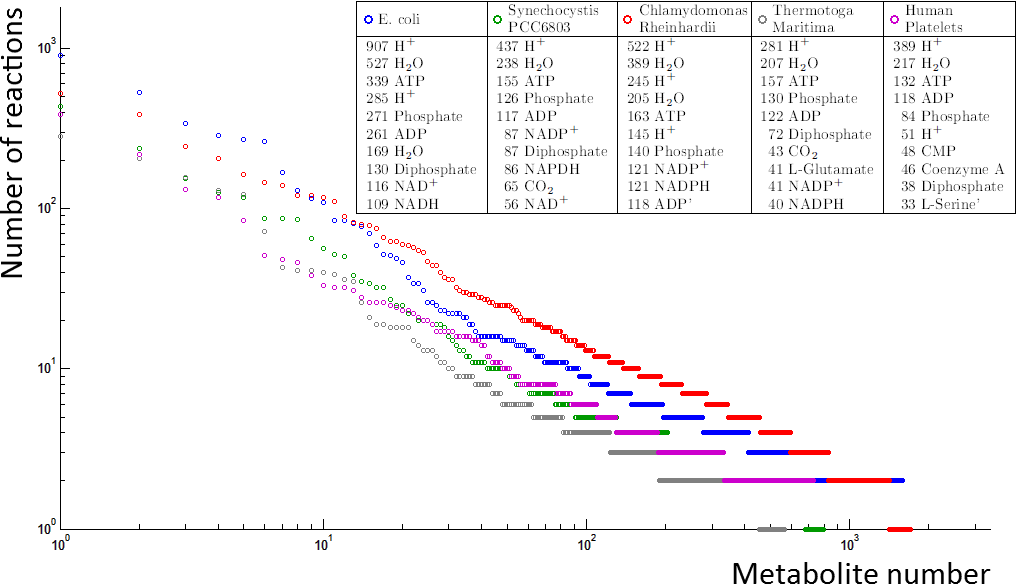
\includegraphics[width=0.47\textwidth]{evo_example_pic.png}
% \caption[Dæmi um myndatexta (fyrir neðan mynd).]{Dæmi um myndatexta (fyrir neðan mynd)} \label{fig:Example Pic}
% \end{figure}
% Mikilvægt er að skilgreina myndir með ,,paragraph format”: “keep with next” til að rjúfa 
% ekki tengsl á milli myndar og myndtexta. Mynd má vera miðjuð og skal þá einnig miðja myndartextann. 
% Letur innan myndar skal vera í steinskrift (sans serif), t.d. Verdana, og ekki minna en 10 pt. 
% Tryggið að letur, tákn og línur sjáist skýrt eftir útprentun.
% 
% Hægt er að láta númera og merkja myndir sjálfvirkt með því 
% að gera Insert – Reference – Caption – Mynd eða Tafla. 
% Varist að velja hyperlink. 
% 
% Vísa má í mynd með því að velja Insert – Reference – Cross-Reference – Mynd eða Tafla. 
% Varist að velja hyperlink og veljið að eins Label og Number. 
% T.d. sjá þessa tilvísun í Mynd 3.1 sem dæmi. }
% 
% \section{Tables}
% { \color{red} Einnig má númera töflur sjálfkrafa svipað og myndir. 
% Nota skal skáletur í töflutitil. Textinn skal standa fyrir ofan töflu og fylgja töflunni. 
% Ekki nota tvöfalt línubil eða hafa space before í töflum. 
% Meginreglan við töflugerð er að hafa þær einfaldar og eins fá strik og mögulegt er. 
% Tafla má vera miðjuð á blaðsíðu og skal þá láta töflutitil byrja við vinstri brún töflu.
% 
% \begin{table}[htb]
% \centering
% \caption{Dæmi um töflutexta (fyrir ofan töflu).}
%      \sffamily \begin{tabularx}{1.0\textwidth}{ p{5cm}  p{5cm}  p{5cm} }
%     \hline
%    \textbf{Taflan} \hfill & \textbf{Er} \hfill & \textbf{Eins} \\ \hline
%     Og & Hún & gæti\\
%     Litið & Út & í ritgerð\\ \hline
%     \end{tabularx} \normalfont
% \label{table:Emissivity}
% \end{table}
% 
% Almennt skal ekki nota loftun fyrir neðan texta í töflu, og stylla loftun fyrir neðan á 0 pt.
% Mikilvægt er að skilgreina töflutexta með ,,format paragraph: keep with next og keep lines together” til að 
% rjúfa ekki tengsl á milli töflutexta og töflu. 
% Ef tafla er mjög löng má kljúfa hana á milli blaðsíðna og þá verður 
% að setja (\textit{Framhald}) í aukalínu beint fyrir neðan töfluna, 
% hægri stillt við hægri brún töflu.
% 
% Dæmi um sjálfvirka tilvísun í töflu, bara nota Label and Number, 
% ekki nota hyperlink eða caption text. T.d. Tafla 3.1 sýnir dæmi um töflu. }
